\documentclass[notitlepage]{report}
\usepackage{amssymb}
\usepackage{indentfirst}
\usepackage{polski}
\usepackage[english,polish]{babel}
\usepackage[utf8]{inputenc}
\usepackage{xcolor}
\usepackage{mathtools}
\usepackage{blkarray}
\usepackage{amsmath}
\usepackage{float}
\usepackage{graphicx}
\usepackage{siunitx}
\usepackage[nottoc,numbib]{tocbibind}
\usepackage[justification=centering]{caption}
\usepackage[
backend=biber,
style=numeric,
sorting=ynt
]{biblatex}
\usepackage[bookmarksopen=false]{hyperref}
\usepackage{listings}
\usepackage{color}
\usepackage{makecell}
\usepackage{multirow}
\definecolor{dkgreen}{rgb}{0,0.6,0}
\definecolor{gray}{rgb}{0.5,0.5,0.5}
\definecolor{mauve}{rgb}{0.58,0,0.82}
\lstset{frame=tb,
	language=Python,
	aboveskip=3mm,
	belowskip=3mm,
	showstringspaces=false,
	columns=flexible,
	basicstyle={\small\ttfamily},
	numbers=none,
	numberstyle=\tiny\color{gray},
	keywordstyle=\color{blue},
	commentstyle=\color{dkgreen},
	stringstyle=\color{mauve},
	breaklines=true,
	breakatwhitespace=true,
	tabsize=3,
	literate={ą}{{\k{a}}}1
	{Ą}{{\k{A}}}1
	{ę}{{\k{e}}}1
	{Ę}{{\k{E}}}1
	{ó}{{\'o}}1
	{Ó}{{\'O}}1
	{ś}{{\'s}}1
	{Ś}{{\'S}}1
	{ł}{{\l{}}}1
	{Ł}{{\L{}}}1
	{ż}{{\.z}}1
	{Ż}{{\.Z}}1
	{ź}{{\'z}}1
	{Ź}{{\'Z}}1
	{ć}{{\'c}}1
	{Ć}{{\'C}}1
	{ń}{{\'n}}1
	{Ń}{{\'N}}1
}

\hypersetup{pdfstartview={XYZ null null 1.00}}
\hypersetup{pdfpagemode=UseNone}
\addbibresource{bibliography.bib}

\frenchspacing

\begin{document}
	
\setcounter{page}{3}
\begin{abstract}

Celem niniejszej pracy było porównanie wybranych metod ekstrakcji cech z sygnału elektroencefalograficznego w kontekście skuteczności klasyfikacji
stanu aktywności mózgu. Badania przeprowadzono w grupie 17 osób, które wykonały trzy zadania związane z różnymi stanami mentalnymi: relaksacją, pobudzeniem oraz rozwiązywaniem problemu logicznego. Sygnały elektroencefalograficzne zebrano za pomocą kasku Emotiv EPOC+. Na sygnałach została wykonana ślepa separacja źródeł za pomocą analizy składowych niezależnych. Do parametryzacji sygnałów wykorzystano metodę Welcha, modelowanie autoregresyjne oraz dyskretną transformację falkową. Wymiarowość wektorów cech została zredukowana za pomocą analizy składowych głównych. Do klasyfikacji wykorzystano klasyfikator $k$-najbliższych sąsiadów, maszynę wektorów nośnych oraz sieć neuronową.
\\ \\
\textbf{Słowa kluczowe}: elektroencefalografia, interfejs mózg-komputer, ekstrakcja cech, analiza sygnału, klasyfikacja
\\ \\
\textbf{Dziedzina nauki i techniki, zgodnie z wymogami OECD}: Nauki inżynieryjne i techniczne, inżynieria medyczna
\end{abstract}
\selectlanguage{english}
\newpage
\begin{abstract}
The aim of the study was a comparison of electroencephalographic signal
feature extraction methods in the context of effectiveness of the 
classification of brain activities. For the purpose of classification electroencephalographic signals were obtained using Emotiv EPOC+ device from 17 subjects in three mental states (relaxation, excitation, solving logical task). Blind source separation by means of Independent Component Analysis was performed on obtained signal. Welch method, autoregressive modelling and Discrete Wavelet Transform were used for feature extraction. Principal Component Analysis was performed in order to reduce dimensionality of feature vectors. Support Vector Machine, $k$-Nearest Neighbours and Neural Network were employed for classification.
\\ \\
\textbf{Keywords:} electroencephalography, brain-computer interface, feature extraction, signal analysis, classification
\\ \\
\textbf{OECD field of science and technology}: Engineering and technology, medical engineering 
\end{abstract}
\selectlanguage{polish}

\tableofcontents

\chapter*{Wykaz ważniejszych skrótów i oznaczeń}
\addcontentsline{toc}{chapter}{Wykaz ważniejszych skrótów i oznaczeń}
\noindent \textbf{BCI} - interfejs mózg-komputer, ang. \textit{Brain Computer Interface} \\
\textbf{DWT} - dyskretna transformacja falkowa, ang. \textit{Discrete Wavelet Transform} \\
\textbf{EEG} - elektroencefalografia \\
\textbf{ICA} - analiza składowych niezależnych, ang. \textit{Independent Component Analysis} \\
\textbf{k-NN} - $k$-najbliższych sąsiadów, ang. \textit{$k$-nearest neighbours} \\
\textbf{MLP} - perceptron wielowarstwowy, ang. \textit{Multilayer Perceptron} \\
\textbf{PCA} - analiza składowych głównych, ang. \textit{Principal Component Analysis} \\
\textbf{PSD} - widmowa gęstość mocy, ang. \textit{Power Spectral Density} \\
\textbf{RBF} - radialna funkcja bazowa, ang. \textit{Radial Basis Function} \\
\textbf{ReLU} - ang. \textit{Rectified Linear Unit} \\
\textbf{SVM} - maszyna wektorów nośnych, ang. \textit{Support Vector Machine} \\



\chapter*{Wstęp}
\addcontentsline{toc}{chapter}{Wstęp} \markboth{Wstęp}{}

Interfejs mózg-komputer (ang. \textit{Brain-computer interface}, BCI) jest to system umożliwiający bezpośrednią wymianę informacji pomiędzy mózgiem użytkownika a komputerem bez użycia medium pośredniego, jak dźwięk czy obraz, ani bez dodatkowych urządzeń typu klawiatura. Badania nad interfejsami mózg-komputer motywowane są między innymi wspomaganiem interakcji z otoczeniem osób niepełnosprawnych \cite{machado} \cite{nicolasalonso}. 

Obecnie próby realizacji takich systemów są najczęściej przeprowadzane w oparciu o badanie elektroencefalograficzne (EEG). Badanie to polega na pomiarze potencjałów elektrycznych na powierzchni czaszki pacjenta. Głównymi zaletami elektroencefalografii są nieinwazyjność oraz względnie niski koszt. Pobrane w ten sposób sygnały charakteryzują się jednak znacznie gorszym stosunkiem sygnału do szumu niż w przypadku, gdy potencjały elektryczne są mierzone bezpośrednio na powierzchni mózgu. Trudniej jest też określić obszar mózgu, który spowodował aktywność elektryczną w danym punkcie czaszki \cite{shenoy} \cite{hill}.

W systemach BCI zarejestrowany sygnał poddawany jest wstępnej obróbce, mającej na celu, między innymi, eliminację przewidywanych zakłóceń - szumu sieci energetycznej, zakłóceń wynikających z aktywności mięśniowej (niekiedy trudnej do powstrzymania, jak np. mruganie powiek), a także dryftu sygnału. Opcjonalnie sygnał może być też poddany zabiegowi ślepej separacji źródeł. Służą do tego takie metody, jak np. analiza składowych niezależnych (ang. \textit{Independent Component Analysis}, \textit{ICA}). Następnie sygnał poddawany jest ekstrakcji cech, czyli redukcji sygnału do wektora parametrów o niższej wymiarowości. Redukcja taka ma na celu umożliwienie odróżnienia sygnałów reprezentujących różne rodzaje aktywności umysłowej które system BCI ma rozpoznawać \cite{nicolasalonso} \cite{lotte2}.

Celem pracy jest porównanie przydatności wybranych metod analizy sygnałów oraz metod klasyfikacji w zadaniu rozpoznawania stanów mentalnych na bazie zarejestrowanego sygnału EEG. W ramach laboratoriów z przedmiotu \textit{Diagnostyka i protetyka słuchu i wzroku} użyto kasku Emotiv EPOC+ do pobrania sygnałów elektroencefalograficznych od 17 osób, znajdujących się w trzech różnych stanach mentalnych. Pobrane sygnały zostały poddane ślepej separacji źródeł za pomocą ICA. Do ekstrakcji cech z sygnałów wybrano metodę Welcha (służącą do estymacji widmowej gęstości mocy sygnału), modelowanie autoregresyjne oraz dyskretną transformatę falkową. Otrzymane wektory cech zostały zredukowane za pomocą analizy składowych głównych (ang. \textit{Principal Component Analysis}, \textit{PCA}). Do klasyfikacji sygnałów użyto trzech metod klasyfikacji: $k$-najbliższych sąsiadów, sieci neuronowej oraz maszyny wektorów nośnych. 

Organizacja niniejszej pracy jest następująca: rozdział pierwszy przybliża historię badania elektroencefalograficznego i opisuje jego przebieg, a także faktyczne i potencjalne zastosowania. Zawarty jest również opis kasku Emotiv EPOC+ użytego do pobrania sygnałów EEG. Rozdział drugi zawiera opis wstępnego przetwarzania, któremu poddane zostały pobrane sygnały.
Rozdział trzeci zawiera opisy metod analizy sygnałów, które zostały użyte do ekstracji cech. Rozdział czwarty opisuje zasadę działania zastosowanych metod klasyfikacji. W rozdziale piątym opisano zastosowaną technikę redukcji wymiarowości wektorów cech. W rozdziale szóstym opisano przeprowadzone eksperymenty oraz omówiono uzyskane wyniki. W pracy zawarto również wnioski i bibliografię związaną z tematem pracy dyplomowej.

\chapter{Elektroencefalografia}
\section{Historia encefalografii i jej zastosowania}
Aktywność elektryczna mózgu została odkryta w 1875 roku przez angielskiego lekarza Richarda Catona. Podłączył on powierzchnię mózgu żywego królika do galwanometru, za pomocą którego zarejestrował impulsy elektryczne \cite{haas}. W 1924 roku niemiecki psychiatra Hans Berger jako pierszy zarejestrował aktywność elektryczną mózgu u ludzi. Badanie wykonane przez Bergera, w przeciwieństwie do badania wykonywanego przez Catona, nie było inwazyjne. Berger mierzył potencjały elektryczne na powierzchni czaszki, a nie mózgu. Jest on tym samym uznawany za konstruktora pierwszego na świecie elektroencefalografu. Berger opublikował wyniki swoich badań pięć lat później w swojej pracy \cite{berger}.

Niedługo po publikacji wyników badań przez Bergera badanie EEG zaczęto wykorzystywać do diagnozy padaczki. Nawet obecnie ten obszar pozostaje jednym z głównych zastosowań tego badania \cite{smith}. Inne medyczne zastosowania badania EEG obejmuje diagnoza uszkodzeń mózgu \cite{ianof}, określanie głębokości narkozy \cite{simon}, diagnostyka śpiączki \cite{sutter} czy też stwierdzanie śmierci mózgu \cite{webster} \cite{lee}. Badanie EEG można też wykorzystać do diagnozy guzów mózgu oraz wylewu, ale straciło ono na znaczeniu wraz z pojawieniem się rezonansu magnetycznego i tomografii komputerowej.

Termin interfejs mózg-komputer został zaproponowany przez prof. Vidala z Uniwersytetu w Los Angeles w pracy \cite{vidal}. Niedługo później amerykańska agencja rządową Defense Advanced Research Projects Agency (DARPA) wdrożyła badania nad możliwością wykorzystania fal mózgowych do komunikacji \cite{miranda}. Przez całe lata 70. i większość lat 80. zainteresowanie tą dziedziną było ograniczone, a postępy znikome. Jedną z przełomowych prac z dziedziny BCI  opublikowali w 1988 roku Farwell i Donchin \cite{farwell}, w której opisali opracowany przez nich system wypisujący na ekranie komputera litery alfabetu pod wpływem sygnału nazwanego później sygnałem P300. W tym samym roku Bozinovski, Sestakov i Bozinovska opublikowali pracę \cite{bozinovski}, w której opisali system BCI służący do sterowania robotem mobilnym. Od tego czasu zainteresowanie tematyką interfejsów BCI znacząco wzrosło \cite{lebedev} \cite{kubler} \cite{lotte3}.
\section{System 10-20}
Najpowszechniej obecnie stosowanym wzorcem umieszczenia elektrod na czaszcze pacjenta jest wzorzec zwany systemem 10-20. Układ ten został zaproponowany przez Jaspera w 1958 roku w pracy \cite{jasper}. Rozmieszczenie elektrod w systemie 10-20 przedstawiono na rysunku 1.1.

\begin{figure}[H]
	\centering
	\makebox[\textwidth][c]{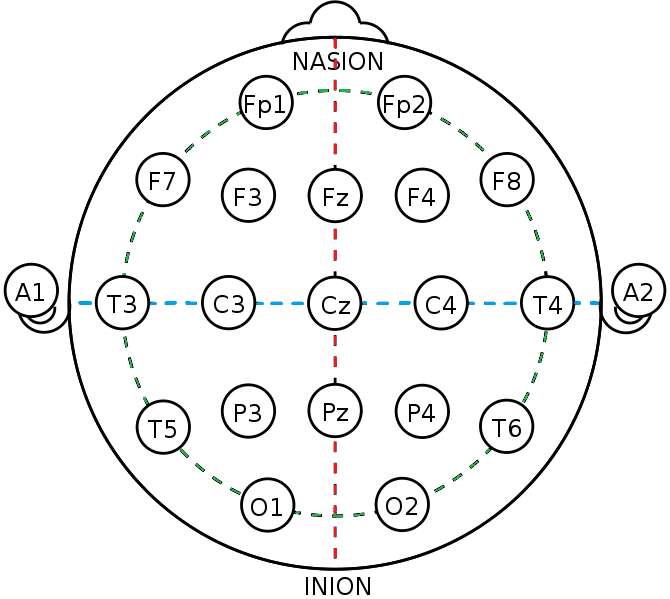
\includegraphics[width=0.8\textwidth]{system1020.png}}%
	\caption{Umieszczenie i nazwy elektrod w systemie 10-20 \cite{1020system}}
\end{figure}
Liczby 10 oraz 20 oznaczają procenty długości krzywej przebiegającej pomiędzy dwoma punktami czaszki, w literaturze anglojęzycznej określanymi jako \textit{nasion} oraz \textit{inion} \cite{jasper}. \textit{Nasion} jest punktem łączenia kości nosowej z kością czołową. \textit{Inion} z kolei jest najbardziej wypukłym punktem łuski potylicznej, będącej częścia kości potylicznej. 
Punkty te, wraz z wyznaczoną przez nie krzywą podzieloną na odcinki, przedstawiono na rysunku 1.2.

Elektrody oznaczone literą F umieszczone są na części czaszki pokrywającej płat czołowy (łac. \textit{lobus frontalis}) mózgu. Literą P oznaczono elektrody pokrywające płat ciemienionwy (łac. \textit{lobus parietalis}) mózgu. Litery T oraz O oznaczają elektrody pokrywające odpowiednio płat skroniowy (łac. \textit{lobus temporalis}) oraz płat potyliczny (łac. \textit{lobus occipitalis}). Liczbami nieparzystymi oznaczone są elektrody umieszczone po lewej stronie czaszki, zaś parzystymi - po prawej \cite{jasper} \cite{teplan}. Elektrody umieszczone wzdłuż linii \textit{nasion}-\textit{inion} nie mają indeksu numerycznego - zamiast tego oznaczone są literą \textit{z}. Elektrody A1 i A2 przymocowywane są do płatków uszu.


\begin{figure}[H]
	\centering
	\makebox[\textwidth][c]{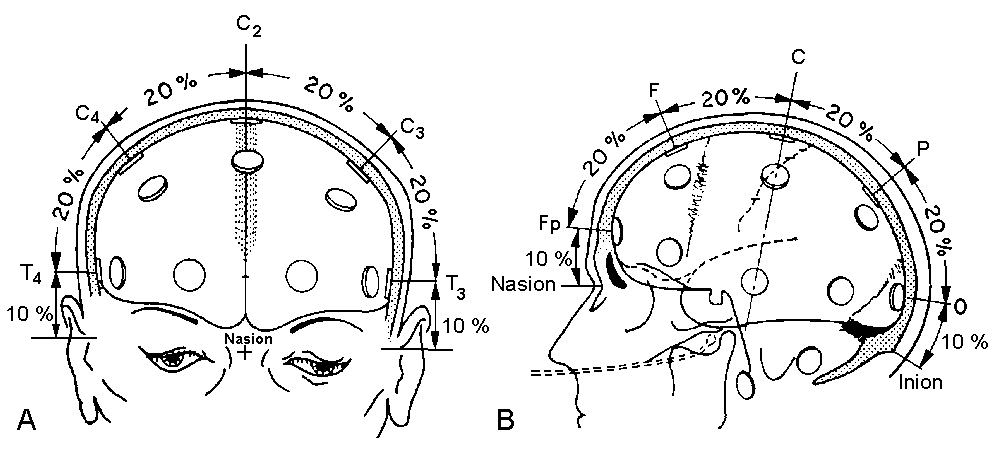
\includegraphics[width=1.2\textwidth]{system1020-2.png}}%
	\caption{Punkty \textit{nasion}, \textit{inion} oraz wyznaczona przez nie krzywa podzielona na odcinki stanowiące 10\% i 20\% całkowitej jej długości \cite{jasper}}
\end{figure}

Istnieją też inne standardy, przewidujące zastosowanie większej liczby elektrod. Rozszerzony system 10-20, zwany także systemem 10\%, opisany został w pracy \cite{nuwer}. Rozkład elektrod w systemie 10\% zaprezentowany został na rysunku 1.3. W systemie 10\% rząd elektrod AF leży w połowie odległości pomiędzy rzędami Fp i F, rząd FC w połowie odległości pomiędzy rzędami F i C, rząd CP pomiędzy rzędami C i P, oraz rząd PO pomiędzy rzędami P i O. Kolumna 1 leży w połowie odległości pomiędzy kolumnami Z i 3. Kolumna 5 leży w połowie odległości między 3 i 7. Analogiczne rozszerzenie następuje po prawej stronie czaszki. W systemie 10\% elektrody T3, T4, T5 oraz T6 niekiedy występują ze zmienionymi nazwami, odpowiednio T7, T8, P7 oraz P8 \cite{nuwer}.

\begin{figure}[H]
	\centering
	\makebox[\textwidth][c]{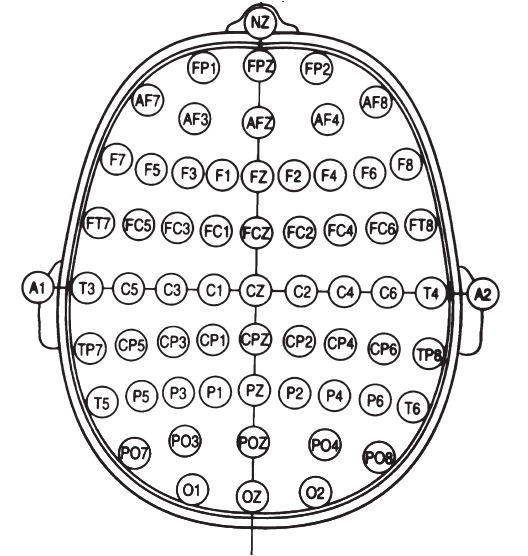
\includegraphics[width=0.8\textwidth]{system10.png}}%
	\caption{Rozkład elektrod w systemie 10\% \cite{nuwer}}
\end{figure}


\section{Przebieg badania elektroencefalograficznego}
Niedostateczna długość lub jakość snu, niski poziom cukru we krwi, używanie alkoholu, kofeiny, nikotyny czy też innych środków psychoaktywnych, leków wpływających na percepcję oraz czuwanie wpływa na wynik badania EEG. W związku z tym pacjent poddawany badaniu powinien być wyspany, nie powinien odczuwać głodu oraz powinien unikać środków psychoaktywnych na 24 godziny przed badaniem - chyba że badanie ma na celu zbadanie wpływu jednego z tych czynników na elektroencefalogram pacjenta. Przed badaniem pacjent powinien umyć głowę, nie powinien natomiast stosować środków do stylizacji włosów. 

Badanie EEG wykonuje się w pozycji siedzącej lub leżącej. Na głowę pacjenta zakładany jest czepek z przymocowanymi elektrodami. Elektrody powinny być przymocowane do wybranych miejsc na głowie, wyszczególnionych w wybranym systemie (np. w systemie 10\%). Elektrody przedtem powinny być nasmarowane żelem/pastą przewodzącym/ą lub nasączone roztworem soli. Medyczne elektroencefalografy najczęściej posiadają przynajmniej 16 elektrod, choć może być ich znacznie więcej \cite{teplan} \cite{lantz}. 

Medyczne badanie EEG powinno trwać przynajmniej 20 minut. W trakcie części badania pacjent powinien mieć zamknięte oczy, a w pozostałej części otwarte. W czasie badania można stosować rozmaite techniki stymulacji, jak np. sygnały świetlne, dźwiękowe czy też hiperwentylacja \cite{sinha}. 

Aktywność mięśniowa silnie zaburza elektroencefalogram, dlatego pacjent powinien w miare możliwości powstrzymać się od mrugania oczami i ruszania kończynami, chyba że badanie ma na celu zbadanie wpływu tych anomalii na wynik badania.

\section{Pasma aktywności mózgu}
Sygnał elektroencefalograficzny często poddawany jest analizie częstotliwościowej. Na jej podstawie można wyróżnić pięć podstawowych pasm częstotliwości, w których występuje aktywność mózgu. Aktywność w poszczególnych pasmach utożsamiana jest ze stanami świadomości badanego, jak np. sen, relaksacja, pobudzenie czy aktywność intelektualna. Należy zaznaczyć, że poszczególne rodzaje aktywności nie występują w całym mózgu, a tylko w jego wybranych partiach. Na rysunku 1.4 przedstawiono przykładowe wykresy pięciu rodzajów aktywności mózgu.

Fale delta są falami o częstotliwośći poniżej 4 Hz i względnie dużej amplitudzie. Utożsamiane są głównie z wolnofalową fazą snu u dorosłych osób, występują wtedy we wzgórzu lub w korze mózgowej. Ponadto, występują one również podczas czuwania - u noworodków jest to dominująca forma aktywności mózgowej, która zanika wraz z wiekem. Aktywność w paśmie delta zanotowano również podczas niektórych zadań wymagających ciągłego skupienia uwagi \cite{harmony}. Aktywność fal delta może się również nasilić podczas zatrucia, delirium \cite{jacobson}, a także u osób ze schizofrenią lub demencją \cite{rockstroh}.

Fale theta to fale o częstotliwości z przedziału 4 Hz - 8 Hz. Występują głównie w hipokampie oraz w korze mózgowej. Fale theta w korze mózgowej występują u dorosłych w stanie senności, a także podczas medytacji, hipnozy lub transu. U dzieci fale theta występują również w stanie czuwania. Fale theta w hipokampie są kojarzone z formowaniem wspomnień \cite{lega} oraz nawigacją \cite{ekstrom}. U zwierząt zauważono również występowanie fal theta podczas poruszania się \cite{vanderwolf}.

Fale alfa występują w paśmie 8 Hz - 13 Hz. Występują głównie w płacie potylicznym, podczas stanu relaksacji z zamkniętymi oczami. Mają one wtedy największą amplitudę ze wszystkich rodzajów fal mózgowych. Otwarcie oczu powoduje wytłumienie fal alfa, podobnie jak koncentracja uwagi i wysiłek umysłowy.

\begin{figure}[H]
	\centering
	\makebox[\textwidth][c]{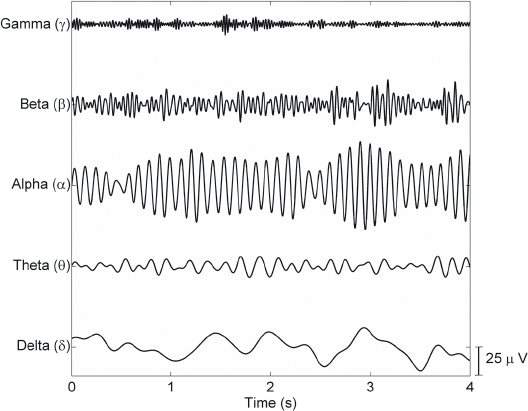
\includegraphics[width=1.2\textwidth]{aktywnosc.png}}%
	\caption{Wykresy pięciu rodzajów aktywności mózgu \cite{campisi}.}
\end{figure}

Fale beta są to fale z przedziału 13 Hz - 30 Hz. Aktywność blisko dolnej granicy pasma beta występuje w stanie czuwania, szczególnie podczas koncentracji uwagi i aktywnego myślenia. Fale beta o wyższej częstotliwości kojarzone są ze stanami lękowymi i umysłowym wzburzeniem. 

Ostatni rodzaj aktywności mózgu to fale gamma. Jako dolną granicę pasma częstotliwości, w której występuje ten rodzaj aktywności przyjmuje się od 25 Hz do 30 Hz. Wartość górnej granicy przyjmuje się jako 100 Hz. Fale gamma ze względu na wysoką częstotliwość i niską amplitudę zostały zaobserwowane jako ostatnie. Ponadto były one kiedyś uważane przez niektórych naukowców za artefakty pomiarowe, nie mające nic wspólnego z aktywnością mózgu. Współczesne badania sugerują, że aktywność w paśmie gamma ma związek z przetwarzaniem wrażeń sensorycznych, w szczególoności wizualnych \cite{swettenham} \cite{jia}.

\section{Kask Emotiv EPOC+}
Kask Emotiv EPOC+ (pokazany na rysunku 1.5) jest komercyjnym systemem zaprojektowanym do przeprowadzania badań z zastosowaniem elektroencefalografii. Emotiv EPOC+ posiada 14 elektrod rozmieszczonych w systemie 10\%, o oznaczeniach AF3, F7, F3, FC5, T7, P7, O1, O2, P8, T8, FC6, F4, F8, AF4. Dodatkowo posiada również elektrody P3 i P4 pełniące rolę elektrod referencyjnych. Kask wyposażony jest w elektrody chlorosrebrowe z filcowymi podkładkami, które przed rozpoczęciem badania należy nasączyć roztworem soli \cite{emotiv2}.

System wyposażony jest w 16-bitowy przetwornik analogowo-cyfrowy próbkujący sygnały z częstotliwością 2048 Hz. Spróbkowany sygnał jest następnie decymowany do częstotliwości próbkowania 128 Hz lub 256 Hz. Dwa najmłodsze bity każdej próbki są odrzucane - każda próbka ma więc rozdzielczość 14 bitów, a wartość jej najmłodszego bitu wynosi 0.51 \si{\micro\volt} \cite{emotiv} \cite{emotiv2}. 

Emotiv EPOC+ wyposażony jest w szereg filtrów cyfrowych. Są to: pasmowo-przepustowy filtr piątego rzędu o paśmie przenoszenia 0.2 Hz - 45 Hz oraz dwa cyfrowe filtry pasmowo-zaporowe o częstotliwościach środkowych odpowiedno 50 Hz i 60 Hz. Filtry pasmowo-zaporowe służą do eliminacji zakłóceń pochodzących z sieci energetycznej. Emotiv EPOC+ jest sprzężony zmiennoprądowo. Oznacza to, że składowa stała jest eliminowana z napięcia wejściowego \cite{emotiv} \cite{emotiv2}.
\begin{figure}[H]
	\centering
	\makebox[\textwidth][c]{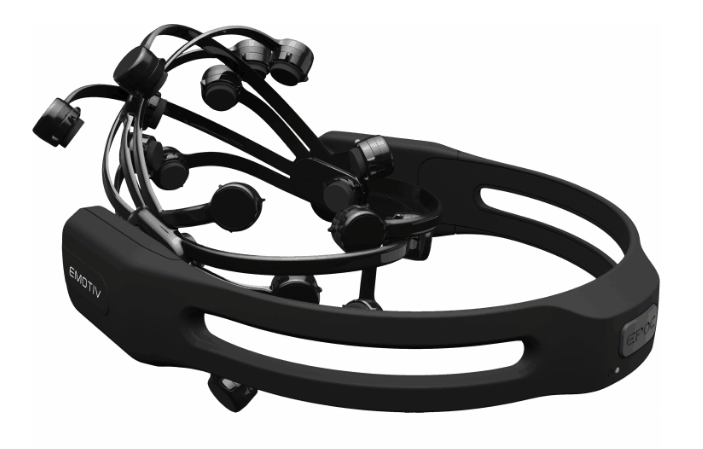
\includegraphics[width=0.6\textwidth]{emotivepoc.png}}%
	\caption{Kask Emotiv EPOC+ \cite{emotiv}}
\end{figure}

\chapter{Eliminacja artefaktów}
Rejestrowane sygnały elektroencefalograficzne prawie zawsze zanieczyszczone są różnego rodzaju artefaktami. Pochodzą one przede wszystkim z aktywności mięśni: poruszania kończynami, powiekami, gałkami ocznymi czy językiem. Bicie serca i praca układu oddechowego również zanieczyszczają elektroencefalogram \cite{uriguen}. Innymi rodzajami artefaktów są zakłócenia pochodzenia zewnętrznego: szum sieci energetycznej oraz dryft sygnału. Z tego powodu zazwyczaj wstępnie przetwarza się sygnał elektroencefalograficzny. Szum sieci energetycznej (wraz z jego harmonicznymi) możliwy jest do usunięcia za pomocą filtracji pasmowo-przepustowej. Dryft sygnału można wyeliminować za pomocą filtracji górnoprzepustowej. Do eliminacji pozostałych artefaktów często używana jest metoda zwana analizą składowych niezależnych \cite{uriguen}. 
\section{Analiza składowych niezależnych}
Analiza składowych niezależnych (ang. \textit{Independent Component Analysis, ICA}) jest to metoda rozwiązywania problemu ślepej separacji źródeł. Niech $\mathbf{s} = \left[s_1,...,s_n\right]$ oznacza $n$ sygnałów źródłowych niedostępnych dla obserwatora, a $\mathbf{x} = \left[x_1,...,x_n\right]$ oznacza $n$ sygnałów powstałych z liniowej kombinacji sygnałów $s_{1...n}$. Sygnał $x_i$ można przedstawić jako \cite{oja} \cite{langlois}:
\begin{equation}
x_i = a_{i1}s_1 + a_{i2}s_2 + ... + a_{in}s_n
\end{equation}
gdzie $a_{i1...n}$ są pewnymi nieznanymi współczynnikami. Zachodzi wtedy:
\begin{equation}
\mathbf{x} = \mathbf{As}
\end{equation}
gdzie $\mathbf{A}$ jest macierzą współczynników $a_{ij}$. Zadanie ślepej separacji źródeł polega na znalezieniu takiej macierzy $\mathbf{W} = \mathbf{A}^{-1}$ dla której zachodzi:
\begin{equation}
\mathbf{s} = \mathbf{Wx}
\end{equation}

Problem można przedstawić bardziej intuicyjnie: w pomieszczeniu znajduje się $n$ nieruchomych osób mówiących w tym samym momencie. W tym samym pomieszczeniu umiejscowionych jest $n$ mikrofonów nagrywających rozmowy. W takim przypadku problem ślepej separacji źródeł polega na tym, aby zarejestrowane sygnały przekształcić w nowy zestaw sygnałów tak, aby każdy sygnał zawierał zarejestrowaną mowę tylko jednej osoby (innej dla każdego sygnału) \cite{oja} \cite{langlois}.

W analizie składowych niezależnych zakłada się, że \cite{oja} \cite{langlois}:
\begin{itemize}
	\item sygnały źródłowe $s_{1...n}$ mają niegaussowskie funkcje gęstości prawdopodobieństwa $p(s_{1...n})$, 
	\item dowolna para sygnałów źródłowych $s_i$,$s_j$ jest niezależna:
	\begin{equation}
	p(s_i,s_j) = p(s_i)p(s_j)
	\end{equation}  
\end{itemize}
Zgodnie z centralnym twierdzeniem granicznym rozkład prawdopodobieństwa sumy niezależnych zmiennych losowych o jednakowych rozkładach prawdopodobieństwa, wartości oczekiwanej i wariancji zbiega do rozkładu normalnego. Analiza składowych niezależnych oparta jest na założeniu, że dowolny sygnał losowy $x_i$ ma rozkład prawdopodobieństwa bardziej zbliżony do normalnego niż którykolwkiek z sygnałów źródłowych $s_{1...n}$. W związku z tym wiersz $w_i$ macierzy $\mathbf{W}$ dobiera się tak, aby rozkład prawdopodobieństwa $\mathbf{w}^{T}_{i}\mathbf{x}$ był możliwie najbardziej oddalony od normalnego \cite{oja}. 

W roli miary oddalenia rozkładu prawdopodobieństwa od rozkładu normalnego można przyjąć wartość bezwzględną kurtozy \cite{oja}:
\begin{equation}
kurtosis(x) = E\{x^4\} - 3(E\{x^2\})^2
\end{equation}
Inną możliwą do zastosowania funkcją jest negentropia \cite{oja} \cite{langlois}:
\begin{equation}
negentropy(x) = H(x_{gauss}) - H(x)
\end{equation}
gdzie $H(x)$ jest entropią różnicową zmiennej losowej $x$:
\begin{equation}
H(x) = -\int p(x)\log p(x)dx
\end{equation}
natomiast $x_{gauss}$ jest zmienną losową o rozkładzie normalnym i macierzy kowariancji identycznej do macierzy kowariancji sygnału $x$. Innym podejściem do analizy składowych niezależnych jest minimalizacja funkcji informacji wzajemnej  \cite{oja} \cite{langlois}:
\begin{equation}
I(\mathbf{x}) = \sum_{i=1}^{n}H(x_i)-H(\mathbf{x})
\end{equation}

Istnieje wiele różnych implementacji analizy składowych niezależnych. Różnią się one funkcją miary oddalenia rozkładu prawdopodobieństwa od rozkładu normalnego, a takżę metodą optymalizacji. Przykładowe implementacje, to m.in.: FastICA \cite{oja}, InfoMax \cite{langlois}, AMICA \cite{palmer}, SOBI oraz JADE \cite{sahonero}.

Przed wykonaniem analizy elementów niezależnych zaleca się wstępne przetworzenie danych. Niezbędnym krokiem jest eliminacja składowej stałej z danych. Inna zalecana technika to wybielenie danych, czyli liniowe przekształcenie, w wyniku którego macierz kowariancji danych stanie się macierzą jednostkową. Opcjonalnie można też dokonać redukcji wymiarowości, na przykład poprzez analizę składowych głównych (ang. \textit{Principal Component Analysis, PCA}) \cite{oja}.

\chapter{Analiza sygnałów}
\section{Widmowa gęstość mocy}
Widmowa gęstość mocy (ang. \textit{Power Spectral Density, PSD}) sygnału $y(t)$ definiowana jest następująco \cite{stoica}:
\begin{equation}
P(\omega) = \sum_{k=-\infty}^{\infty}r(k)e^{-j\omega k}
\end{equation}
gdzie $\omega$ oznacza pulsację, $j$ oznacza jednostkę urojoną, natomiast $r(k)$ oznacza autokowariancję sygnału $y(n)$, definiowaną jako \cite{stoica}:
\begin{equation}
r(k) = E[y(n)y^*(n-k)]
\end{equation}
gdzie operator $*$ oznacza sprzężenie zespolone. Ze względu na to, że w praktyce dysponuje się tylko ograniczoną liczbą próbek sygnału $y(n)$, widmową gęstość mocy przybliża się następującą zależnością \cite{stoica}:
\begin{equation}
\hat{P}(\omega) = \frac{1}{N}\left|\sum_{n=1}^{N}y(n)e^{-j\omega n}\right|^2
\end{equation}
Metoda ta nazywana jest periodogramem. Periodogram jest estymatorem asymptotycznie nieobciążonym - wraz ze zwiększaniem liczby próbek sygnału obciążenie estymatora dąży do zera.

Jedną z najbardziej popularnych metod szacowania widmowej gęstości mocy jest oparta na periodogramie metoda Welcha \cite{welch}. W metodzie Welcha sygnał $y(n)$ o długości $N$ dzielony jest na $K$ ramek o długości $L = \frac{N}{K}$. Ramki przesuwane są o długość $D$ i mogą na siebie zachodzić. Każda ramka przepuszczana jest przez wybraną funkcję okna $w(n)$. Dla każdej ramki liczony jest oddzielny periodogram. Tak obliczone periodogramy są uśredniane. Metoda Welcha opisana jest wzorem:
\begin{equation}
\hat{P}_{welch}(\omega) = \frac{1}{KLU}\sum_{i=1}^{K}\left|\sum_{n=1}^{L}w(n)y\left(n+\left(i-1\right)D\right)e^{-j\omega n} \right|^2
\end{equation} 
gdzie $U$ jest mocą funkcji okna:
\begin{equation}
U = \frac{1}{L}\sum_{n=1}^{L}|w(n)|^2
\end{equation}
Dobór liczby ramek jest kompromisem pomiędzy wariancją estymatora a rozdzielczością częstotliwościową. Dzielenie sygnału na większą liczbę ramek może spowodać zmniejszenie wariancji estymatora, ale jednocześnie pogarsza rozdzielczość \cite{welch}. Metoda Welcha jest, tak jak standardowy periodogram, estymatorem asymptotycznie nieobciążonym, co oznacza, że wraz ze zwiększaniem długości sygnału $N$ obciążenie estymatora zbiega do zera \cite{stoica}.
\section{Modelowanie autoregresyjne}
Modelowanie autoregresyjne (ang. \textit{autoregressive modelling, AR modelling}) jest parametryczną metodą analizy sygnału. Zakłada się, że $n$-tą próbkę szeregu czasowego $x_i$ można aproksymować ważoną sumą $p$ poprzednich próbek \cite{pardey}.
\begin{equation}
\hat{x}_n = -\sum_{i=1}^{p}a_ix_{n-i}
\end{equation}
Parametr $p$ nazywany jest rzędem modelu AR i jest przyjmowany \textit{a priori}, przy czym rząd modelu powinien być dużo mniejszy niż długość serii danych $N$. Współczynniki $a_{1...p}$ są parametrami modelu AR, które należy obliczyć. Poniżej opisane zostaną dwie metody obliczania parametrów modelu AR: metoda autokorelacyjna oraz metoda maksymalnej entropii.

W metodzie autokorelacyjnej obliczanie parametrów modelu AR sprowadza się do znalezienia takiego zestawu parametrów, który zminimalizuje wartość średniej mocy błędu predykcji $E$, danej równaniem \cite{pardey}:
\begin{equation}
E = \frac{1}{N}\sum_{n=1}^{N}\left(x_n + \sum_{i=1}^{p}a_ix_{n-i}\right)^2
\end{equation}
Zakłada się, że próbki przed $x_1$ mają wartość zerową. Obliczenie pochodnych wyrażenia (3.7) po każdym ze współczynników $a_{1...p}$ i przyrównanie ich od zera
\begin{equation}
\frac{\partial E}{\partial a_i} = 0, \qquad 1 \le i \le p
\end{equation}
tworzy układ $p$ równań i $p$ niewiadomych.
\begin{equation}
\sum_{i=1}^{p}\left(\frac{1}{N}\sum_{n=1}^{N}x_{n-i}x_{n-j}\right)a_i = -\left(\frac{1}{N}\sum_{n=1}^{N}x_nx_{n-j} \right),\qquad 1 \le j \le p
\end{equation}
Po wyznaczeniu z układu równań (3.9) wyrażeń na $a_{1...p}$ i wstawieniu ich do równania (3.7) otrzymywane jest równanie (3.10), opisujące minimalną moc błędu predykcji.
\begin{equation}
E_p = \left(\frac{1}{N}\sum_{n=1}^{N}x_{n}^{2}\right) + \sum_{i=1}^{p}\left( \frac{1}{N}\sum_{n=1}^{N}x_nx_{n-i}\right)a_i
\end{equation}
Funkcja autokorelacji nieskończonego sygnału dana jest równaniem:
\begin{equation}
R_i = \lim\limits_{N \rightarrow \infty} \frac{1}{N}\sum_{n=1}^{N}x_nx_{n-i}, \qquad -\infty<i<\infty
\end{equation}
Wyrażenia w nawiasach z równania (3.10) są więc przybliżeniami $R_{0...p}$ obliczonymi na podstawie skończonego sygnału $x_{1...N}$. Zakłada się, że próbki przed $x_1$ są równe zero. Jeżeli sygnał jest stacjonarny, to $R_i = R_{-i}$, wtedy zachodzi:
\begin{equation}
\tilde{R}_{|i-j|} = \frac{1}{N}\sum_{n=1}^{N}x_{n-i}x_{n-j}, \quad 0 \le i \le p, \quad 1 \le j \le p
\end{equation}
Po wstawieniu wyrażeń na $\tilde{R}_0,...,\tilde{R}_p$ do układu równań (3.9), otrzymywane są równania Yule-Walkera.
\begin{equation}
\begin{bmatrix}
\tilde{R}_0 & \tilde{R}_1 & \tilde{R}_2 & ... & \tilde{R}_p \\
\tilde{R}_1 & \tilde{R}_0 & \tilde{R}_1 & ... & \tilde{R}_{p-1} \\
\tilde{R}_2 & \tilde{R}_1 & \tilde{R}_0 & ... & \tilde{R}_{p-2} \\
\vdots & \vdots & \vdots & \ddots & \vdots \\
\tilde{R}_p & \tilde{R}_{p-1} & \tilde{R}_{p-2} & ... & \tilde{R}_0 \\
\end{bmatrix}
\begin{bmatrix}
1 \\ a_1 \\ a_2 \\ \vdots \\ a_p
\end{bmatrix} = 
\begin{bmatrix}
E_p \\ 0 \\ 0 \\ \vdots \\ 0
\end{bmatrix}
\end{equation}
Współczynniki $a_{1...p}$ mogą być obliczone w wydajny sposób za pomocą algorytmu Levinsona-Durbina, który rekursywnie rozwiązuje równania Yule-Walkera dla modeli rzędu od $m=0$ do $m=p$ \cite{pardey} \cite{stoica}. 

Metoda maksymalnej entropii jest modyfikacją metody autokorelacji. Wyrażenie na średni błąd predykcji z równania (3.7) jest modyfikowane w taki sposób, aby uwzględnić również błąd predykcji wstecznej, czyli błąd predykcji danej próbki na podstawie $p$ przyszłych próbek. Ograniczana jest również liczba próbek, na podstawie których obliczana jest średnia wartość błędu predykcji - w taki sposób aby nie korzystać w obliczeniach z próbek wcześniejszych niż $x_1$ i późniejszych niż $x_N$. W ten sposób można zrezygnować z założenia o zerowej wartości tych próbek. Zmodyfikowane wyrażenie na średnią wartość błędu predykcji dane jest równaniem (3.14).
\begin{equation}
\begin{split}
E = \frac{1}{2(N-p)}\sum_{n=p+1}^{N}\left[\left(x_n + \sum_{i=1}^{p}a_ix_{n-i}\right)^2 + \left(x_{n-p} + \sum_{i=1}^{p}a_ix_{n-p+i}  \right)^2\right]
\end{split}
\end{equation}
Wartość równania (3.14) minimalizuje się w sposób analogiczny do pokazanego w przypadku metody autokorelacyjnej. Wartości współczynników $a_{1...p}$ można wtedy obliczyć algorytmem Burga, który dodatkowo w rekursywny sposób oblicza błędy predykcji przedniej i wstecznej.

Na podstawie obliczonego modelu autoregresyjnego można obliczyć estymatę widmowej gęstości mocy za pomocą wzoru \cite{pardey}:
\begin{equation}
\tilde{P}(\omega) = \frac{E_pT_s}{|1+\sum_{i=1}^{p}a_ie^{-ij\omega T_s}|^2}
\end{equation}
gdzie $T_s$ oznacza okres próbkowania. Modelowanie autoregresyjne dobrze sprawdza się w modelowaniu sygnałów, których widma charakteryzują się wysokimi, wąskimi wierzchołkami. Analogiczną metodą są modele ze średnią ruchomą (ang. \textit{moving average, MA}), które dobrze się sprawdzają w przypadku sygnałów, których widma charakteryzują się wąskimi dolinami. Jest to jednak metoda mniej popularna, gdyż wymaga rozwiązania układu równań nieliniowych. Uogólnieniem obu metod są modele ARMA \cite{pardey} \cite{stoica}. 
 

\section{Dyskretna transformacja falkowa}
Transformacja falkowa funkcji $x(t)$ jest transformacją postaci \cite{addison}:
\begin{equation}
w(a,b) = \frac{1}{\sqrt{a}}\int_{-\infty}^{\infty}x(t)\psi^*(\frac{t-b}{a})dt
\end{equation}
gdzie $\psi(t)$ jest dowolną falką, $a > 0$ oznacza parametr skali, a $b$ oznacza przesunięcie. Falka jest to rodzaj oscylującej funkcji o skończonej energii i zerowej wartości średniej, której amplituda początkowo ma wartość zerową, rośnie do maksimum, a następnie ponownie opada do zera. Mówiąc prościej, falka jest to tymczasowa oscylacja. Obliczenie splotu sygnału z falką o określonej częstotliwości pozwala określić nie tylko czy w danym sygnale występuje składowa o danej częstotliwości, ale również - w przeciwieństwie do transformacji Fouriera - określić moment czasu, w którym dana składowa występuje. Z tego powodu falki znajdują zastosowanie w analizie artefaktów, stanów przejściowych oraz detekcji zmian w sygnałach \cite{addison}. 

Rodzina funkcji falkowych budowana jest na podstawie falki-matki $\psi(t)$ poprzez skalowanie parametrem $a$, przesunięcie parametrem $b$ oraz normalizację. 
\begin{equation}
\psi_{a,b}(t) = \frac{1}{\sqrt{a}}\psi(\frac{t-b}{a})
\end{equation} 
Ze względu na to, że całka z równania (3.16) jest w praktyce niemożliwa do obliczenia dla ciągłych wartości $a$ oraz $b$, wykorzystuje się dyskretną transformację falkową (ang. \textit{Discrete Wavelet Transform, DWT}) dla której wartości parametrów $a,b$ przyjmują wartości dyskretne. Najczęściej przyjmuje się $a = 2^m$, $b = k2^m$ dla $k,m \in \mathbb{N}$. Zachodzi wtedy \cite{addison}:
\begin{equation}
\psi_{m,k}(t) = \frac{1}{\sqrt{2^m}}\psi(2^{-m}t-k)
\end{equation}

Parametr skali $a$ decyduje o paśmie częstotliwości falki, zarówno jego szerokości, jak i częstotliwości środkowej. Zwiększanie wartości parametru skali rozciąga falkę, zawęża jej widmo i jednocześnie przesuwa je w kierunku niższych częstotliwości. Po lewej stronie rysunku 3.1 przedstawiono wpływ parametru skali (ang. \textit{dilation}) na funkcję falkową (ang. \textit{wavelet function}) $h(t) = (e^{j\pi t} - e^{j\pi t/2})/(j\pi t/2)$ w dziedzinie czasu (ang. \text{time}). Po prawej stronie przedstawiono wpływ parametru skali na estymowane widmo falki (ang. \textit{spectrum estimation}). Częstotliwość (ang. \textit{frequency}) wyrażono w stosunku do częstotliwości próbkowania. W przypadku, gdy $a = 1,2,4,...$ każda kolejna falka ma dwukrotnie węższe pasmo przenoszenia i dwukrotnie niższą częstotliwość środkową pasma przenoszenia. Stanowi to jednocześnie kompromis pomiędzy rozdzielczością czasową i częstotliwościową. Krótsze falki, odpowiadające wyższym częstotliwościom, pozwalają na dokładniejszą lokalizacje czasową oscylacji, ale nie pozwalają dokładnie określić częstotliwości. Dłuższe falki pozwalają dokładniej określić częstotliwość oscylacji, ale nie pozwalają dokładnie określić momentu czasu jej wystąpienia. 
\begin{figure}[H]
	\centering
	\makebox[\textwidth][c]{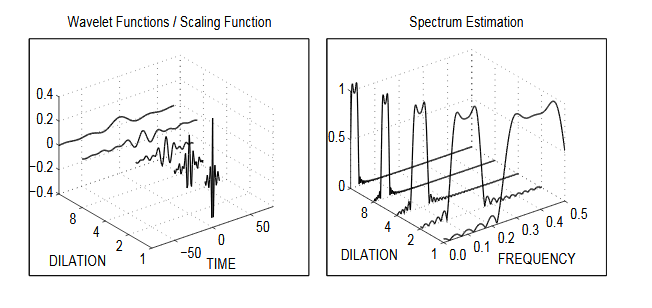
\includegraphics[width=1.1\textwidth]{wavscaling.png}}%
	\caption{Część rzeczywista falki $h(t) = (e^{j\pi t} - e^{j\pi t/2})/(j\pi t/2)$ skalowana wartościami parametru skali $a=1,2,4,8,16$ (lewa strona). Wpływ parametru skali $a$ na aproksymowane widmo falki (prawa strona) (\textit{wavelet function} - funkcja falkowa, \textit{spectrum estimation} - estymacja widma, \textit{time} - czas, \textit{dilation} - parametr skali, \textit{frequency} - częstotliwość) \cite{prochazka}}
\end{figure}
Ze względu na to, że pokrycie pełnego pasma częstotliwości wymagałoby zastosowania nieskończonej liczby falek, wprowadza się funkcję skalujacą $\phi$, dopasowaną do rodziny falek. Funkcja skalująca, w przeciwieństwie do funkcji falkowej, ma niezerową wartość średnią i dolnoprzepustową charakterystykę częstotliwościową. Tym samym możliwe jest pokrycie pełnego pasma częstotliwości za pomocą dowolnej, skończonej liczby falek oraz funkcji skalującej.

Dyskretna transformacja falkowa może być obliczona w wydajny sposób za pomocą pary komplementarnych filtrów: dolnoprzepustowego $g$ oraz górnoprzepustowego $h$. Sygnał wejściowy jest podawany równolegle do obu filtrów - tym samym jest on rozkładany na dwie składowe: niskoczęstotliwościową oraz wysokoczęstotliwościową. Z obydwu składowych wyrzucana jest co druga próbka. Tak otrzymane składowe nazywane są w literaturze anglojęzycznej odpowiednio \textit{approximation} oraz \textit{detail}. Składowa niskoczęstotliwościowa może być dalej rozkładana według tego samego schematu powtórzonego wybraną liczbę razy. Schemat obliczania DWT za pomocą zespołu filtrów przedstawiono na rysunku 3.2.
\begin{figure}[H]
	\centering
	\makebox[\textwidth][c]{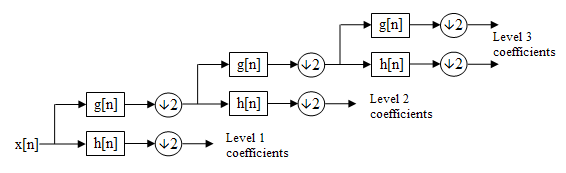
\includegraphics[width=1.2\textwidth]{dwttree.png}}%
	\caption{Schemat obliczania 3-poziomowej dyskretnej transformaty falkowej za pomocą pary komplementarnych filtrów: dolnoprzepustowego $g$ oraz górnoprzepustowego $h$. W podanym przykładzie sygnał jest rozkładany na cztery podpasma \cite{dwttree}}
\end{figure}
\chapter{Klasyfikacja}
\section{Zadanie klasyfikacji}

Zadanie klasyfikacji polega na przyporządkowaniu \textit{n}-wymiarowego punktu pomiarowego do jednej z \textit{k} klas. Zadanie klasyfikacji jest jednym z dwóch rodzajów zadań predykcyjnych spotykanych w dziedzinie uczenia statystycznego - drugim rodzajem zadania jest regresja. Uczenie statystyczne jest działem nauki zajmującym się tworzeniem modeli na podstawie danych pomiarowych. Celem tworzenia modeli jest uzyskanie możliwości predykcji wartości wyjściowej (zwaną również odpowiedzią lub zmienną zależną) na podstawie wektora wartości wejściowych (zwanych również pobudzeniami, cechami, predyktorami lub zmiennymi niezależnymi) \cite{prml} \cite{islr} \cite{eslii}.

Zadanie klasyfikacji różni się od zadania regresji tym, że w zadaniu regresji zmienna wyjściowa jest zmienną ilościową, natomiast w zadaniu klasyfikacji zmienna wyjściowa jest zmienną jakościową (kategoryczną). Zmienne ilościowe to zmienne, które są mierzalne i które można wyrazić za pomocą liczb. Przykładami zmiennej ilościowej są wzrost czy waga człowieka. Zmiennymi jakościowymi mogą być kolor oczu, grupa krwi, rodzaj znaku drogowego czy wystąpienie zawału u pacjenta  \cite{islr} \cite{eslii}. 

Przykładem zadania klasyfikacji jest przewidywanie wczesnej umieralności pacjentów z chorobami serca na podstawie czynników ryzyka. Zbiorem klas może wtedy być \textit{niskie ryzyko}, \textit{średnie ryzyko}, \textit{wysokie ryzyko} \cite{nashef}. Innym przykładem jest rozpoznawanie obecności guza mózgu ze zdjęć rentgenowskich - wtedy zbiór klas może być binarny (obecność guza lub brak guza). Przykładem zadania regresji może być szacowanie liczby godzin pobytu pacjenta na oddziale ratunkowym na podstawie takich zmiennych, jak liczba pacjentów czy konieczność wykonania zdjęć rengenowskich \cite{combes}.

Zmienne jakościowe w ogólności nie są wyrażalne liczbowo w intuicyjny sposób, ale na potrzeby przetwarzania komputerowego kategorie najczęściej odwzorowuje się np. poprzez przyporządkowywanie im kolejnych liczb naturalnych. Taka metoda ma jednak swoje wady. Jako przykład można rozważyć model statystyczny mający przyporządkowywać pacjentów do jednej z trzech kategorii chorobowych: \textit{zawał}, \textit{przedawkowanie leków}, \textit{wstrząs epileptyczny}. Wtedy kategorię \textit{zawał} można zakodować za pomocą liczby 1, kategorię \textit{przedawkowanie leków} za pomocą liczby 2, a kategorię \textit{wstrząs epileptyczny} za pomocą liczby 3. Zastosowanie praw arytmetyki do tak zakodowanych kategorii sugeruje,  że kategoria \textit{przedawkowanie leków} jest wartością pośrednią pomiędzy kategoriami \textit{zawał} i \textit{wstrząs epileptyczny}, co jest błędnym wnioskiem. Ten sposób interpretacji może mieć sens, jeżeli kategorie w danym problemie są uszeregowane (np. \textit{mały},\textit{średni},\textit{duży}), w ogólnym przypadku tak jednak nie jest \cite{islr}. Innym sposobem kodowania jest przyporządkowywanie każdej z \textit{k} kategorii wektora o długości \textit{k} mającego wartość 1 na dokładnie jednej pozycji (innej dla każdej kategorii) i wartości 0 na wszystkich innych (ang. \textit{dummy variables}, \textit{one-hot encoding}). Wtedy kategorie z powyżej podanego przykładu można zakodować następująco \cite{garavaglia} \cite{islr} \cite{potdar}: 
\begin{equation*}
\begin{blockarray}{*{6}{c}}
\begin{block}{*{6}{c}}
\hbox{\textit{zawał}}     &  [ & 1 & 0 & 0 & ] \\
\hbox{\textit{przedawkowanie leków}}     &  [ & 0 & 1 & 0 & ] \\
\hbox{\textit{wstrząs epileptyczny}} &  [ & 0 & 0 & 1 & ] \\
\end{block}
\end{blockarray}
\end{equation*}

Aby zbudować model, należy wybrać technikę modelowania danych - lub kilka, jeżeli celem jest porównanie ich skuteczności. Niektóre techniki nadają się zarówno do modelowania regresyjnego, jak i klasyfikacyjnego. Inne są dedykowane tylko dla jednego typu zadania. W zadaniu klasyfikacji zarówno metodę modelowania danych, jak i opracowany model często nazywamy klasyfikatorem. 

Po wybraniu technik modelowania dostępny zbiór danych należy podzielić na trzy podzbiory: zbiór danych uczących, zbiór danych testowych oraz zbiór danych walidacyjnych. We wszystkich tych podzbiorach każda obserwacja powinna składać się z wektora zmiennych niezależnych (cech, predyktorów, pobudzeń) oraz ze zmiennej zależnej (odpowiedzi). Według autorów pracy \cite{eslii} domyślnie zaleca się użyć 50\% dostępnych danych w roli danych uczących oraz po 25\% jako dane walidacyjne i testowe, ale często te proporcje przyjmują odpowiednio wielkości: 70\%, 10\% i 20\%. 

Dane uczące służą do wyznaczania takich wartości parametrów modelu, aby w odpowiedzi na podane dane model zwrócił poprawną wartość wyjściową (lub zbliżoną w przypadku regresji). Proces ten nazywany jest uczeniem. Jeżeli model nie jest w stanie nauczyć się poprawnego reagowania na pobudzenia ze zbioru danych uczących z pożądaną skutecznością, to może to oznaczać, że zastosowany zbiór danych uczących jest za mały. Zjawisko to nazywane jest niedostatecznym dopasowaniem czy też niedouczeniem modelu (ang. \textit{underfitting}). Może to również oznaczać konieczność wyboru innej techniki modelowania. 

Zbiór danych testowych wykorzystywany jest do sprawdzenia jak wyuczony model radzi sobie z predykcją obserwacji niewykorzystanych w procesie uczenia.
Do oceny skuteczności przeprowadzonego procesu uczenia służy funkcja błędu, która ilościowo wyraża całkowity błąd predykcji dla danego zbioru danych. W zadaniu regresji najczęściej spotykaną funkcją błędu jest błąd średniokwadratowy (ang. \textit{mean squared error}, \textit{MSE}), będący średnią wartością kwadratu różnicy pomiędzy wartością prawdziwą $y_i$ i predykowaną $\hat{y}_i$ ze wszystkich $N$ obserwacji w zbiorze danych. 
\begin{equation}
MSE = \frac{1}{N}\sum_{i}^{N}(y_i - \hat{y}_i)^2
\end{equation}
W przypadku zadania klasyfikacji do oceny całkowitego błędu klasyfikacji używa się stosunku liczby niepoprawnie zaklasyfikowaych obserwacji do liczby wszystkich obserwacji. (Oznaczenia we wzorze (4.2) jak wyżej):
\begin{equation}
\frac{1}{N}\sum_{i=1}^{N}I(y_i \neq \hat{y}_i) 
\end{equation}


Jeżeli skuteczność predykcji danych testowych jest dużo niższa niż danych treningowych, to może to oznaczać, że użyty zbiór danych uczących był za mały. W przypadku predykcji obserwacji pochodzących z sensorów może to oznaczać również znaczne zaszumienie danych, co oznacza konieczność zastosowania dodatkowych metod przetwarzania wstępnego w celu ich odszumienia. Ostatecznie, niska skuteczność predykcji danych testowych może również być objawem nadmiernego dopasowania czy też przeuczenia \textit{(ang. overfitting}) modelu - szczególnie, jeżeli jednocześnie wartość błędu treningowego jest niska. 

Zjawisko przeuczenia najłatwiej wyjaśnić (zarówno matematycznie, jak i intuicyjnie) na przykładzie zadania regresji. W pracach \cite{islr} \cite{eslii} przyjmuje się, że proces generujący dane pomiarowe na podstawie których budowany jest model można zamodelować jako:
\begin{equation}
Y = f(X) + \epsilon
\end{equation}
gdzie $Y$ jest zmienną zależną obserwacji, $X$ jest $n$-wymiarowym wektorem cech obserwacji, $f(X)$ jest pewną nieznaną funkcją $X$, natomiast $\epsilon$ jest losowym błędem, niezależnym od $X$, o zerowej wartości średniej. Błąd ten wynika z parametrów, których nie można zaobserwować lub które są zbyt skomplikowane, aby je zamodelować. Zadaniem regresji jest wtedy znalezienie funkcji (nazywanej funkcją estymującą):
\begin{equation}
\hat{Y} = \hat{f}(X)
\end{equation}
która będzie przybliżać nieznaną funkcję $f(X)$. Zjawisko przeuczenia następuje, gdy zbudowany model dopasowuje się nie tylko do estymowanej funkcji $f(X)$, ale także do konkretnych realizacji losowych błędów $\epsilon$ występujących w zbiorze danych uczących. W innym zbiorze obserwacji wygenerowanych przez ten sam proces wartości błędów $\epsilon$ dla tych samych wektorów cech $X$ mogą przyjmować zupełnie inne wartości. W takim przypadku mniej elastyczny model, mniej dokładnie dopasowujący się do danych uczących, okaże się bardziej dokładny. 

Wartość średnią błędu estymacji (czyli różnicy pomiędzy wartością pomierzoną i wartością przewidzianą na podstawie modelu) można wyrazić w postaci równania 4.4.
\begin{equation}
E(Y-\hat{Y})^2 = E[f(X) + \epsilon - \hat{f}(X)]^2 = [f(X) - \hat{f}(X)]^2 + Var(\epsilon)
\end{equation}

Składnik $[f(X) - f(\hat{x})]^2$ nazywany jest błędem redukowalnym, natomiast składnik $Var(\epsilon)$ - błędem nieredukowalnym. Błąd redukowalny można zminimalizować, dobierając odpowiednią technikę modelowania i dostarczając odpowiednio duży zbiór danych uczących. Na wartość błędu nieredukowalnego nie można wpłynąć, nawet gdyby prawdziwa postać estymowanej funkcji $f(X)$ była znana. Błąd nieredukowalny tym samym stanowi dolną granicę oczekiwanej wartości błędu estymacji. 

Według autorów pracy \cite{islr} równanie (4.4) można rozwinąć w równanie (4.5).

\begin{equation}
E(Y-\hat{Y})^2 = Var[\hat{f}(X)] + \big[Bias[\hat{f}(X)]\big]^2 + Var(\epsilon)
\end{equation}
Z równania (4.5) wynika, że błąd redukowalny z równania (4.4) można dalej zdekomponować na dwa czynniki: błąd wynikający z wariancji modelu i błąd wynikający z obciążenia (ang. \textit{bias}) modelu. Obciążenie modelu definiuje się jako różnica pomiędzy średnią wartością predykowaną przez model i średnią wartością danych generowanych przez proces \cite{prml} \cite{eslii} \cite{leborgne}.
\begin{equation}
Bias[\hat{f}(X)] = E[\hat{f}(X)] - E(Y)
\end{equation}
Obciążenie modelu wskazuje na tendencję predykowanych wartości do bycia zawyżonymi lub zaniżonymi (w zależności od znaku wartości obciążenia). Modele z niską wartością obciążenia typowo są modelami bardziej elastycznymi - są one w stanie odwzorować funkcje charakteryzujące się większą zmiennością. Elastyczność (lub złożoność) modelu często jest interpretowana jako liczba parametrów modelu - na przykład stopień wielomianu w regresji wielomianowej. Oznacza to, że obciążenie modelu wynika z czynienia założeń dotyczących procesu generującego dane, które ów proces upraszczają - na przykład podczas dopasowywania funkcji liniowej do danych wygenerowanych przez proces będący wielomianem wyższego rzędu \cite{islr}. 

Wariancja modelu jest z kolei definiowana jako oczekiwana wartość kwadratu różnicy wartości predykowanej i średniej wartości predykowanej \cite{prml} \cite{leborgne}.
\begin{equation}
Var[\hat{f}(X)] = E\big[\hat{f}(X) - E[\hat{f}(X)]\big]^2
\end{equation}
Im większa wartość wariancji, tym większy jest ''rozstrzał'' predykowanych wartości naokoło ich wartości oczekiwanej. Parametry modeli o wysokiej wariancji są wrażliwe na konkretne realizacje losowych błędów $\epsilon$ w zastosowanych danych uczących. Inaczej mówiąc, modele z wysoką wariancją wytrenowane za pomocą dwóch różnych zbiorów danych wygenerowanych przez ten sam proces mogą mieć kompletnie inne wartości parametrów. Modele niskowariancyjne (np. model liniowy) są na to zjawisko odporne, oczywiście przy założeniu, że wartość oczekiwana błędów losowych $\epsilon$ pozostaje równa 0. Modele z niższą wartością wariancji typowo są modelami mniej elastycznymi. 

Wraz z tym, jak zwiększana jest złożoność modelu maleje jego obciążenie i jednocześnie rośnie wariancja. W literaturze anglojęzycznej zjawisko to znane jest jako \textit{bias-variance tradeoff}, czyli kompromis pomiędzy obciążeniem i wariancją. Sugeruje to, że istnieje optymalna złożoność modelu, minimalizująca oczekiwaną wartość błędu estymacji. 

Doświadczenia empiryczne potwierdzają słuszność tego rozumowania. Na rysunku 4.1 przedstawiono w postaci wykresów wyniki eksperymentu opublikowanego w pracy Jamesa i in. \cite{islr}. Po lewej stronie przedstawiono wygenerowane komputerowo dane (czarne kropki), funkcję $f(X)$ procesu generującego dane (czarna krzywa) oraz trzy modele zbudowane na podstawie tych danych. Pomarańczową krzywą oznaczono model liniowy. Krzywymi niebieską i zieloną oznaczono modele oparte o wygładzone funkcje sklejane (ang. \textit{smoothing splines}). Po prawej stronie przedstawiono wykres zależności błędu uczenia (ang. \textit{learning error}) i błędu testowego (ang. \textit{test error}) od elastyczności modelu. Błąd uczenia oznacza łączny błąd popełniony podczas próby predykcji wartości obserwacji wykorzystanych w procesie uczenia. Z kolei błąd testowy odnosi się do łącznego błędu popełnionego podczas próby predykcji wartości obserwacji z pewnego zbioru niewykorzystanego w procesie uczenia.  Szara linia oznacza błąd uczenia, natomiast różową linią oznaczono błąd testowy (dane testowe nie zostały przedstawione na wykresie). Kolorowe kwadraty oznaczają konkretne wartości błędów uczenia i błędów testowych dla trzech modeli przedstawionych po lewej stronie.

Na wykresach widać, że zwiększanie elastyczności modelu zawsze powoduje spadek błędu uczenia, ale tylko do pewnego momentu powoduje spadek błędu testowego. Gdy elastyczność modelu jest większa niż dla punktu oznaczonego niebieskim kwadratem (minumum błędu testowego), to opracowany model zaczyna zbyt mocno dopasowywać się do wartości losowych błędów $\epsilon$ w generowanych danych, co ostatecznie pogarsza jego zdolność generalizacji, czyli poprawnej predykcji obserwacji nienapotkanych w procesie uczenia. Objawia się to wzrostem wartości błędu testowego.

Liniowy model przedstawiony na rysunku 4.1 charakteryzuje się dużą wartością zarówno błędu uczenia, jak i błędu testowego - jest on niedostatecznie dopasowany. Model oznaczony zieloną krzywą ma niską wartość błędu uczenia, ale wysoką wartość błędu testowego - jest on nadmiernie dopasowany. Model oznaczony niebieską krzywą ma wartość błędu testowego bliską minimum - jest on odpowiednio dopasowany. 

Należy zaznaczyć, że intepretacja złożoności modelu jako liczby parametrów nie zawsze jest słuszna, co jest pokazane w następnym podrozdziale dotyczącym klasyfikatora $k$-najbliższych sąsiadów (ang. \textit{k-nearest neighbours}, \textit{k-NN}). 
\begin{figure}[H]
	\centering
	\makebox[\textwidth][c]{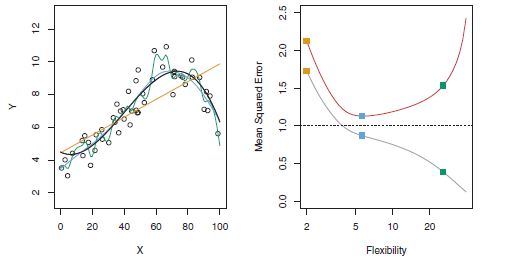
\includegraphics[width=1.2\textwidth]{learningerr.png}}%
	\caption{Czarnymi kropkami zaznaczono wygenerowane dane uczące. Czarną krzywą zaznaczono funkcję $f(X)$ procesu generującego dane. Zieloną, niebieską oraz pomarańczową krzywą zaznaczono trzy różne modele zbudowane na podstawie wygenerowanych danych (lewa strona). Wykres zależności błędu średniokwadratowego danych uczących (szara krzywa) i niezaprezentowanych danych testowych (różowa krzywa), wraz z zaznaczonymi wartościami tych błędów dla poszczególnych modeli (prawa strona) \cite{islr}}
\end{figure}

Zbiór danych walidacyjnych wykorzystywany jest w procesie uczenia do uniknięcia przeuczenia modelu. Pełni on podobną rolę, co zbiór danych testowych - służy do oceny zdolności modelu do poprawnej predykcji obserwacji nie napotkanych w procesie uczenia. Różnica jest taka, że błąd walidacji obliczany jest wielokrotnie w trakcie trwania procesu uczenia. Jeżeli wartość błędu walidacji zaczyna rosnąć, oznacza to, że należy przerwać proces uczenia aby zapobiec przeuczeniu modelu. 

Należy podkreślić, że system klasyfikujący nie musi być oparty na wyłącznie jednym klasyfikatorze - może on składać się z kilku klasyfikatorów. W takim wypadku ostateczny wynik wyznaczany jest przez głosowanie - obserwacja jest zaliczana do tej klasy, która została zwrócona jako wynik przez największą liczbę składowych klasyfikatorów. W pracy \cite{lan} opisany został system klasyfikacji sygnałów EEG oparty o 3 klasyfikatory: $k$-najbliższych sąsiadów, Gaussowski model mieszany oraz okno Parzena. Skuteczność klasyfikacji tak opracowanego systemu okazała się wyższa niż wszystkich składowych klasyfikatorów z osobna. O podobnych rozwiązaniach wspomniano w pracy \cite{lotte1}.

W teorii decyzji wykorzystuje się niekiedy pojęcie optymalnego klasyfikatora Bayesa. Jest to klasyfikator, który przyporządkowuje obserwacje $x_0$ do tej kategorii $j$, której prawdopodobieństwo warunkowe $P(Y = j|X = x_0)$ jest możliwie największe. Jeżeli za miarę błędu klasyfikacji użyje się średniej wartości niepoprawie zaklasyfikowanych obserwacji, to średni błąd popełniony przez ten klasyfikator (nazywany błędem Bayesa, ang. \textit{Bayes error rate}) jest możliwie najmniejszy, więc taki klasyfikator jest optymalny \cite{islr} \cite{eslii}. Oczywiście prawdopodobieństwo warunkowe przynależności obserwacji do danej klasy dla danych uzyskanych eksperymentalnie jest w ogólności nieznane, więc konstrukcja takiego klasyfikatora nie jest możliwa. Metody klasyfikacji używane w praktyce mają na celu możliwie najlepiej aproksymować klasyfikator Bayesa.

W dalszej części rozdziału zostaną zaprezentowane trzy popularne techniki klasyfikacji danych: metoda $k$-najbliższych sąsiadów, sieci neuronowe oraz maszyny wektorów nośnych. Wszystkie opisanej tutaj techniki zostały zastosowane w eksperymentalnej części pracy. 

\section{Metoda $k$-najbliższych sąsiadów}
Metoda $k$-najbliższych sąsiadów (ang. \textit{k-nearest neighbours}, $k$-NN) jest jedną z najstarszych i jednocześnie najprostszych metod klasyfikacji. Klasyfikator $k$-najbliższych sąsiadów wybiera $k$ obserwacji treningowych znajdujących się najbliżej, wedle obranej miary odległości, od podanej na wejście obserwacji testowej. Obserwacja ta jest następnie przyporządkowywana do kategorii występującej najczęściej wśród wybranych $k$ najbliższych obserwacji testowych. Metoda $k$-NN może być również użyta w zadaniach regresji. Odpowiedź modelu jest wtedy równa wartości średniej ze zmiennych zależnych $k$ najbliższych obserwacji treningowych \cite{islr} \cite{eslii}.

Klasyfikator $k$-NN wykorzystuje zbiór $k$ punktów testowych najbliższych do danej obserwacji testowej $x_0$, oznaczany jako $N_0$, do oszacowania prawdopodobieństwa warunkowego przynależności tej obserwacji testowej do danej klasy $j$ dla wszystkich możliwych klas \cite{islr}. Prawdopodobieństwo to jest obliczane jako stosunek liczby obserwacji $y_i \in N_0$ należących do klasy $j$ do liczby wszystkich rozpatrywanych obserwacji $k = |N_0|$. Obserwacja testowa $x_0$ ostatecznie jest przyporządkowywana do klasy mającej największe prawdopodobieństwo warunkowe. 
\begin{equation}
Pr(Y = j | X = x_0) = \frac{1}{k}\sum_{y_i\in N_0}I(y_i = j)
\end{equation}

Metoda $k$-NN jest czasami zaliczana do leniwych metod uczenia (ang. \textit{lazy learning}), gdyż odpowiedź klasyfikatora obliczana jest bezpośrednio na podstawie obserwacji uczących. W procesie uczenia klasyfikatora $k$-NN nie wykonuje się żadnych obliczeń - uczenie sprowadza się do zapamiętania obserwacji treningowych. Umożliwia to dodawanie nowych obserwacji treningowych w czasie działania systemu klasyfikacyjnego.

Stosując klasyfikator $k$-NN, należy wybrać miarę odległości pomiędzy obserwacjami. Zastosowania miara odległości powinna być metryką, czyli funkcją $d:M\times M \rightarrow [0,+\infty) $ zdefinowaną na zbiorze $M$, spełniającą dla dowolnych punktów $x,y,z \in M$ następujące warunki:
\begin{itemize}
	\item identyczność elementów nierozróżnialnych: $d(x,y) = 0 \iff x=y$,
	\item symetria: $d(x,y) = d(y,x)$,
	\item nierówność trójkąta: $d(x,z) <= d(x,y) + d(y,z)$.
\end{itemize}

Najczęściej stosowana jest odległość w przestrzeni $l^2$, znana również jako odległość Euklidesowa \cite{prasath}.
\begin{equation}
l_2(x,y) = \sqrt{\sum_{i=1}^{N}(x_i-y_i)^2}
\end{equation}
Inną możliwą do zastosowania miarą jest odległość w przestrzeni $l^1$ (nazywana również odległością Manhattan lub taksówkową) \cite{prasath}. 

\begin{equation}
l_1(x,y) = \sum_{i=1}^{N}|x_i-y_i|
\end{equation}
Obie powyższe miary odległości są szczególnymi przypadkami odległości Minkowskiego \cite{lu} \cite{prasath}.
\begin{equation}
l_m(x,y) = \left(\sum_{i=1}^{N}|x_i-y_i|^m\right)^{1/m}
\end{equation}

Możliwe jest również zastosowanie miary odległości nie będącej odległością Minkowskiego. W pracy Prasatha i in. porównano skuteczność klasyfikacji danych z różnych zbiorów z zastosowaniem metody $k$-NN z 52 różnymi metodami pomiaru odległości \cite{prasath}. Uwzględniono również wartość parametru $k$ oraz poziom szumów pomiarowych. W przeprowadzonym eksperymencie zastosowanie pewnych miar odległości w ogólności skutkowało wyższą skutecznością klasyfikacji. Zastosowanie miary $l^1$ skutkowało nieco wyższą skutecznością klasyfikacji niż zastosowanie miary $l^2$, aczkolwiek różnica była niewielka. Najlepsze rezultaty uzyskano przy zastosowaniu miary Hassanata, zaproponowanej w 2014 roku \cite{hassanat}.

Kluczową kwestią w zapewnianiu skuteczności klasyfikatora $k$-NN jest wybór wartości parametru $k$. Parametr $k$ można interpretować jako przywołaną w poprzednim rozdziale złożoność modelu. Niska wartość parametru $k$ powoduje, że klasyfikator jest podatny na wpływ szumu i obserwacji odstających. Zbyt wysoka wartość parametru $k$ powoduje zbyt duży wpływ względnie mocno oddalonych obserwacji treningowych. Rozwiązaniem tego problemu może być zastosowanie ważonego algorytmu $k$-NN. W takim wariancie algorytmu każda z $k$ najbliższych obserwacji treningowych oddaje głos na klasę, do której należy, przy czym każdy taki głos ma wagę, która jest tym wyższa, im bliżej dana obserwacja treningowa znajduje się do obserwacji testowej. Funkcja wagi w zależności od odległości może być tak dobrana, że gdyby pośród $k$ najbliższych obserwacji treningowych znalazłyby się obserwacje mocno oddalone, to ich wpływ na wynik klasyfikacji i tak będzie znikomy. Taki wariant jest oczywiście bardziej wymagający obliczeniowo. Ostatecznie jednak optymalna wartość parametru $k$ zależna jest od konkretnego zbioru danych, zarówno w wariancie ważonym jak i prostym metody $k$-NN.

Na rysunku 4.2 przedstawiony został wykres opublikowany w pracy Jamesa i in. \cite{islr}. Na wykresie przedstawiono 100 obserwacji dwuwymiarowych, wygenerowanych z pewnego rozkładu prawdopodobieństwa. Każda z obserwacji należy do jednej z dwóch klas, oznaczonych kolorami: pomarańczowym i niebieskim. Niebieską przerywaną linią oznaczono granicę decyzyjną optymalnego klasyfikatora Bayesa. Czarną linią oznaczono granicę decyzyjną klasyfikatora $k$-NN dla $k=10$. W tym przypadku klasyfikator $k$-NN dość wiernie odwzorowuje optymalny klasyfikator Bayesa.

Na rysunku 4.3 przedstawiono granicę decyzyjne klasyfikatora $k$-NN dla $k=1$ oraz $k=100$. W przypadku $k=1$ granica decyzyjna charakteryzuje się nadmiernie dużą zmiennością. Ponadto, przestrzeń decyzyjna jest podzielona na więcej niż dwa obszary decyzyjne. Oba zjawiska zachodzą ze względu na silny wpływ obserwacji odstających. W przypadku, gdy $k=100$ granica decyzyjna klasyfikatora $k$-NN przypomina linię prostą, co nie jest dobrym odwzorowaniem granicy decyzyjnej klasyfikatora Bayesa. Dzieje się tak, gdyż wpływ na wynik klasyfikacji dla danej obserwacji mają wpływ również bardzo mocno oddalone obserwacje treningowe.

\begin{figure}[H]
	\centering
	\makebox[\textwidth][c]{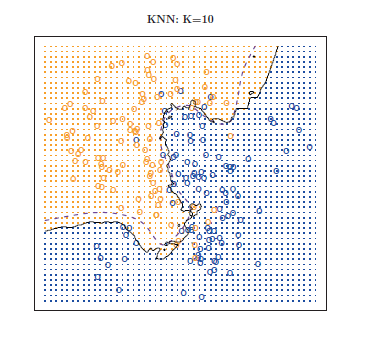
\includegraphics[width=0.6\textwidth]{knn1.png}}%
	\caption{Klasyfikacja dwuklasowa punktów na płaszczyźnie za pomocą algorytmu $k$-NN dla $k=10$. Czarną linią zaznaczono granicę decyzyjną klasyfikatora $k$-NN. Niebieską przerywaną linią zaznaczono granicę decyzyjną klasyfikatora Bayesa \cite{islr}}
\end{figure}

\begin{figure}[H]
	\centering
	\makebox[\textwidth][c]{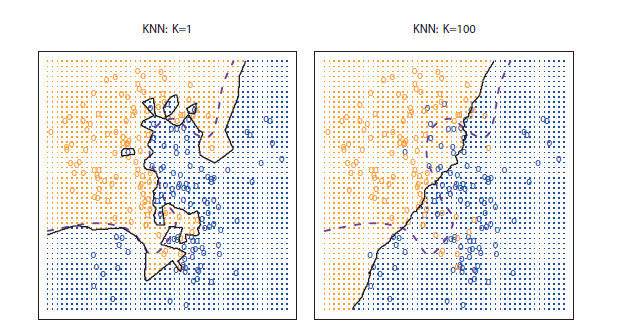
\includegraphics[width=1\textwidth]{knn2.png}}%
	\caption{Klasyfikacja dwuklasowa punktów na płaszczyźnie za pomocą algorytmu $k$-NN dla $k=1$ (lewa strona) i $k=100$ (prawa strona). Czarnymi liniami zaznaczono granicę decyzyjne klasyfikatorów $k$-NN. Niebieskimi przerywanymi liniami zaznaczono granice decyzyje klasyfikatorów Bayesa \cite{islr}}
\end{figure}

Na rysunku 4.4 przedstawiono wykresy błędu treningowego (niebieska linia) oraz testowego (żółta linia) w zależności od odwróconej wartości parametru $k$.  W roli danych testowych użyto 5000 obserwacji wygenerowanych z takiego samego rozkładu prawdopodobieństwa, co dane uczące. Kształty krzywych są podobne do kształtów zaprezentowanych wcześniej na rysunku 4.1. Z wykresu wynika, że w tym przypadku optymalna złożoność modelu jest osiągnięta dla $k \approx 10$. Można zauważyć, że wraz ze wzrostem wartości $k$ maleje wariancja modelu i rośnie jego obciążenie - odwrotnie niż zaprezentowano w poprzednim podrozdziale dla regresji wielomianowej. Pokazuje to, że intepretacja złożoności modelu jako liczby parametrów nie zawsze jest słuszna.

Równanie (4.6), opisujące kompromis między obciążeniem i wariancją, dla regresji metodą $k$-NN przyjmuje postać równiania (4.13) \cite{eslii}.
\begin{equation}
E(Y-\hat{Y})^2 = \sigma^2 + \big[f(X) - \frac{1}{k}\sum_{i=1}^{k}f(x_i)\big]^2 + \frac{\sigma^2}{k}
\end{equation}
$X$ oznacza obserwacje podaną na wejście klasyfikatora, $x_i$ oznacza $i$-tą  obserwację treningową. Składniki po prawej stronie równania to odpowiednio: błąd nieredukowalny $\sigma^2$ (jest to jednocześnie wariancja procesu generującego dane), obciążenie podniesone do kwadratu $\big[f(X) - \frac{1}{k}\sum_{i=1}^{k}f(x_i)\big]^2$ oraz wariancja modelu $\frac{\sigma^2}{k}$. Jak widać, wraz ze wzrostem wartości parametru $k$ rośnie obciążenie modelu i jednocześnie maleje wariancja. W związku z tym na wykresie z rysunku 4.4 wartość parametru $k$ odwrócono, aby wariancja modelu rosła wraz ze wzrostem wartości na osi odciętych.

\begin{figure}[H]
	\centering
	\makebox[\textwidth][c]{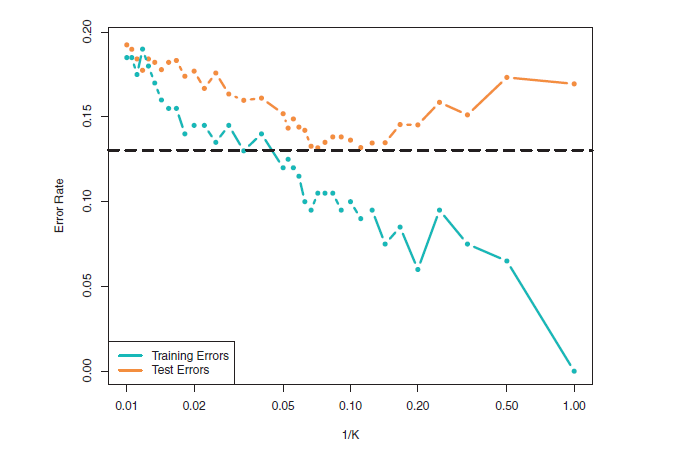
\includegraphics[width=1.05\textwidth]{knnerr.png}}%
	\caption{Wykres błędu treningowego (niebieska krzywa) i błędu testowego (żółta krzywa) klasyfikatora $k$-NN zależności od odwróconej wartości $k$. Dane treningowe zaprezentowano na rysunkach 4.2 i 4.3. Dane testowe (5000 obserwacji) nie zostały wykreślone. Zarówno dane treningowe jak i testowe zostały wygenerowane przez ten sam proces \cite{islr}}
\end{figure}

Stosowalność metody $k$-NN w przestrzeniach wysokowymiarowych jest ograniczona ze względu na zespół zjawisk zwany przekleństwem wymiarowości (ang. \textit{curse of dimensionality}). Termin ten został po raz pierwszy użyty przez Roberta Bellmana w odniesieniu do optymalizacji w przestrzeniach wysokowymiarowych \cite{bellman}. Współczenie terminu tego używa się do kilku różnych zjawisk wynikających z własności przestrzeni wysokowymiarowych.

W podrozdziale 4.1 zostało wspomniane, że jeżeli opracowany model statystyczny nie radzi sobie z poprawną klasyfikacją obserwacji testowych, to może to wynikać z zastosowania niedostatecznie licznego zbioru obserwacji treningowych. Zjawisko "przekleństwa" wymiarowości polega między innymi na tym, że liczba obserwacji potrzebna do skutecznego wytrenowania modelu rośnie wykładniczo wraz z wymiarowością \cite{islr} \cite{eslii}.

Na rysunku 4.5 pokazano pewien zbiór obserwacji w przestrzeniach: 1,2- oraz 3-wymiarowej. Wartości każdej ze zmiennych niezależnych znajdują się w przedziale $[0,20]$. Przedział ten jest dzielony na cztery równe podprzedziały: $[0,5)$, $[5,10)$, $[10,15)$, $[15,20]$. Przestrzeń można wtedy podzielić na $4^d$ regionów, gdzie $d$ oznacza wymiarowość przestrzeni. Jeżeli założy się, że w zbiorze obserwacji treningowych na każdy region powinno przypadać przynajmniej $p$ obserwacji, to całkowita liczba potrzebnych obserwacji treningowych rośnie wykładniczo. Na rysunku 4.5 liczba obserwacji pozostaje stała niezależnie od wymiarowości przestrzeni. W takim wypadku zwiększanie wymiarowości powoduje, że przestrzeń ta robi się coraz bardziej pusta (zjawisko pustej przestrzeni, ang. \textit{empty space phenomenon}, zostało pokazane na rysunku 4.5). 

\begin{figure}[H]
	\centering
	\makebox[\textwidth][c]{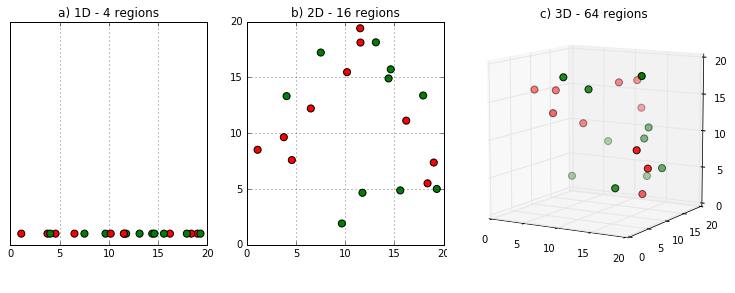
\includegraphics[width=1\textwidth]{curse.png}}%
	\caption{Zjawisko pustej przestrzeni. Zbiór obserwacji zrzutowano do przestrzeni 1-wymiarowej (lewa strona), 2-wymiarowej (środek) i 3-wymiarowej (prawa strona). Każdy z wymiarów podzielono na 4 przedziały. Wraz ze wzrostem liczby wymiarów wzrasta również liczba regionów przestrzeni, w których nie ma żadnych obserwacji \cite{curseimg}}
\end{figure}

"Przekleństwo" wymiarowości objawia się również na inne sposoby. W przypadku, gdy wartości predyktorów w poszczególnych wymiarach są niezależne i mają ten sam rozkład prawdopodobieństwa, to wraz ze wzrostem wymiarowości $d$ stosunek odległości do najdalszego sąsiada $D_{max}(d)$ i odległości do najbliższego  sąsiada $D_{min}(d)$ dąży do 1. Gdy wszystkie obserwacje są równo oddalone, pojęcie najbliższego sąsiada traci sens \cite{beyer}.

\begin{equation}
\lim\limits_{d\rightarrow+\infty} \frac{D_{max}(d)}{D_{min}(d)} = 1
\end{equation}






\section{Sieci neuronowe}
Sieci neuronowe są to struktury obliczeniowe wzorowane na budowie mózgu organizmów żywych. Mogą one zostać wykorzystane zarówno w zadaniach regresji, jak i klasyfikacji. Choć wiadomo, że sieci neuronowe nie są pełnym odwzorowaniem ludzkiego mózgu, to niemniej jednak znalazły one szerokie zastosowanie w m.in. przetwarzaniu i rozpoznawaniu obrazów czy dźwięku \cite{szegedy} \cite{purwins}.

Sieci neuronowe zbudowane są z podstawowych jednostek zwanych neuronami. Pojedynczy neuron posiada:
\begin{itemize}
	\item $n$ wejść, najczęściej oznaczanych $\mathbf{x} = [x_{1}, ... ,x_{n}]$,
	\item składową stała (ang. \textit{bias}) oznaczaną jako $b$,
	\item wagi, oznaczane $\mathbf{w} = [w_{1}, ..., w_{n}]$ - po jednej wadze na każde wejście,
	\item sumator,
	\item nieliniową funkcję aktywacji $f(\mathbf{x})$ oraz
	\item pojedyncze wyjście $y$.
\end{itemize}
Pojedynczy neuron realizuje równanie:
\begin{equation}
y = f(\mathbf{wx} + b)
\end{equation}

Neurony są uporządkowane w warstwy. Najprostsza sieć neuronowa posiada trzy warstwy: warstwę wejściową, warstwę ukrytą (pośrednią) oraz warstwę wyjściową. Wyjścia neuronów warstwy wejściowej są podawane na wejścia neuronów warstwy ukrytej, a wyjścia neuronów warstwy ukrytej - na wejścia neuronów warstwy wyjściowej. Tak zbudowana sieć neuronowa nazywana jest niekiedy perceptronem wielowarstwowym (ang. \textit{multilayer perceptron}). Możliwe jest zastosowanie dowolnej liczby warstw ukrytych. Liczba neuronów w każdej warstwie oraz schemat ich połączeń dobierany jest \textit{a priori}. Pomiędzy kolejnymi warstwami mogą być stosowane zarówno połączenia gęste  (ang. \textit{fully connected layers}), jak i połączenia rzadkie (ang. \textit{sparsely connected layers}). W warstwach gęsto połączonych każdy neuron warstwy wcześniejszej jest połączony ze wszystkimi neuronami warstwy późniejszej. Jeżeli tylko niektóre neurony kolejnych warstw są ze sobą połączone, to takie połączenia nazywamy rzadkimi \cite{haykin} \cite{sze}.

Poprzez odpowiednie dobranie wartości wag sieć neuronowa jest w stanie zaaproksymować dowolną funkcję $n$ zmiennych (gdzie $n$ jest liczbą wejść w warstwie wejściowej), pod warunkiem posiadania odpowiednio dużej liczby neuronów oraz warstw ukrytych. Jest to możliwe ze względu na zastosowanie nieliniowej funkcji aktywacji w każdym neuronie. Gdyby jej nie było, pojedynczy neuron byłby w stanie realizować tylko funkcje będące liniową kombinacją jego wejść \cite{cybenko} \cite{hornik}. Rolą składowej stałej jest przesuwanie funkcji aktywacji wzdłuż osi odciętych (osi wartości wejściowych) \cite{haykin}.

Tradycyjnie stosowaną funkcją aktywacji neuronu jest funkcja sigmoidalna \cite{haykin}:
\begin{equation}
\phi(x) = \frac{1}{1+e^{-x}}
\end{equation}
Sigmoidalna funkcja aktywacji bywa problematyczna ze względu na problem zanikającego gradientu (ang. \textit{vanishing gradient problem}) - dla pobudzeń mocno oddalonych od $0$ wartość gradientu jest bardzo niska, co utrudnia bądź uniemożliwia uczenie \cite{bengio} \cite{hochreiter}. Zjawisko to jest szczególnie uciążliwe w sieciach neuronowych z dużą liczbą warstw ukrytych. Z tego też powodu często jest stosowana tzw. funkcja ReLU (ang. \textit{Rectified Linear Unit}). Jest ona dana wzorem \cite{glorot}:
\begin{equation}
ReLU(x) = max(0,x)
\end{equation}
Zastosowanie funkcji ReLU częściowo rozwiązuje problem zanikającego gradientu. Ponadto, stosowanie funkcji ReLU często skutkuje wyższą dokładnością w zadaniach klasyfikacji oraz mniejszą liczbą epok uczenia potrzebną do osiągnięcia pożądanego rezultatu \cite{jarrett} \cite{glorot} \cite{nair}. Dodatkową zaletą funkcji ReLU jest niewielki koszt obliczeniowy. Funkcja ReLU jest powszechnie używaną domyślną funkcją aktywacji w warstwach ukrytych. Modyfikacją funkcji ReLU jest tzw. ''nieszczelna'' funkcja ReLU (ang. \textit{Leaky ReLU}), umożliwiająca przepływ gradientu w przypadku ujemnych pobudzeń:

\begin{equation}
LReLU(x) = \begin{cases}
x & x \geq 0 \\
ax, & x < 0
\end{cases} \qquad 0 < a < 1
\end{equation}
Parametr nachylenia $a$ dobierany jest \textit{a priori}. Często spotykaną wartością jest $a = 0.01$ \cite{goodfellow}.

Szczególną funkcją aktywacji jest funkcja \textit{softmax}. Dla $i$-tej wartości wektora wyjściowego jest ona zdefiniowana następująco \cite{goodfellow}:
\begin{equation}
softmax(x_{i}) = \frac{e^{x_i}}{\sum_{j = 1}^{n}e^{x_j}}
\end{equation}
Funkcja \textit{softmax} posiada dwie interesujące własności:
\begin{itemize}
	\item każdy z elemenów wektora odpowiedzi przyjmuje wartość z przedziału $[0;1]$,
	\item suma wartości wektora odpowiedzi jest zawsze równa 1.
\end{itemize}
Jest ona stosowana w warstwie wyjściowej sieci w zadaniach klasyfikacji $n$-klasowej, gdzie $n$ oznacza liczbe neuronów warstwy wyjściowej. Wtedy $i$-tą wartość wektora odpowiedzi można interpretować jako prawdopodobieństwo przynależności podanej obserwacji do $i$-tej klasy \cite{goodfellow} \cite{nwakpa}. Wyjątkiem jest klasyfikacja 2-klasowa - w takiej sytuacji w warstwie wyjściowej typowo używa się pojedynczego neuronu z sigmoidalną funkcją aktywacji.

W zadaniach regresji najczęściej używaną funkcją błędu jest błąd średniokwadratowy dany równaniem (4.1). W zadaniach klasyfikacji powszechnie używaną funkcją błędu jest tzw. funkcja \textit{cross-entropy}:
\begin{equation}
CE = \frac{1}{N}\sum_{i=1}^{N}y_i\text{log}(\hat{y}_i)
\end{equation}
$N$ oznacza liczbę obserwacji treningowych, $y_i$ oznacza zmienną zależna $i$-tej obserwacji treningowej, natomiast $\hat{y}_i$ oznacza wartość (klasę) zwróconą przez sieć neuronową w odpowiedzi na $i$-tą obserwacje treningową.

Uczenie sieci neuronowych polega na znalezieniu takiego zestawu wag sieci $\mathbf{w}$ i obciążeń $\mathbf{b}$, dla których wartość funkcji błędu dla zadanego zbioru danych treningowych jest możliwie najmniejsza. Minimalizacja funkcji błędu najczęściej odbywa się poprzez metody gradientowe (ang. \textit{gradient descent}) \cite{goodfellow}. 

Metoda gradientu prostego jest iteracyjną metodą znajdowania minimum funkcji. Polega ona na obliczeniu gradientu funkcji błędu $\nabla J(\mathbf{w},\mathbf{b})$ dla pewnego argumentu $(\mathbf{w}_0,\mathbf{b}_0)$, nazywanego punktem startowym, i wykonaniu kroku w kierunku przeciwnym do kierunku gradientu. Długość kroku określona jest przez długość wektora gradientu $|\nabla J(\mathbf{w},\mathbf{b})|$ oraz współczynnik kroku $\eta$. Współczynnik kroku w literaturze dotyczącej sieci neuronowych określany jest również jako tempo uczenia (ang. \textit{learning rate)} \cite{ruder}:
\begin{equation}
\begin{split}
\mathbf{w}_{i+1} = \mathbf{w}_i - \eta\nabla J(\mathbf{w}) \\
\mathbf{b}_{i+1} = \mathbf{b}_i - \eta\nabla J(\mathbf{b})
\end{split}
\end{equation}
Kierunek gradientu określa kierunek najszybszego wzrostu wartości funkcji. Wykonanie kroku w kierunku przeciwnym spowoduje spadek wartości funkcji, jeżeli wykonany krok jest wystarczająco mały. Algorytm kończy działanie, gdy wykonywanie kolejnych kroków nie powoduje dalszego spadku wartości funkcji. Metodę gradientową można zastosować tylko do optymalizacji funkcji ciągłych i różniczkowalnych. Z tego też powodu funkcja błędu klasyfikacji, dana równaniem (4.2) nie jest używana w procesie uczenia sieci neuronowych.

W standardowej metodzie gradientu w każdej iteracji wykorzystywane są wszystkie obserwacje treningowe. Takie podejście jest niepraktyczne ze względu na fakt, że do treningu sieci neuronowych często korzysta się z bardzo dużych zbiorów danych. Możliwym rozwiązaniem jest zastosowanie stochastycznej metody gradientu (ang. \textit{stochastic gradient descent}) - wtedy w każdej iteracji wykorzystywany jest tylko jedna obserwacja pomiarowa. Umożliwia to bardziej częste aktualizacje wag sieci, a także uczenie sieci w trakcie jej działania (ang. \textit{online training}). Częstym skutkiem ubocznym takiego podejścia są duże fluktuacje wartości funkcji celu w trakcie uczenia. Kompromisem między tymi dwoma podejściami jest stosowanie porcji danych treningowych (ang. \textit{mini-batch}) w każdej iteracji. Typowy rozmiar porcji to 50-256 obserwacji. Porcjowanie danych treningowych jest obecnie standardowym podejściem \cite{goodfellow} \cite{ruder}. 

Metoda gradientu nie gwarantuje znalezienia globalnego minimum funkcji. 
Kluczowe znaczenie ma wartość parametru $\eta$. Gdy jest ona zbyt mała, to po wpadnięciu w lokalne minimum algorytm nie będzie w stanie się z niego wydostać. Zbyt wysoka wartość $\eta$ spowoduje, że algorytm może nie osiągnąć nawet lokalnego minimum, gdyż będzie ''przeskakiwać'' ponad nim ze względu na wykonywanie zbyt dużych kroków. Najprostszym obejściem tego problemu jest zastosowanie wysokiej wartości $\eta$ i zmniejszanie jej w każdej iteracji. W ten sposób w pierwszych iteracjach metoda wykonuje duże kroki, potencjalnie przenosząc się w okolice globalnego minimum, a w dalszych iteracjach wykonywać małe kroki \cite{ruder}. 

Współcześnie do treningu sieci neuronowych często używane są zmodyfikowane warianty metody gradientu, w których każdej wadze sieci przyporządkowany jest oddzielny współczynnik kroku. Wartości wszystkich współczynników kroku są w każdej iteracji adaptacyjnie modyfikowane. Przykładami takich metod optymalizacji są m.in. \textit{AdaGrad}, \textit{RMSProp} czy \textit{Adam} \cite{duchi} \cite{kingma} \cite{ruder}.

Do obliczania wartości gradientów w sieci neuronowej używana jest metoda zwana propagacją wsteczną (ang. \textit{backpropagation}) \cite{rumelhart}. Propagacja wsteczna polega na regule łancuchowej obliczania pochodnych funkcji złożonych. Niech $g:\mathbb{R}^m \rightarrow \mathbb{R}^n$, $f:\mathbb{R}^n \rightarrow \mathbb{R}$, $\mathbf{y}=g(\mathbf{x})$, $z=f(\mathbf{y})$. Wtedy zgodnie z regułą łańuchową \cite{goodfellow}:

\begin{equation}
\frac{\partial z}{\partial x_i} = \sum_{j}^{}\frac{\partial z}{\partial y_j}\frac{\partial y_j}{\partial x_i}
\end{equation}

Metoda propagacji wstecznej została zaprezentowana na przykładzie prostej sieci neuronowej pokazanej na rysunku 4.6. Sieć ta złożona jest z sześciu neuronów $n_{1...6}$ uporządkowanych w trzy warstwy: wejściową, ukrytą oraz wyjściową. Każdy neuron posiada sigmoidalną funkcję aktywacji:
\begin{equation}
\phi(z) = \frac{1}{1 + e^{-z}}
\end{equation}
Pochodna funkcji sigmoidalnej względem wejścia przyjmuje postać \cite{minai}:
\begin{equation}
\frac{d\phi(z)}{dz} = \phi(z)(1 - \phi(z))
\end{equation}
Niech $w_{i,j}$ oznacza wagę połączenia pomiędzy neuronami $n_i$ oraz $n_j$. Niech $b_i$ oznacza składową stałą podawaną na wejście neuronu $n_i$. Niech $net_i$ oznacza ważoną sumę wejść neuronu $n_i$, a $out_i$ - wyjście neuronu $n_i$:
\begin{equation}
out_i = \phi(net_i) = \phi\left(\sum_{j}^{}w_{j,i}out_j\right)
\end{equation}
Niech $\mathbf{x} = [x_1, x_2]$ oznacza obserwację treningową podaną na wejście sieci neuronowej. Niech $\mathbf{y} = [y_1, y_2]$ oznacza pożądaną odpowiedź sieci neuronowej na $\mathbf{x}$. Niech $\mathbf{out} = [out_5, out_6]$ oznacza faktyczną odpowiedź sieci neuronowej na $\mathbf{x}$. 
Niech $E_{n_5}$ i $E_{n_6}$ będą przeskalowanymi wartościami funkcji błędu średniokwadratowego pomiędzy odpowiednio $out_5$ i $y_1$ oraz $out_6$ i $y_2$. Niech $E_{total}$ będzie całkowitą wartością przeskalowanej funkcji błędu średniokwadratowego \cite{rojas}:
\begin{equation}
E_{total} = \frac{1}{2}||\mathbf{out} - \mathbf{y}||^2 = \frac{1}{2}(out_{n_5} - y_1)^2 + \frac{1}{2}(out_{n_6} - y_2)^2
\end{equation}
\begin{equation}
E_{n_5} = \frac{1}{2}(out_{n_5} - y_1)^2
\end{equation}
\begin{equation}
E_{n_6} = \frac{1}{2}(out_{n_6} - y_2)^2
\end{equation}

\begin{figure}[H]
	\centering
	\makebox[\textwidth][c]{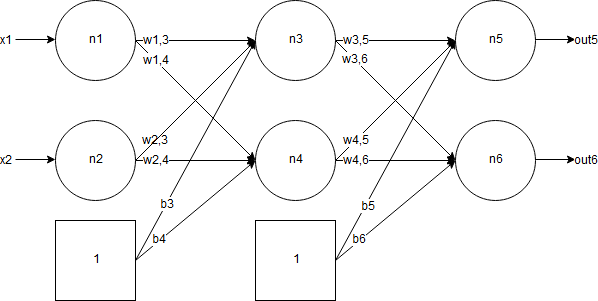
\includegraphics[width=1\textwidth]{nn2.png}}%
	\caption{Przykładowa sieć neuronowa przedstawiona w postaci grafu.}
\end{figure}

Pierwszym etapem propagacji wstecznej jest tzw. \textit{forward pass}. Najpierw na wejście sieci podawana jest obserwacja treningowa $\mathbf{x}$. Każdy neuron $n_i$ zapamiętuje ważoną sumę swoich wejść $net_i$. Na jej podstawie wyliczana jest wartość wyjściowa neuronu $out_i$. Operacja ta jest powtarzana w każdej warstwie aż do obliczenia wartości wyjściowych neuronów w ostatniej warstwie $out_{n_5}$, $out_{n_6}$. Na podstawie tych wartości wyjściowych oraz wartości pożądanych $y_1$, $y_2$ obliczane są wartości funkcji błędu $E_{n_5}$, $E_{n_6}$ dla każdego neuronu w warstwie wyjściowej. Ostatecznie obliczana jest łączna wartość funkcji błędu $E_{total}$.

Drugim, właściwym etapem propagacji wstecznej jest \textit{backward pass}. W tej fazie w każdej warstwie począwszy od warstwy wyjściowej obliczane są pochodne cząstkowe funkcji błędu $E_{total}$ poprzez zastosowanie reguły łańcuchowej. Przykładowo, pochodna $E_{total}$ względem wagi $w_{3,5}$ obliczana jest w następujący sposób:

\begin{equation}
\frac{\partial E_{total}}{\partial w_{3,5}} = \frac{\partial E_{total}}{\partial out_{n_5}}\frac{\partial out_{n_5}}{\partial net_{n_5}}\frac{\partial net_{n_5}}{\partial w_{3,5}}
\end{equation}

Pochodna funkcji całkowitego błędu $E_{total}$ względem wyjścia $out_{n_5}$ przyjmuje postać:

\begin{equation}
\begin{split}
\frac{\partial E_{total}}{\partial out_{n_5}} & = \frac{\partial E_{n_5}}{\partial out_{n_5}} + \frac{\partial E_{n_6}}{\partial out_{n_5}} = \\ & = \frac{\partial \frac{1}{2}(out_{n_5} - y_1)^2}{\partial out_{n_5}} + \frac{\partial \frac{1}{2}(out_{n_6} - y_2)^2}{\partial out_{n_5}} = \\ & = out_{n_5} - y_1
\end{split}
\end{equation}
Pochodna wyjścia $out_{n_5}$ względem wejścia $net_{n_5}$ przyjmuje postać:

\begin{equation}
\frac{\partial out_{n_5}}{\partial net_{n_5}} = \frac{\partial \phi(net_{n_5})}{\partial net_{n_5}} = \phi (net_{n_5})(1 - \phi(net_{n_5}))
\end{equation}
Pochodna wejścia $net_{n_5}$ względem wagi $w_{3,5}$ przyjmuje postać:

\begin{equation}
\frac{\partial net_{n_5}}{\partial w_{3,5}} = \frac{\partial (out_{n_3}w_{3,5} + out_{n_4}w_{4,5} + b_5)}{\partial w_{3,5}} = out_{n_3}
\end{equation}
Wyrażenie z równania (4.29) przyjmuje ostateczną postać:

\begin{equation}
\frac{\partial E_{total}}{\partial w_{3,5}} = (out_{n_5} - y_1)\phi(net_{n_5})(1 - \phi(net_{n_5}))out_{n_3}
\end{equation}
Pochodna funkcji całkowitego błędu $E_{total}$ względem wag $w_{3,6}, w_{4,5}, w_{4,6}$ oraz obciążeń $b_5,b_6$ obliczana jest analogicznie. 

Nieco inny jest sposób obliczania pochodnej funkcji całkowitego błędu $E_{total}$ względem wag w warstwie ukrytej. Przykładowo, pochodna po $E_{total}$ względem wagi $w_{1,3}$ przyjmuje postać:

\begin{equation}
\frac{\partial E_{total}}{\partial w_{1,3}} = \frac{\partial E_{total}}{\partial out_{n_3}}\frac{\partial out_{n_3}}{\partial net_{n_3}}\frac{\partial net_{n_3}}{\partial w_{1,3}}
\end{equation}
Pierwszy czynnik wyrażenia po prawej stronie równania (4.34) obliczany jest następująco
\begin{equation}
\frac{\partial E_{total}}{\partial out_{n_3}} = \frac{\partial E_{n_5}}{\partial out_{n_3}} + \frac{\partial E_{n_6}}{\partial out_{n_3}} 
\end{equation}
\begin{equation}
\begin{split}
\frac{\partial E_{n_5}}{\partial out_{n_3}} & = \frac{\partial E_{n_5}}{\partial out_{n_5}}\frac{\partial out_{n_5}}{\partial net_{n_5}}\frac{\partial net_{n_5}}{\partial out_{n_3}} = \\ & =
(out_{n_3} - y_1)\phi(net_{n_5})(1 - \phi(net_{n_5}))w_{3,5}
\end{split}
\end{equation}
\begin{equation}
\begin{split}
\frac{\partial E_{n_6}}{\partial out_{n_3}} & = \frac{\partial E_{n_6}}{\partial out_{n_6}}\frac{\partial out_{n_6}}{\partial net_{n_6}}\frac{\partial net_{n_6}}{\partial out_{n_3}} = \\ & =
(out_{n_3} - y_2)\phi(net_{n_6})(1 - \phi(net_{n_6}))w_{3,6}
\end{split}
\end{equation}

\begin{equation}
\begin{split}
\frac{\partial E_{total}}{\partial out_{n_3}}  = & (out_{n_3} - y_1)\phi(net_{n_5})(1 - \phi(net_{n_5}))w_{3,5} + \\ & (out_{n_3} - y_2)\phi(net_{n_6})(1 - \phi(net_{n_6}))w_{3,6}
\end{split}
\end{equation}
Drugi czynnik wyrażenia po prawej stronie równania (4.34) obliczany jest jak w równaniu (4.31):

\begin{equation}
\frac{\partial out_{n_3}}{\partial net_{n_3}} = \frac{\partial \phi(net_{n_3})}{\partial net_{n_3}} = \phi (net_{n_3})(1 - \phi(net_{n_3}))
\end{equation}
Ostatni czynnik obliczany jest w następujący sposób:

\begin{equation}
\frac{\partial net_{n_3}}{\partial w_{1,3}} = \frac{\partial (out_{n_1}w_{1,3} + out_{n_2}w_{2,3} + b_3)}{\partial w_{1,3}} = out_{n_1}
\end{equation}
Pochodne $E_{total}$ względem pozostałych wag i obciążeń w dalszych warstwach obliczane są w analogiczny sposób.

Przebieg procesu treningu sieci neuronowej jest silnie uzależniony od wyboru punktu startowego. Dobór początkowego zestawu parametrów sieci wpływa na tempo zbieżności algorytmu optymalizacyjnego, uwarunkowanie numeryczne zadania, a także na błąd generalizacji. Problematyka inicjalizacji wag sieci neuronowej nie jest obecnie dobrze zrozumiana. Z tego też powodu powszechnie stosowane metody inicjalizacji wag sieci neuronowych są metodami heurystycznymi \cite{goodfellow}.

Popularną metodą inicjalizacji wag sieci neuronowych jest metoda zaproponowana przez Glorot i Bengio \cite{glorot2}. W metodzie tej wartość wagi $w_i$ jest losowana z następującego rozkładu:

\begin{equation}
w_i \sim U\left[ -\frac{1}{\sqrt{n}}, \frac{1}{\sqrt{n}}\right]
\end{equation}
$U[-a,a]$ oznacza rozkład równomierny na przedziale $(-a,a)$, natomiast $n$ oznacza liczbe neuronów w warstwie poprzedniej. Składowe stałe $\textbf{b}$ są inicjalizowane wartością zerową.

Popularną modyfikacją metody Glorot i Bengio, przystosowaną do funkcji aktywacji z rodziny ReLU, jest metoda inicjalizacji zaproponowana przez He i in. \cite{he}:
\begin{equation}
w_i \sim U\left[ -\frac{2}{\sqrt{n}}, \frac{2}{\sqrt{n}}\right]
\end{equation}

Ważnym elementem treningu sieci neuronowej jest regularyzacja. Regularyzacja to zbiór technik mających na celu poprawę zdolności generalizacji sieci \cite{goodfellow}. Inaczej mówiąc, regularyzacja ma na celu zmniejszenie błędu testowego modelu bez wpływu na błąd treningowy. Poniżej opisane zostaną niektóre z powszechnie stosowanych technik regularyzacji.

Podczas uczenia sieci neuronowych zdarza się, że błąd walidacji zaczyna rosnąć pomimo tego, że błąd treningowy ciągle maleje. Oznacza to, że można opracować model z lepszymi zdolnościami regularyzacji, powracając do zestawu parametrów, dla którego błąd walidacji był minimalny. Technika ta nosi nazwę \textit{early stopping}. Stosując \textit{early stopping} należy wcześniej ustalić wartość parametru zwanego cierpliwością (ang. \textit{patience}). Cierpliwość określa maksymalną liczbę epok uczenia w trakcie której model powinien osiągnąć nowe minimum błędu walidacji. Jeżeli nowe minimum nie zostanie osiągnięte w wyznaczonej liczbie epok, proces uczenia jest przerywany, a wagi sieci zostają przywrócone do wartości zapewniających osiągnięte minimum. \textit{Early stopping} polepsza zdolności generalizacji sieci poprzez przeciwdziałanie nadmiernemu dopasowaniu do danych (\textit{overfitting}) \cite{goodfellow}.  

Inną popularną metodą regularyzacji jest dodanie do funkcji błędu składnika ''kary'' zależnego od wartości wag sieci \cite{goodfellow}. Wpływ składnika kary determinowany jest przez dobrany \textit{a priori} parametr kary $\lambda$.
\begin{equation}
\tilde{J}(\mathbf{w},\mathbf{b}) = J(\mathbf{w},\mathbf{b}) + \lambda\Omega(\mathbf{w})
\end{equation}
Powoduje to, że w trakcie uczenia preferowane jest dobieranie wagom niższych wartości. Technika ta nazywana jest \textit{weight decay}. Najpopularniejsza  funkcja kary to kara w normie $L^2$ zwana również regularyzacją Tichonowa:
\begin{equation}
\Omega_{L^2}(\mathbf{w}) = \frac{1}{2}\sum_{i}^{}w_{i}^{2} = \frac{1}{2}\mathbf{w}^{T}\mathbf{w}
\end{equation}
Inna możliwa funkcja kary to kara w normie $L^1$:
\begin{equation}
\Omega_{L^1}(\mathbf{w}) = \frac{1}{2}\sum_{i}^{}|w_{i}|
\end{equation}
Należy zaznaczyć, że składnik kary nie obejmuje wartości składowych stałych.

\section{Maszyna wektorów nośnych}
Maszyna wektorów nośnych jest to metoda klasyfikacji będąca uogólnieniem klasyfikatora maksymalnego marginesu. Została ona opracowana przez Vapnika i Cortes \cite{cortes}. 

Obserwacje $(\mathbf{x}_1,y_1), ..., (\mathbf{x}_n,y_n)$ z przyporządkowanymi binarnymi klasami $y_i \in \{-1,1\}$ są liniowo separowalne, jeżeli istnieje hiperpłaszczyzna $H(\mathbf{x})$ postaci:
\begin{equation}
H(\mathbf{x}) = \mathbf{w}^T\mathbf{x} + b
\end{equation}
dla której zachodzi:
\begin{equation}
\begin{cases}
H(\mathbf{x}_i) > 0,\ y_i = 1, \\
H(\mathbf{x}_i) < 0,\ y_i = -1, \\
\end{cases}
\end{equation}

Spośród wszystich możliwych hiperpłaszczyzn separujących istnieje szczególna hiperpłaszczyzna zwana klasyfikatorem maksymalnego marginesu (ang. \textit{maximum margin classifier}), którego odległość od najbliższej obserwacji (zwana marginesem) jest możliwie największa. Szerszy margines zapewnia lepszą zdolność generalizacji klasyfikatora \cite{islr} \cite{eslii}. Na rysunku 4.7 po lewej stronie pokazano kilka możliwych hiperpłaszczyzn separujących obserwacje z przypisanymi binarnymi klasami (kolorami). Po prawej stronie rysunku 4.7 przedstawiono klasyfikator maksymalnego marginesu dla tej samej grupy punktów. 
\begin{figure}[H]
	\centering
	\makebox[\textwidth][c]{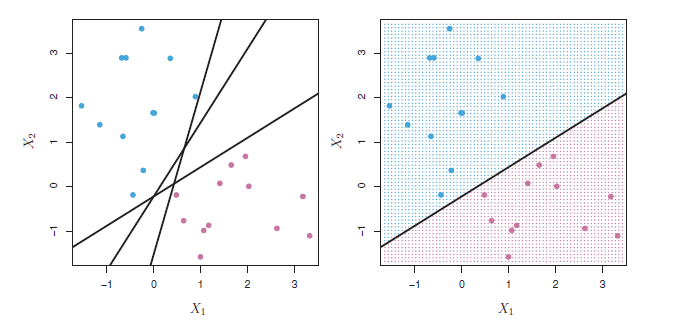
\includegraphics[width=1.1\textwidth]{margin1.png}}%
	\caption{Niebieskimi kropkami zaznaczono obserwacje przypisane do klasy $y = 1$, a fioletowymi kropkami obserwacje przypisane do klasy $y = -1$. Czarnymi liniami oznaczono przykładowe hiperpłaszczyzny separujące (lewa strona). Czarną linią oznaczono klasyfikator maksymalnego marginesu (prawa strona) \cite{islr}}
\end{figure}
Konstrukcja klasyfikatora maksymalnego marginesu sprowadza się do rozwiązania następującego problemu optymalizacyjnego \cite{islr} \cite{eslii}:
\begin{equation}
\begin{array}{lll}
\text{max}\ M &\\
\sum_{j=1}^{p} w_{j}^{2} = 1, &\\
y_i(\mathbf{w}^T\mathbf{x}_i + b) \ge M, & \forall i = 1,...,n
\end{array}
\end{equation}
gdzie $M$ oznacza szerokość marginesu, czyli odległość do najbliższej obserwacji, $n$ oznacza liczbę obserwacji, a $p$ ich wymiarowość.

Klasyfikator maksymalnego marginesu nie dopuszcza do niepoprawnego zaklasyfikowana żadnej z obserwacji treningowych. Z tego powodu jest bardzo wrażliwy na obserwacje odstające. Dodanie nawet jednej obserwacji odstającej może spowodować zmianę nachylenia hiperpłaszczyzny oraz zwężenie marginesu. Sytuacja taka jest pokazana na rysunku 4.8.
\begin{figure}[H]
	\centering
	\makebox[\textwidth][c]{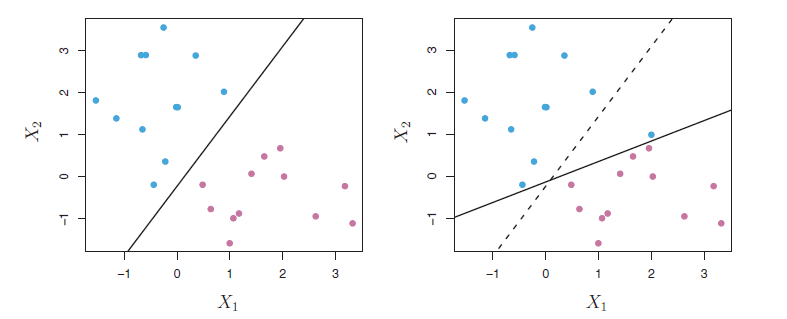
\includegraphics[width=1.1\textwidth]{margin2.png}}%
	\caption{Czarną linią przedstawiono klasyfikator maksymalnego marginesu dla pewnego zbioru danych (lewa strona). Po dodaniu dodatkowej obserwacji współczynniki klasyfikatora maksymalnego marginesu ulegają znacznej modyfikacji. Szerokość marginesu zostaje zmniejszona (prawa strona) \cite{islr}}
\end{figure}
Klasyfikator maksymalnego marginesu można ulepszyć dopuszczając niepoprawne zaklasyfikowanie niewielkiej liczby obserwacji treningowych. Ma to na celu zmniejszenie wrażliwości na obserwacje odstające. Taki klasyfikator nazywany jest klasyfikatorem miekkiego marginesu (ang. \textit{soft margin classifier}). Konstrukcja klasyfikatora miękkiego marginesu jest równoznaczna z rozwiązaniem następującego problemu optymalizacyjnego \cite{islr}:
\begin{equation}
\begin{array}{ll}
\text{max}\ M &\\
\sum_{j=1}^{p} w_{j}^{2} = 1, \\
y_i(\mathbf{w}^T\mathbf{x}_i + b) \ge M(1 - \epsilon_i), & \forall i = 1,...,n \\
\epsilon_i \ge 0, & \forall i = 1,...,n  \\
\sum_{i=1}^{n} \epsilon_i \le C\\ 
\end{array}
\end{equation}
Zmienne $\epsilon_{1...n}$ określają położenie $i$-tej obserwacji treningowej względem hiperpłaszczyzny i marginesów. Jeżeli $\epsilon_i = 0$, to $i$-ta obserwacja znajduje się po właściwej stronie marginesu. Jeżeli $\epsilon_i > 0$, to $i$-ta obserwacja znajduje się po niewłaściwej stronie marginesu, natomiast jeżeli $\epsilon_i > 1$, to  $i$-ta obserwacja znajduje się po niewłaściwej stronie hiperpłaszczyzny. Wartość parametru $C$ (dobierana \textit{a priori}) określa więc maksymalną dopuszczalną liczbę nieprawidłowo zaklasyfikowanych obserwacji treningowych. Wpływ wartości parametru $C$ na klasyfikator miekkiego marginesu przedstawiono na rysunku 4.9 \cite{islr}.
\begin{figure}[H]
	\centering
	\makebox[\textwidth][c]{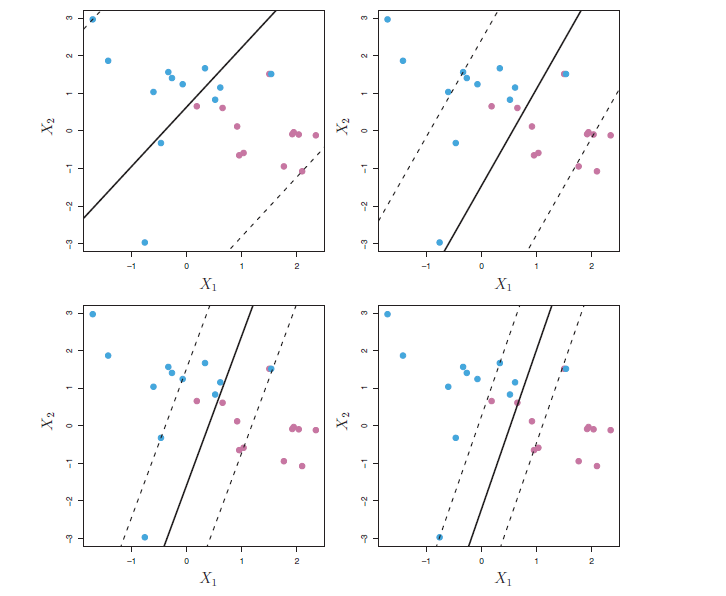
\includegraphics[width=1.1\textwidth]{margin3.png}}%
	\caption{Wpływ wartości parametru $C$ na klasyfikator miekkiego marginesu. Wykresy w kolejności od największej wartości $C$ do najmniejszej: lewy górny, prawy górny, lewy dolny, prawy dolny. Ciągłymi liniami zaznaczono granice klasyfikacji. Przerywanymi liniami zaznaczono marginesy \cite{islr}}
\end{figure}
Maszyna wektorów nośnych jest rozszerzeniem klasyfikatora miękkiego marginesu pozwalająca na dokładniejszą klasyfikację danych nieseparowalnych liniowo. W tej metodzie klasyfikacji obserwacje treningowe są odwzorowywane na przestrzeni o wyższej wymiarowości za pomocą pewnego przekształcenia $\phi(\mathbf{x})$. W tak otrzymanej przestrzeni obserwacje są separowalne liniowo (w idealnym przypadku) lub ich błąd klasyfikacji jest mniejszy niż w pierwotnej przestrzeni. Przykład takiego odwzorowania pokazano na rysunku 4.10.
\begin{figure}[H]
	\centering
	\makebox[\textwidth][c]{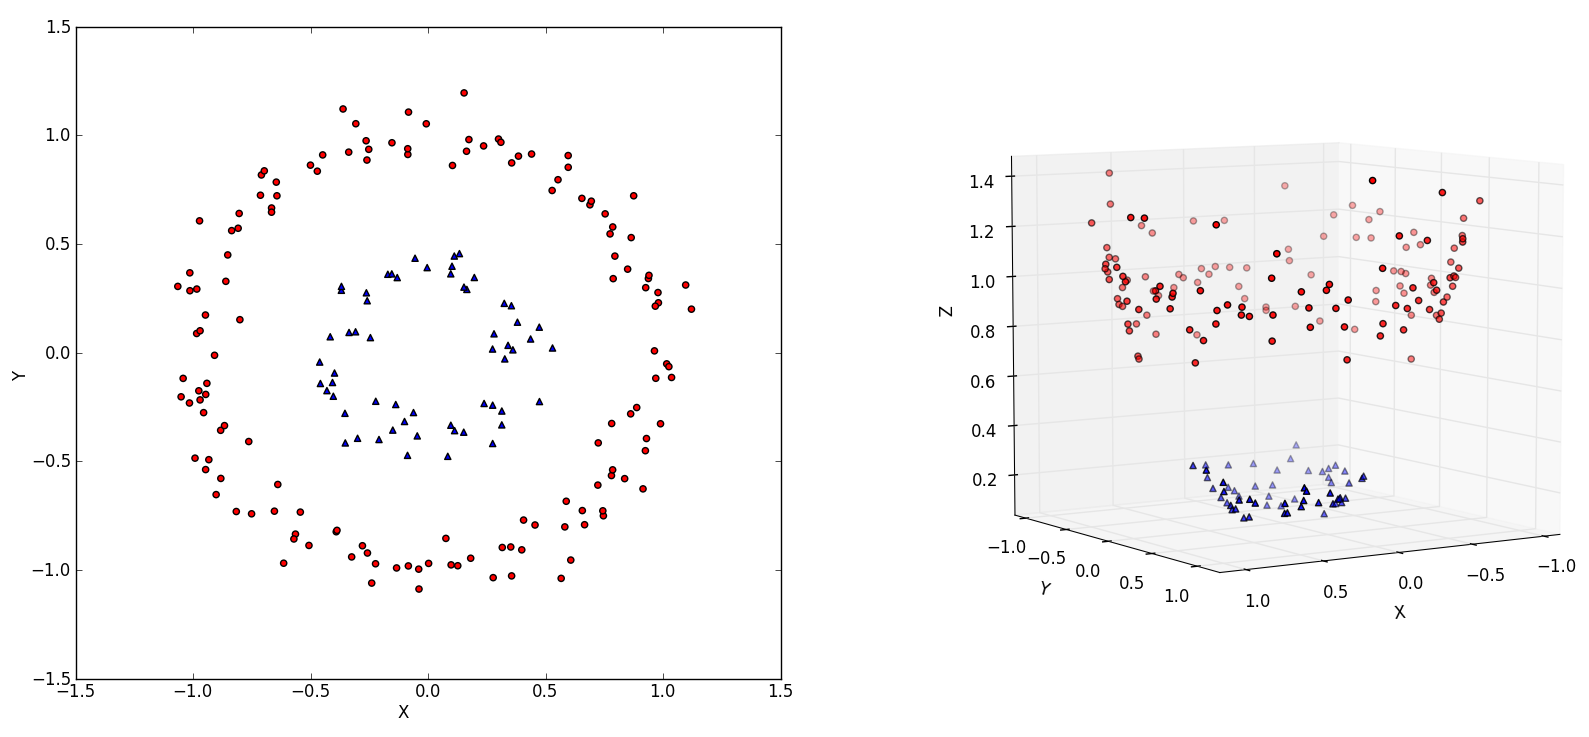
\includegraphics[width=1\textwidth]{svm1a.png}}%
	\caption{Dane w przestrzeni 2-wymiarowej są nieseparowalne liniowo (lewa strona). Dane po przeniesieniu do przestrzeni 3-wymiarowej za pomocą przekształcenia $\phi: [x,y] \rightarrow [x,y,x^2+y^2]$ stają się liniowo separowalne (prawa strona) \cite{svmimg}}
\end{figure}
\noindent Zrzutowanie wynikowej hiperpłaszczyzny separującej na pierwotną przestrzeń cech w efekcie daje nieliniową granicę decyzyjną, co pokazano na rysunku 4.11.

Wadą przedstawionego rozwiązania jest wielokrotne zwiększenie wymiarowości problemu, co może spowodować bardzo długi czas opracowywania modelu. Rozwiązywane jest to za pomocą metody zwanej \textit{kernel trick}. 
Problem konstrukcji maszyny wektorów nośnych z przekształceniem $\phi$ można przedstawić jako poniższy problem optymalizacyjny \cite{eslii}:
\begin{equation}
\begin{array}{ll}
\text{max}\ \sum_{i=1}^{n}\alpha_i - \frac{1}{2}\sum_{i=1}^{n}\sum_{j=1}^{n}\alpha_i\alpha_jy_iy_j\langle\phi(\mathbf{x}_i),\phi(\mathbf{x}_j)\rangle &\\
0 \le \alpha_i \le C, & \forall i = 1,...,n  \\
\sum_{i=1}^{n}\alpha_iy_i = 0, & \forall i = 1,...,n
\end{array}
\end{equation}
gdzie $\alpha_{1...n}$ to mnożniki Lagrange'a. Należy zaznaczyć, że w tak sformułowanym problemie duża wartość $C$ oznacza małą tolerancję na błędy klasyfikacji, przeciwnie niż na rysunku 4.9. 

Rozwiązaniem problemu jest funkcja opisana równaniem \cite{eslii}:
\begin{equation}
f(\mathbf{x}) = \sum_{i=1}^{n}\alpha_iy_i\langle\phi(\mathbf{x}),\phi(\mathbf{x}_i)\rangle + b
\end{equation}
Jak widać, zarówno optymalizowana funkcja, jak i równanie opisujące wynikową hiperpłaszczyznę nie korzystają bezpośrednio z przekształcenia $\phi(\mathbf{x})$, ale jedynie z wartości iloczynu skalarnego pary przekształconych obserwacji. Iloczyn skalarny w obydwu wyrażeniach można zastąpić pewną funkcją $K(\mathbf{x}_1,\mathbf{x}_2)$ zwaną funkcją rdzenia lub kernelem, która przyjmuje wartości równe wartościom iloczynu skalarnego przekształconych obserwacji $\mathbf{x}_1,\mathbf{x}_2$ bez obliczania wartości $\phi(\mathbf{x}_1),\phi(\mathbf{x}_2)$.
\begin{equation}
K(\mathbf{x}_1,\mathbf{x}_2) = \langle\phi(\mathbf{x}_1),\phi(\mathbf{x}_2)\rangle
\end{equation}
Do popularnych kerneli należą wielomiany $d$-tego stopnia oraz radialne funkcje bazowe (ang. \textit{radial basis function}, \textit{RBF}), dane wzorem:
\begin{equation}
RBF(\mathbf{x}_1,\mathbf{x}_2) = e^{-\gamma||\mathbf{x}_1-\mathbf{x}_2||^2}
\end{equation}
gdzie $\gamma > 0$ jest parametrem dobieranym \textit{a priori}.
\begin{figure}[H]
	\centering
	\makebox[\textwidth][c]{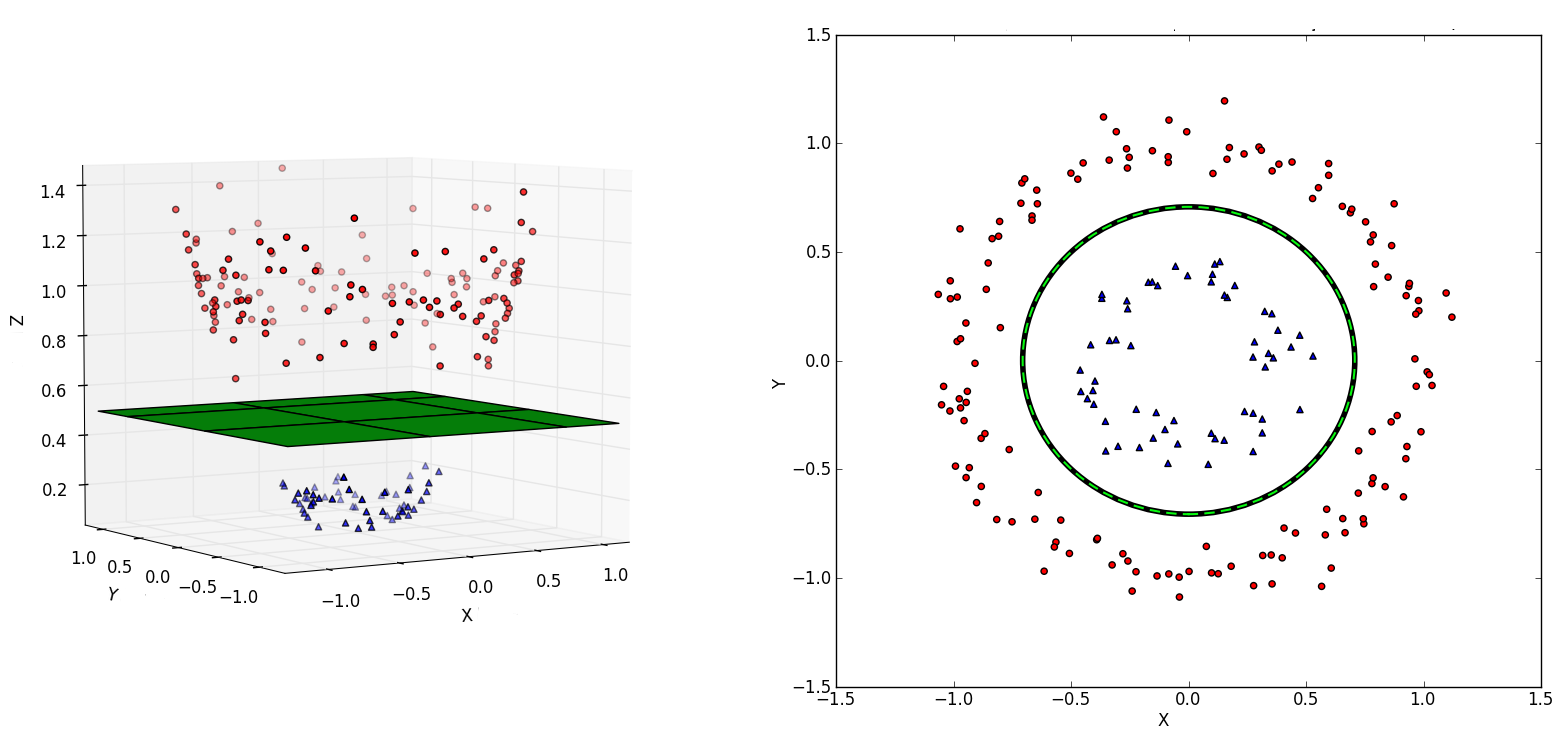
\includegraphics[width=1\textwidth]{svm2a.png}}%
	\caption{Hiperpłaszczyzna separująca w rozszerzonej przestrzeni cech (lewa strona). Rzut granicy decyzyjnej na pierwotną przestrzeń cech (prawa strona) \cite{svmimg}}
\end{figure}

W przypadku, gdy liczba klas do której mogą należeć obserwacje wynosi $k > 2$, trenuje się $k$ klasyfikatorów - po jednym na każdą klasę. Wtedy obserwacja jest zakwalifikowywana do tej klasy, której odpowiadający klasyfikator zwraca największą wartość \cite{islr}.

\chapter{Redukcja wymiarowości}
Redukcja wymiarowości jest procesem mającym na celu zmniejszenie liczby cech w zbiorze danych. Jeżeli przetwarzane dane mają bardzo wysoką wymiarowość, to uczenie klasyfikatorów oraz przeprowadzanie klasyfikacji może trwać nieakceptowalnie długo. Zbyt duża liczba cech niesie za sobą także ryzyko wzajemnej ich korelacji. Ponadto, duża liczba cech może być utrudnieniem w interpretacji modelu. Tematyka ta jest szeroko obecna w literaturze, gdyż skuteczność procesu klasyfikacji w dużym stopniu zależy od jakości przygotowanych danych (w tym zarówno selekcji cech jak i nadmiarowości) \cite{hall} \cite{verleysen} \cite{kotsiantis}.

Techniki redukcji wymiarowości można podzielić na dwie grupy: techniki selekcji cech oraz techniki ekstrakcji cech. Selekcja cech ma na celu pozbycie się ze zbioru danych cech nieistotnych. Ekstrakcja cech ma na celu przekształcenie wejściowego zestawu cech w inny, o niższej wymiarowości. Istnieje wiele metod redukcji wymiarowości danych, tj.: analiza czynnikowa, analiza składowych głównych, analiza skupień, analiza dyskryminacyjna \cite{fodor} \cite{dhavamany} \cite{tharwat} . Jedną z najbardziej popularnych technik redukcji wymiarowości, należącą do grupy selekcji cech, jest analiza składowych głównych (ang. \textit{Principal Component Analysis}, \textit{PCA}). Ze względu na to, iż metoda ta została zastosowana w eksperymentach prowadzonych w ramach niniejszej pracy zostanie ona omówiona poniżej, w kolejnym podrozdziale.

\section{Analiza składowych głównych}
Analiza składowych głównych polega na obliczeniu nowego zbioru cech, będącego kombinacją liniową cech pierwotnego zbioru danych, w taki sposób, aby maksymalizować wariancję każdej kolejnej cechy. Nowe cechy nazywane są składowymi głównymi (ang. \textit{Principal Components}). Składowe główne są wzajemnie nieskorelowane \cite{tharwat} \cite{joliffe} \cite{gewers}. 

Bardziej intuicyjnie, PCA polega na znalezieniu takiego kierunku w przestrzeni, dla którego wariancja rzutu chmury punktów na ten kierunek będzie możliwie największa. Następnie konstruuje się nowy układ współrzędnych, znajdując kolejne kierunki (ortogonalne do pierwszego) w taki sposób, aby maksymalizować wariancję rzutu chmury punktów dla każdego kolejnego kierunku \cite{tharwat} \cite{joliffe} \cite{gewers}. 

Niech $\mathbf{X}$ będzie macierzą $n \times p$, gdzie $n$ oznacza liczbę obserwacji, a $p$ oznacza liczbę cech. Poszukiwany jest wektor $\textbf{a} = [a_1,...,a_p]$ o długości równej 1, dla którego wariancja iloczynu $\mathbf{Xa}$ jest możliwie największa. Wariancja ta dana jest wzorem:
\begin{equation}
Var[\mathbf{Xa}] = \mathbf{a}^T\mathbf{Sa}
\end{equation}
gdzie $\mathbf{S}$ jest macierzą kowariancji macierzy danych $\mathbf{X}$. Maksymalna wartość wyrażenia (5.1), uwzględniając ograniczenie dotyczące jednostkowej długości wektora $\textbf{a}^T\textbf{a} = 1$, opisywana jest przez równanie (5.2) \cite{tharwat} \cite{joliffe}.
\begin{equation}
\mathbf{Sa} = \lambda \mathbf{a}
\end{equation}
Z równania (5.2) wynika, że $\mathbf{a}$ musi być wektorem własnym macierzy kowariancji $\mathbf{S}$, natomiast $\lambda$ jest odpowiadająca mu wartością własną. W szczególności poszukiwany jest wektor własny $\mathbf{a}_1$, któremu odpowiadająca wartość własna $\lambda_1$ jest największa, ponieważ wyznacza on kierunek maksymalnej wariancji. W ogólności wektory własne $\mathbf{a}_1, \mathbf{a}_2, ..., \mathbf{a}_p$, którym odpowiadają wartości własne $\lambda_1, \lambda_2, ..., \lambda_p$ spełniające zależność $ \lambda_1 \ge \lambda_2 \ge ... \ge \lambda_p$ wyznaczają kierunki kolejnych składowych głównych. Składowe główne można również obliczyć poprzez rozkład macierzy danych $\mathbf{X}$ według wartości osobliwych (ang. \textit{Singular Value Decomposition, SVD}) \cite{tharwat} \cite{joliffe} \cite{gewers}. 

Redukcja wymiarowości jest dokonywana poprzez pozostawienie w zbiorze danych pewnej liczby pierwszych składowych głównych i pozbycie się pozostałych. Operacja ta pokazana jest na rysunku 5.1. Liczba składowych głównych do pozostawienia może być zadeklarowana z góry. Innym możliwym podejściem jest zdefiniowanie części całkowitej wariancji początkowego zbioru danych, która ma być zachowana w ostatecznie wybranych składowych głównych. Wariancja zachowana przez $k$ pierwszych składowych głównych dana jest wzorem \cite{tharwat} \cite{joliffe} \cite{gewers}:
\begin{equation}
\frac{\sum_{i=1}^{k}\lambda_i}{\sum_{j=1}^{p}\lambda_j}, 1 \leq k \leq p
\end{equation}

\begin{figure}[H]
	\centering
	\makebox[\textwidth][c]{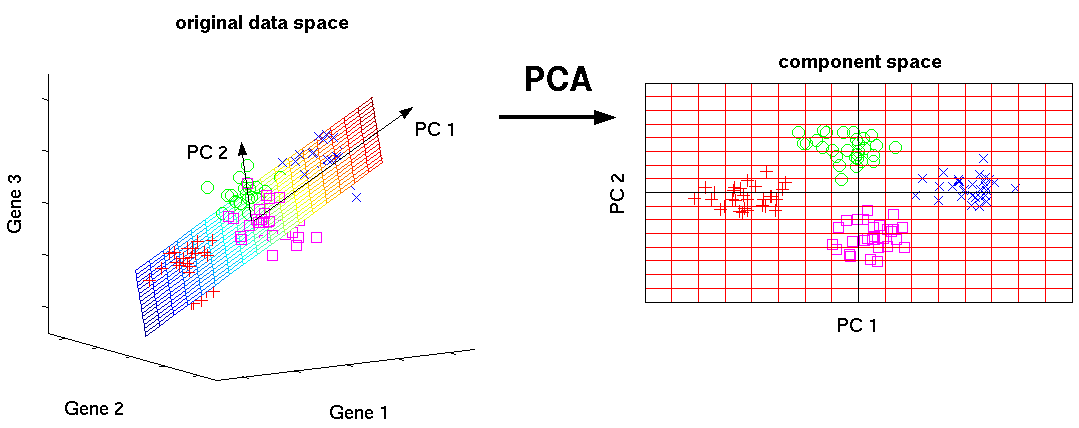
\includegraphics[width=1.1\textwidth]{pca_example.png}}%
	\caption{Wykres poziomów ekspresji 3 różnych genów dla obserwacji należących do 4 klas. PC1 i PC2 oznaczają kierunki odpowiednio pierwszej i drugiej składowej głównej (lewa strona). Wykres dwóch pierwszych składowych głównych (prawa strona) \cite{pca}}
\end{figure}



\chapter{Eksperymenty}
W ramach praktycznej części pracy przeprowadzono eksperymenty polegające na porównaniu skuteczności klasyfikacji danych testowych przy zastosowaniu wybranych metod parametryzacji sygnałów oraz klasyfikacji. Do przeprowadzenia eksperymentów użyto języka programowania Python w wersji 3.5. Najważniejsze użyte biblioteki to \textit{scikit-learn}, \textit{TensorFlow} oraz \textit{Keras} \cite{keras} \cite{sklearn} \cite{tensorflow}.

Podczas zajęć laboratoryjnych z przedmiotu \textit{Diagnostyka i protetyka słuchu i wzroku} zostały zarejestrowane sygnały EEG 17 osób biorących udział w zajęciach. W pierwszym etapie ćwiczenia polecono badanym osobom aby się zrelaksowały. W drugiej fazie badane osoby oglądnęły teledysk. W ostatnim etapie ćwiczenia badane osoby zagrały w grę wymagającą logicznego myślenia. Dla danej osoby każdy etap trwał tyle samo, jednakże długość pojedynczego etapu różniła się pomiędzy osobami. Do rejestracji sygnałów został użyty kask Emotiv EPOC+ wyposażony w 14 elektrod pomiarowych \cite{emotiv}. Częstotliwość próbkowania została ustawiona na wartość 128 Hz. Rejestracja sygnałów została przeprowadzona przez doktorantów Katedry Systemów Multimedialnych WETI PG i ten wątek nie należy do tematu niniejszej pracy magisterskiej.

W niniejszym rozdziale pracy zostały zawarte fragmenty kodu w języku Python. Są one uproszczonymi wersjami kodu wykorzystanego do obliczeń. Zostały zamieszczone w celu lepszego zobrazowania wykonywanych operacji.

\section{Opracowanie zbioru danych}
Wraz z zarejestrowanymi sygnałami został dostarczony skrypt napisany w języku Python. Skrypt automatycznie wycina ze zbioru danych pierwsze i ostatnie 50 sekund zarejestrowanych sygnałów, a także 50 sekund sygnałów zarejestrowanych pomiędzy kolejnymi etapami. Pozostałe sygnały są dzielone na ramki o zadanym czasie trwania. Każdej ramce przyporządkowywana jest odpowiednia kategoria: \textit{medytacja}, \textit{teledysk}, \textit{gra logiczna}.

Do oryginalnego skryptu została dodana możliwość podzielenia sygnałów danej kategorii z zakładką o zadanym czasie trwania. Zakładka polega na tym, że dla danej osoby $l$ ostatnich próbek danego kanału $i$-tej ramki danej kategorii ma takie same wartości, jak $l$ pierwszych próbek danego kanału $i+1$ ramki tej samej kategorii. Stosowanie zakładki ma na celu powiększenie zbioru danych. 

Ostatecznie zarejestrowane sygnały zostały pocięte na ramki o długości 1 s z zakładką 0.5 s. Pojedyncza ramka ma więc postać macierzy o wymiarach (128,14). Liczba wszystkich ramek wynosi 24795 - po 8265 na każdą kategorię.

\section{Przetwarzanie wstępne}
Opracowany zbiór danych został podzielony w losowy sposób na dane przeznaczone do uczenia, walidacji i testowania w proporcjach odpowiednio 70\%, 10\% i 20\%. Zostało to dokonane w następujący sposób:
\begin{lstlisting}
# podział danych na dane treningowe, walidacyjne oraz testowe
import random
data_train = {}, data_val = {}, data_test = {}
a = int(0.7  * 8265)
b = a + int(0.1 * 8265)
for class_name in eeg.keys(): # ['meditation','music_video','logic_game']
	indices = [i for i in range(8265)]
	random.shuffle(indices)
	data_train[class_name] = [eeg[class_name][i] for i in indices[:a]]
	data_val[class_name] = [eeg[class_name][i] for i in indices[a:b]]
	data_test[class_name] = [eeg[class_name][i] for i in indices[b:]]
\end{lstlisting}
W przypadku klasyfikatorów $k$-NN oraz SVM etap walidacji został pominięty, a dane przeznaczone na walidację zostały wykorzystane jako dane treningowe. 

Dla każdego z 14 kanałów w każdej ramce obliczono wartość średnią oraz wariancję próbek, co daje 28 wartości na ramkę. Zostały one zachowane do późniejszego wykorzystania.

Następnie z każdego z 14 kanałów w każdej ramce usunięto wartość średnią za pomocą funkcji \textit{scipy.signal.detrend}, po czym każda ramka została poddana operacji wybielenia i analizie składowych niezależnych (ICA, \textit{Independent Component Analysis}) z użyciem algorytmu FastICA.
\begin{lstlisting}
# analiza składowych głównych połączona z wybieleniem
# dla pojedynczej ramki
from sklearn.decomposition import FastICA
ica = FastICA(n_components=14, whiten=True)
new_dataframe = ica.fit_transform(dataframe)
\end{lstlisting}

\newpage
Następnie każdy kanał w każdej ramce został poddany parametryzacji metodami opisanymi poniżej, po czym wektory cech odpowiadające kolejnym kanałom zostały sklejone w jeden wektor cech. Ostatecznie, do otrzymanego w ten sposób wektora cech dołączone zostały wcześniej obliczone wartości średnie i wariancje. 

\begin{itemize}
	\item \textit{ar16} - na podstawie każdego kanału danej ramki za pomocą algorytmu Burga został obliczony model autoregresyjny rzędu 16. Wykorzystano do tego funkcję \textit{arburg} z biblioteki \textit{spectrum}. Z obliczonych cech wykorzystano jedynie części rzeczywiste (wszystkie części urojone miały wartość 0). Po złączeniu cech z poszczególnych kanałów oraz wartości średnich i wariancji powstały wektory cech o długości 252.
	\begin{lstlisting}
	# obliczanie modeli autoregresyjnych dla pojedynczej ramki
	import spectrum
	new_dataframe = []
	for channel in dataframe: 
		model = spectrum.arburg(channel,order=16,criteria=None)[0]
		model = [item.real for item in model]
		new_dataframe.append(model)
	\end{lstlisting}
	
	\item \textit{ar24} - tak jak \textit{ar16}, ale modele są rzędu 24. Wynikowe wektory cech mają długość 364.
	\item \textit{welch16} - na podstawie każdego kanału obliczana jest widmowa gęstość mocy za pomocą metody Welcha. Wykorzystano do tego funkcję \textit{welch} z biblioteki \textit{scipy}. Próbki z każdego kanału zostały podzielone na 8 mniejszych ramek, każda o długości 16. Na podstawie każdego kanału zostało obliczonych 9 współczynników. Wynikowe wektory cech mają długość 154.
	\begin{lstlisting}
	# obliczanie widmowej gęstości mocy metodą Welcha 
	# dla pojedynczej ramki
	import scipy.signal
	psd = scipy.signal.welch(dataframe,nperseg=16,axis=0)[1]
	\end{lstlisting}
	
	\item \textit{welch32} - tak jak \textit{welch16}, ale ramki zostały podzielone na 4 krótsze ramki, każda po 32 próbki na kanał. Wynikowe wektory cech mają długość 266.
	\item \textit{welch64} - tak jak \textit{welch16} i \textit{welch32}, ale ramki zostały podzielone na 2 krótsze ramki, każda po 64 próbki na kanał. Wynikowe wektory cech mają długość 490.
	\item \textit{dwt} - każdy kanał został poddany 4-poziomowej dyskretnej transformacji falkowej z użyciem falki \textit{db4}. Użyto do tego funkcji \textit{wavedec} z biblioteki \textit{pywt}. Zwrócone wektory współczynników falkowych maja długości kolejno: 14,14,22,37,67. Po złączeniu wszystkich wektorów współczynników falkowych dla wszystkich kanałów w jeden wektor cech i dodaniu wartości średnich oraz wariancji wynikowe wektory cech mają długość 2184.
	\begin{lstlisting}
	# obliczanie dyskretnej transformacji falkowej 
	# dla pojedynczej ramki
	import pywt, numpy as np
	new_dataframe = []
	for channel in dataframe:
		dwt = pywt.wavedec(channel,wavelet="db4",level=4,axis=0)
		vector = np.ndarray((0,))
		for item in dwt:
			vector = np.append(vector,item)
		new_dataframe.append(vector)
	\end{lstlisting}
	
	\item \textit{dwt\_stat} - każdy kanał zostaje poddany dyskretnej transformacji falkowej z parametrami takimi jak w metodzie \textit{dwt}. Następnie dla każdego z 5 wektorów współczynników falkowych obliczane są parametry: wartość średnia, wartość średnia z wartości bezwzględnych,  wariancja, skośność, kurtoza, liczba przejść przez zero oraz suma kwadratów współczynników.
	\begin{lstlisting}
	# obliczanie parametrów opisowych ze współczynników 
	# falkowych dla pojedynczej ramki
	import numpy as np, scipy.stats, pywt
	def zero_crossings(data):
		return ((data[:-1] * data[1:]) < 0).sum()
	dwt = pywt.wavedec(channel,wavelet="db4",level=4,axis=0)
	vector = []
	for item in dwt:
		vector.append(np.mean(item))
		vector.append(np.mean(np.abs(item)))
		vector.append(np.var(item))
		vector.append(scipy.stats.skew(item))
		vector.append(scipy.stats.kurtosis(item))
		vector.append(zero_crossings(item))
		vector.append(sum(np.power(item,2)))
	\end{lstlisting}
\end{itemize}

Wymiarowość wektorów cech dla każdej metody parametryzacji została następnie zredukowana poprzez dokonanie analizy składowych głównych na zbiorze danych treningowych w taki sposób, aby zachować 95\% wariancji w zbiorze danych treningowych. Następnie wszystkie pozostałe dane są rzutowane do pozyskanego w wyniku PCA układu współrzędnych.
\begin{lstlisting}
# redukcja wymiarowości danych poprzez analizę składowych głównych
from sklearn.decomposition import PCA
pca = PCA(n_components=0.95)
pca.fit(train_data)
reduced_train_data = pca.transform(train_data)
reduced_val_data = pca.transform(val_data)
reduced_test_data = pca.transform(test_data)
\end{lstlisting}
Należy zaznaczyć, że dla każdej metody parametryzacji zostały opracowane dwa różne docelowe układy współrzędnych. W przypadku klasyfikatorów $k$-NN oraz SVM etap walidacji został pominięty - dane walidacyjne zostały wykorzystane jako dane treningowe. Tak więc, dla klasyfikatorów $k$-NN i SVM analiza składowych głównych wykonywana jest na podstawie 80\% danych, natomiast dla sieci neuronowych na podstawie 70\% danych. Po redukcji wymiarowości długości wektorów cech dla poszczególnych metod parametryzacji wyniosły odpowiednio: 
\begin{itemize}
	\item \textit{ar16} - 38 w obydwu przypadkach
	\item \textit{ar24} - 61 w obydwu przypadkach
	\item \textit{welch16} - 61 w obydwu przypadkach
	\item \textit{welch32} - 110 w obydwu przypadkach
	\item \textit{welch64} - 204 w obydwu przypadkach
	\item \textit{dwt} - 1019 dla $k$-NN i SVM, 1016 dla sieci neuronowych
	\item \textit{dwt\_stat} - 136 w obydwu przypadkach
\end{itemize}

W przypadku trenowania sieci neuronowych wymagane jest, aby wejścia i wyjścia sieci były zakodowane w postaci wektorów liczb. Poniżej pokazano sposób kodowania klas metodą \textit{one-hot encoding}.

\begin{lstlisting}
# kodowanie klas metodą one-hot encoding
classes = {}
classes['meditation'] = np.array([1,0,0])
classes['music_video'] = np.array([0,1,0])
classes['logic_game'] = np.array([0,0,1])
for i in range(len(train_data_classes)):
train_data_classes[i] = classes[train_data_classes[i]]
for i in range(len(test_data_classes)):
test_data_classes[i] = classes[test_data_classes[i]]
for i in range(len(val_data_classes)):
val_data_classes[i] = classes[val_data_classes[i]]
\end{lstlisting}

\section{Eksperyment nr 1: $k$-najbliższych sąsiadów}
W ramach pierwszego eksperymentu wytrenowano klasyfikatory $k$-NN dla wybranych wartości $k$ z użyciem 80\% danych. Pozostałe 20\% danych użyto do przetestowania klasyfikatorów. W roli miary wyniku użyto stosunku liczby poprawnie zaklasyfikowanych ramek testowych do liczby wszystkich ramek testowych. Poniżej przedstawiono sposób uczenia klasyfikatorów, klasyfikacji danych testowych, obliczania dokładności klasyfikacji, macierzy błędów, precyzji, czułości oraz miary $F_1$.

\begin{lstlisting}
# uczenie klasyfikatora k-NN, klasyfikacja danych testowych,
# obliczanie dokładności klasyfikacji, macierzy błędów,
# precyzji, czułości oraz miary F1
from sklearn.neighbors import KNeighborsClassifier
from sklearn.metrics import accuracy_score, confusion_matrix, classification_report
knn = KNeighborsClassifier(k_neighbors=k)
knn.fit(reduced_train_data,train_data_classes)
results = knn.transform(reduced_test_data)
score = accuracy_score(test_data_classes,results)
conf_matrix = confusion_matrix(test_data_classes,results)
report = classification_report(test_data_classes,results)
\end{lstlisting}

Wyniki przedstawiono w tablicy 6.1. Najlepsze wyniki indywidualne dla danej metody parametryzacji oraz najlepszy spośród wyników średnich ze wszystkich metod parametryzacji dla danej wartości $k$ zaznaczono kolorem niebieskim. Najlepszy ze wszystkich wynik indywidualny oraz najlepszy wynik średni ze wszystkich wartości $k$ dla danej metody parametryzacji zaznaczono kolorem czerwonym.

 \begin{table}[H]
	\centering
	\small
	\setlength\tabcolsep{2pt}
	\begin{tabular}{ | c | c | c | c | c | c | c | c !{\vline width 1pt} c |}
		\hline
		& \multicolumn{6}{c}{Metoda parametryzacji} & & \\ \hline
		 $k$ & \textit{ar16}  & \textit{ar24} & \textit{dwt} & \textit{dwt\_stat} & \textit{welch16} & \textit{welch32} & \textit{welch64}  & \textbf{\textit{średnia}} \\ \hline
		 5 & 0.4742 &  0.4605 & 0.3529 & 0.4192 & 0.5999 & 0.6304 & 0.6052 & 0.5060 \\ \hline
		 7 & 0.4891 & 0.4756 & 0.3559 &  0.4327 & 0.6084 & 0.6338 & 0.6145 & 0.5010 \\ \hline
		 11 & 0.4941 & 0.4875 & 0.3535 & 0.4403 & 0.6163 & \color{red} 0.6386 & 0.6245 & 0.5157 \\ \hline
		 14 & 0.5030 & 0.4927 & 0.3533 & 0.4456 & \color{blue} 0.6141 & 0.6370 & \color{blue} 0.6358 & 0.5259  \\ \hline
		 17 & \color{blue} 0.5066 & \color{blue} 0.4998 & \color{blue} 0.3563 & \color{blue} 0.4569 & 0.6129 & 0.6362 & 0.6322 & \color{blue} 0.5287  \\ \Xhline{1pt}
		 \textbf{\textit{średnia}} & 0.4934 & 0.4832 & 0.3544 & 0.4389 & 0.6103 & \color{red}0.6352 & 0.6224 &\\ \hline

	\end{tabular}
	\caption{Wyniki klasyfikacji ramek testowych za pomocą klasyfikatorów $k$-NN dla wybranych wartości $k$.}
\end{table} 


W wykonanym eksperymencie najlepszą dokładność klasyfikacji osiągnięto dla metody \textit{welch32} w połączeniu z wartością $k = 11$ - wyniosła ona 63.86\%. Również średnia dokładność klasyfikacji ze wszystkich wartości $k$ jest największa dla metody \textit{welch32}. W ogólności metoda Welcha okazała się być zdecydowanie najlepszą metodą parametryzacji. Wszystkie jej zastosowane warianty sprawdziły się znacząco lepiej, niż pozostałe metody parametryzacji. Warianty \textit{welch32} i \textit{welch64} sprawdziły się nieco lepiej, niż wariant \textit{welch16}, zarówno biorąc pod uwagę wyniki średnie, jak i najlepsze. Wszystkie warianty metody Welcha poskutkowały jednak średnią dokładnością klasyfikacji większą niż 60\%. Żadna inna metoda parametryzacji nie zbliżyła się nawet do tego wyniku.

Do progu 50\% średniej poprawności klasyfikacji zbliżyły się warianty modelowania autoregresyjnego \textit{ar16} oraz \textit{ar24}. Co interesujące, zastosowanie wariantu \textit{ar24} skutkowało nieco mniejszą dokładnością klasyfikacji, niż zastosowanie wariantu \textit{ar16}. Pokazuje to, że zwiększanie wymiarowości wektora cech nie zapewnia wyższej dokładności klasyfikacji.
	
Zaskakująco słabo wypadły metody falkowe. Wariant \textit{dwt} okazał się być najmniej skuteczną metodą parametryzacji w tym zestawieniu. Nieco lepiej, choć nadal słabo, wypadł wariant \textit{dwt\_stat}. Jednym z powodów słabych wyników uzyskanych w przypadku wariantu \textit{dwt} może być zbyt wysoka wymiarowość wektorów cech. Jest to szczególnie problematyczne w przypadku klasyfikatora $k$-NN, o czym wspomniano w rozdziale 4.

W przypadku metod autoregresyjnych i falkowych najlepsze rezultaty osiągnięto dla najwyższej użytej wartości parametru $k$ wynoszącej 17. Metoda Welcha lepiej sprawdziła się z wartościami $k$ wynoszącymi 11 oraz 14. Należy jednak zaznaczyć, że wpływ przetestowanych wartości parametru $k$ na dokładność klasyfikacji okazał się być niewielki w porównaniu do wpływu metody parametryzacji.

\begin{figure}[H]
	\begin{minipage}{0.48\textwidth}
		\centering
		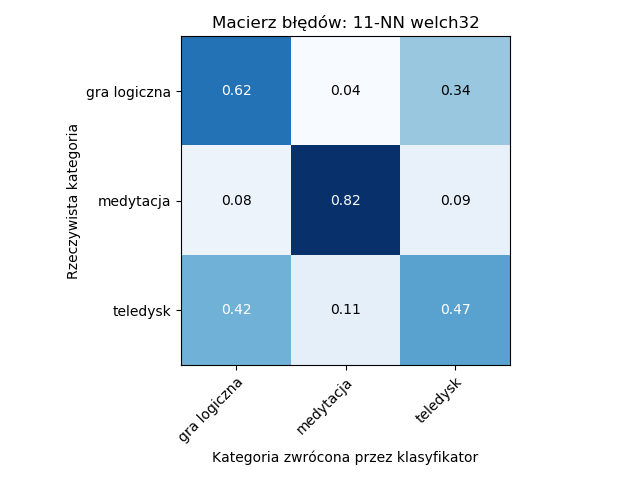
\includegraphics[width=1.3\linewidth]{11nn_welch_32_cm.png}
	\end{minipage}
	\begin{minipage}{0.48\textwidth}
		\centering
		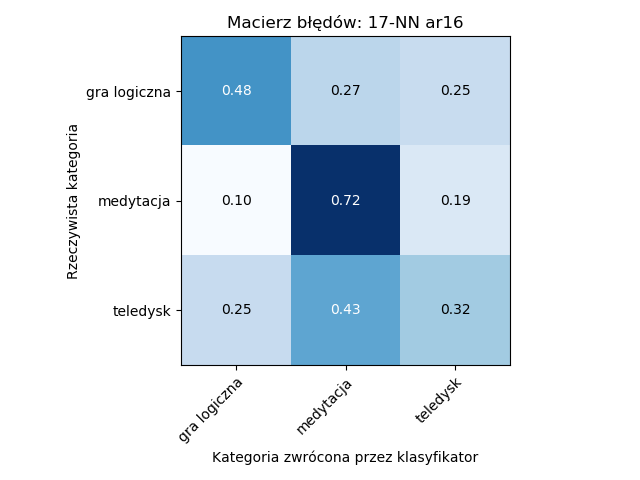
\includegraphics[width=1.3\linewidth]{17nn_ar_16_cm.png}
	\end{minipage}
	\caption{Znormalizowana macierz błędów dla klasyfikatora 11-NN i metody parametryzacji \textit{welch32} (lewa strona). Znormalizowana macierz błędów dla klasyfikatora 17-NN i metody parametryzacji \textit{ar16} (prawa strona).}
\end{figure}

Po lewej stronie rysunku 6.1 przedstawiono znormalizowaną macierz błędów dla klasyfikatora 11-NN i metody parametryzacji \textit{welch32}. Jak widać, ramki należące do kategorii \textit{medytacja} zostały w większości prawidłowo zaklasyfikowane, natomiast ramki kategorii \textit{gra logiczna} i \textit{teledysk} były ze sobą często mylone. Jest to poniekąd oczekiwany wynik - zarówno oglądanie teledysku, jak i rozwiązywanie zagadek logicznych powodują pewne pobudzenie umysłowe i wymagają koncentracji uwagi. Medytacja, jako czynność najbardziej odmienna od pozostałych, okazała się najłatwiejsza do poprawnej klasyfikacji. Macierze błędów dla 11-NN i \textit{welch16} oraz 11-NN i \textit{welch64} (nie zostały przedstawione w pracy ze względu na ograniczoną długość pracy) zawierają bardzo podobne wartości.

Po prawej stronie rysunku 6.1 przedstawiono znormalizowaną macierz błędów dla klasyfikatora 17-NN i metody parametryzacji \textit{ar16}. I w tym przypadku ramki należące do kategorii \textit{medytacja} są w większości przyporządkowywane poprawnie. Ramki klasy \textit{gra logiczna} są niekiedy przyporządkowywane do dwóch pozostałych klas. Ramki klasy \textit{teledysk} są najrzadziej poprawnie klasyfikowane - jedynie 32\% ramek tej klasy zostało przypisane do właściwej kategorii. Aż 43\% ramek z kategorii \textit{teledysk} zostało zaklasyfikowanych do kategorii \textit{medytacja}. Macierz błędów dla wariantu 17-NN \textit{ar24} (nie przedstawiona w pracy) zawiera bardzo podobne wartości.

Na rysunku 6.2 przedstawiono znormalizowane macierze błędów dla wariantów odpowiednio 11-NN \textit{dwt} i 11-NN \textit{dwt\_stat}. Macierze te bardzo się od siebie różnią. W wariancie \textit{dwt} większość ramek ze wszystkich klas została zaklasyfikowana jako \textit{gra logiczna}, znacznie mniejsza część jako \textit{teledysk} i znikoma część jako \textit{medytacja}. W wariancie \textit{dwt\_stat} ramki klasy \textit{medytacja} zostały w większości poprawnie zaklasyfikowane, natomiast ramki klas \textit{gra logiczna} oraz \textit{teledysk} zostały przyporządkowane w różnych proporcjach do wszystkich klas, najczęściej jednak do klasy \textit{medytacja}.

\begin{figure}[H]
	\begin{minipage}{0.48\textwidth}
		\centering
		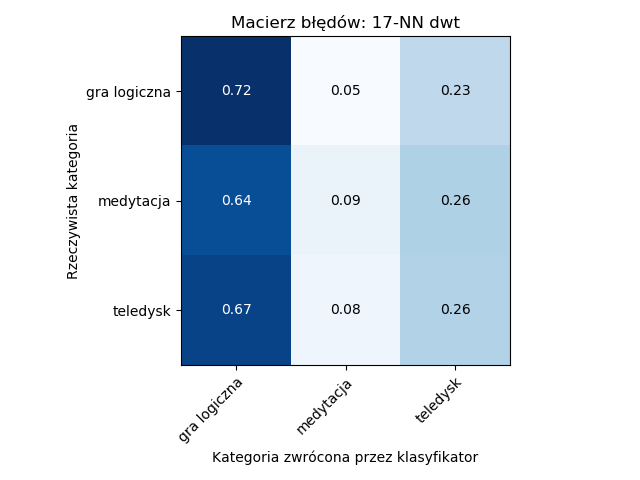
\includegraphics[width=1.3\linewidth]{17nn_dwt_cm.png}
	\end{minipage}
	\begin{minipage}{0.48\textwidth}
	\centering
	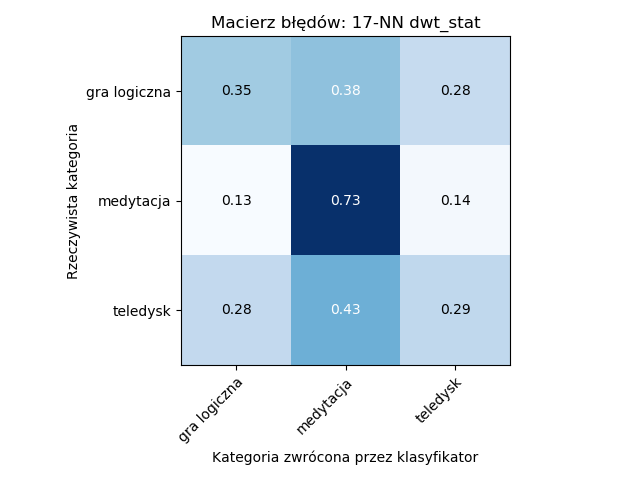
\includegraphics[width=1.3\linewidth]{17nn_dwt_2_cm.png}
	\end{minipage}
	\caption{Znormalizowana macierz błędów dla klasyfikatora 17-NN i metody parametryzacji \textit{dwt} (lewa strona). Znormalizowana macierz błędów dla klasyfikatora 17-NN i metody parametryzacji \textit{dwt\_stat} (prawa strona).}
\end{figure}

W tablicy 6.2 przedstawiono wartości prezycji, czułości oraz miary $F_1$ dla tych wariantow eksperymentu, dla których wykreślono macierze błędów. Precyzja dla danej klasy definiowana jest jako stosunek liczby ramek tej klasy poprawnie zaklasyfikowanych do sumy liczby wszystich ramek zaklasyfikowanych do klasy $x$. Czułość dla danej klasy definiowana jest jako iloraz liczby ramek tej klasy poprawnie zaklasyfikowanych do liczby wszystkich ramek należących do tej klasy. Miara $F_1$ dla danej klasy definiowana jest następująco: 
\begin{equation}
F_1 = 2 \cdot \frac{\text{precyzja} \cdot \text{czułość}}{\text{precyzja}+\text{czułość}} 
\end{equation}

 \begin{table}[H]
	\centering
	\small
	\setlength\tabcolsep{2pt}
	\begin{tabular}{| c | c | c | c | c |}
		\hline
		Wariant & Klasa & Precyzja  & Czułość & Miara $F_1$ \\ \hline
		\multirow{3}{*}{11-NN \textit{welch32}} & \textit{medytacja} & 0.8497 & 0.8234 & 0.8363  \\ 
		& \textit{gra logiczna} & 0.5521 & 0.6215 & 0.5847  \\ 
		& \textit{teledysk} & 0.5204 & 0.4710 & 0.4944 \\ \hline
		\multirow{3}{*}{17-NN \textit{ar16}} & \textit{medytacja} & 0.5049 & 0.7177 & 0.5928 \\
		& \textit{gra logiczna} & 0.5824 & 0.4807 & 0.5267\\
		& \textit{teledysk} & 0.4270 & 0.3216 & 0.3669\\ \hline
		\multirow{3}{*}{17-NN \textit{dwt}} & \textit{medytacja} & 0.4274 & 0.0925 & 0.1521 \\
		& \textit{gra logiczna} & 0.3545 & 0.7201 & 0.4751\\
		& \textit{teledysk} & 0.3408 & 0.2563 & 0.2926\\ \hline
		\multirow{3}{*}{17-NN \textit{dwt\_stat}} & \textit{medytacja} & 0.4772 & 0.7334 & 0.5782 \\
		& \textit{gra logiczna} & 0.4593 & 0.3476 & 0.3957\\
		& \textit{teledysk} & 0.4101 & 0.2896 & 0.3395\\ \hline
	\end{tabular}
	\caption{Wartości precyzji, czułości oraz miary $F_1$ dla każdej z klas dla metod parametryzacji \textit{welch32}, \textit{ar16}, \textit{dwt} oraz \textit{dwt\_stat}.}
\end{table} 

\section{Eksperyment nr 2: maszyny wektorów nośnych z liniową funkcją rdzenia}
W ramach drugiego eksperymentu sprawdzono dokładność klasyfikacji za pomocą maszyn wektorów nośnych. W roli funkcji rdzenia wykorzystano funkcję liniową. Użyte wartości parametru $C$ wynoszą $0.01$, $0.1$, $1$, $10$, $100$. Dla niektórych kombinacji metod parametryzacji i wartości parametru $C$ nie wykonano testów ze względu na bardzo długie czasy uczenia klasyfikatorów połączone z niskimi wartościami wyników w wykonanych wariantach tego eksperymentu oraz eksperymentu nr 1. Użyte dane treningowe, testowe oraz miara wyniku są takie same, jak w eksperymencie nr 1. Poniżej przedstawiono sposób trenowania klasyfikatorów oraz klasyfikacji danych testowych.

\begin{lstlisting}
# uczenie klasyfikatora SVM z liniową funkcją rdzenia
# oraz klasyfikacja danych testowych
from sklearn.svm import SVC
svm = SVC(C=C,kernel='linear')
svm.fit(reduced_train_data,train_data_classes)
results = svm.transform(reduced_test_data)
\end{lstlisting}

Wyniki przedstawiono w tablicy 6.3. Najlepsze wyniki indywidualne dla danej metody parametryzacji oraz najlepszy spośród wyników średnich ze wszystkich metod parametryzacji dla danych wartości $C$ zaznaczono kolorem niebieskim. Najlepsze ze wszystkich wyniki indywidualne oraz najlepszy wynik średni ze wszystkich wartości $C$ dla danej metody parametryzacji zaznaczono kolorem czerwonym.

\begin{table}[H]
	\centering
	\small
	\setlength\tabcolsep{2pt}
	\begin{tabular}{| c | c | c | c | c | c | c | c !{\vline width 1pt} c |}
		\hline
		& \multicolumn{6}{c}{Metoda parametryzacji} & & \\ \hline
		$C$ & \textit{ar16}  & \textit{ar24} & \textit{dwt} & \textit{dwt\_stat} & \textit{welch16} & \textit{welch32} & \textit{welch64}  & \textbf{\textit{średnia}} \\ \hline
		0.01 & 0.5072 & \color{blue} 0.5397 & \color{blue} 0.3353 & \color{blue} 0.5149 & 0.5653 & 0.6122 & 0.6290 & 0.5291 \\ \hline
		0.1 & 0.5083 & \color{blue} 0.5397 & 0.3351 & 0.5129 & 0.6070 & 0.6378 & 0.6528 & 0.5491 \\ \hline
		1 & \color{blue} 0.5085 & 0.5393 & 0.3287 & 0.5131 & 0.6249 & \color{red} 0.6671 & \color{blue} 0.6612 & 0.5490 \\ \hline
		10 & \color{blue} 0.5085 & 0.5395 & - & 0.5145 & \color{blue} 0.6550 & 0.6628 & 0.6598 & 0.5900  \\ \hline
		100 & \color{blue} 0.5085 & \color{blue} 0.5397 & - & - & 0.6548 & 0.6638 & 0.6548 & \color{blue} 0.6043 \\ \Xhline{1pt}
		\textbf{\textit{średnia}} & 0.5082 & 0.5396 & 0.3330 & 0.5138 & 0.6214 & 0.6487 & \color{red} 0.6515 & \\ \hline
	\end{tabular}
	\caption{Wyniki klasyfikacji ramek testowych za pomocą klasyfikatorów SVM z liniową funkcją rdzenia dla wybranych wartości $C$.}
\end{table} 

W przypadku liniowej funkcji rdzenia najlepszą dokładność klasyfikacji uzyskano dla metody parametryzacji \textit{welch32} i wartości $C=1$, podobnie jak w eksperymencie nr 1. Wyniosła ona 66.71\%, czyli prawie o 3 punkty procentowe więcej niż najlepszy wynik w eksperymencie nr 1. Najlepszą średnią dokładność klasyfikacji uzyskano dla metody parametryzacji \textit{welch64}, chociaż wariant \textit{welch32} sprawdził się w podobnym stopniu. Najwyższe wyniki średnie po wszystkich metodach parametryzacji uzyskano dla $C=10$ oraz $C=100$. Jest to zapewne spowodowane nieprzeprowadzeniem eksperymentu z wyżej wymienionymi wartościami $C$ dla falkowych metod parametryzacji, co zawyża wartości średnie wyników.

Zarówno najlepsze, jak i średnie wyniki klasyfikacji okazały się być nieco wyższe, niż w eksperymencie nr 1. Niemniej jednak z obu eksperymentów można wyciągnąć podobne wnioski. Metoda Welcha ponownie okazała się być najlepszą metodą parametryzacji, zarówno pod względem maksymalnych, jak i średnich wyników. Metoda parametryzacji \textit{dwt} ponownie okazała się być najmniej skuteczną. Główna różnica polega na tym, że wariant \textit{ar24} tym razem okazał się być bardziej skuteczny, niż wariant \textit{ar16}. Dla wariantu \textit{dwt\_stat} zanotowano największą poprawę wyników klasyfikacji w stosunku do eksperymentu nr 1.

Na rysunkach 6.3 oraz 6.4 przedstawiono znormalizowane macierze błędów dla metod parametryzacji \textit{welch32}, \textit{ar16}, \textit{dwt} oraz \textit{dwt\_stat}. Dla pierwszych trzech wymienionych wariantów rozkład błędów jest bardzo podobny do rozkładu błędów z eksperymentu nr 1. Dla wariantu \textit{dwt\_stat} można zauważyć poprawę dokładności klasyfikacji ramek kategorii \textit{gra logiczna} oraz \textit{teledysk} w porównaniu do eksperymentu nr 1.

\begin{figure}[H]
	\begin{minipage}{0.48\textwidth}
		\centering
		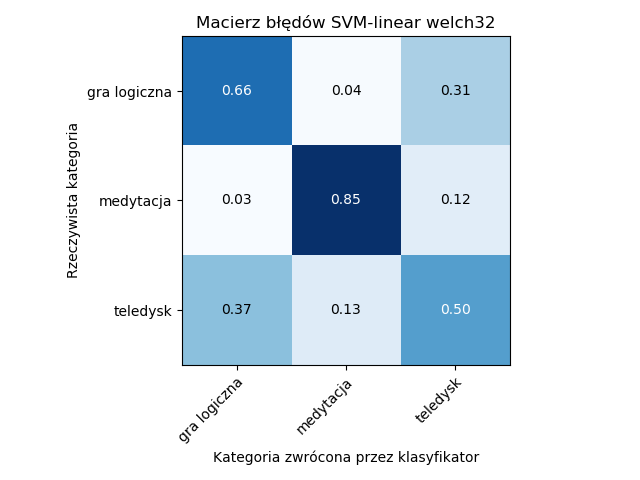
\includegraphics[width=1.3\linewidth]{linear_svm_welch_32_cm2.png}
	\end{minipage}
	\begin{minipage}{0.48\textwidth}
		\centering
		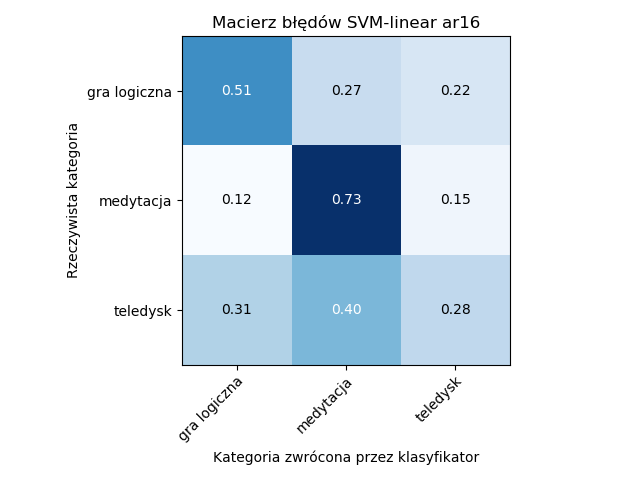
\includegraphics[width=1.3\linewidth]{linear_svm_ar_16_cm2.png}
	\end{minipage}
	\caption{Znormalizowana macierz błędów dla klasyfikatora SVM z liniową funkcją rdzenia i wartością $C=1$ oraz metody parametryzacji \textit{welch32} (lewa strona). Znormalizowana macierz błędów dla klasyfikatora SVM z liniową funkcją rdzenia i wartością $C=1$ oraz metody parametryzacji \textit{ar16} (prawa strona).}
\end{figure}

\begin{figure}[H]
	\begin{minipage}{0.48\textwidth}
		\centering
		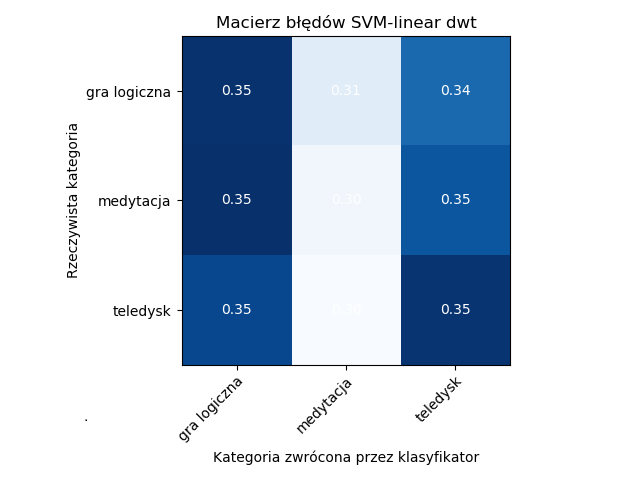
\includegraphics[width=1.3\linewidth]{linear_svm_dwt_cm2.png}
	\end{minipage}
	\begin{minipage}{0.48\textwidth}
		\centering
		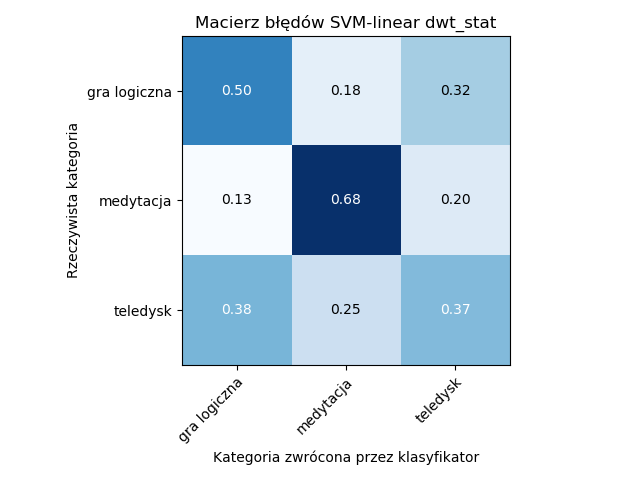
\includegraphics[width=1.3\linewidth]{linear_svm_dwt_2_cm2.png}
	\end{minipage}
	\caption{Znormalizowana macierz błędów dla klasyfikatora SVM z liniową funkcją rdzenia i wartością $C=0.01$ oraz metody parametryzacji \textit{dwt} (lewa strona). Znormalizowana macierz błędów dla klasyfikatora SVM z liniową funkcją rdzenia oraz wartością $C=0.01$ i metody parametryzacji \textit{dwt\_stat} (prawa strona).}
\end{figure}

W tablicy 6.4 przedstawiono wartości precyzji, czułości oraz miary $F_1$ dla metod parametryzacji \textit{welch32}, \textit{ar16}, \textit{dwt} oraz \textit{dwt\_stat}. We wszyskich wariantach za wyjątkiem \textit{dwt} wartości wszystkich miar są najwyższe dla klasy \textit{medytacja}, a najniższe dla klasy \textit{teledysk}.

\begin{table}[H]
	\centering
	\small
	\setlength\tabcolsep{2pt}
	\begin{tabular}{| c | c | c | c | c |}
		\hline
		Wariant & Klasa & Precyzja  & Czułość & Miara $F_1$ \\ \hline
		\multirow{3}{*}{} \textit{welch32} & \textit{medytacja} & 0.8369 & 0.8501 & 0.8434 \\
		C = 1 & \textit{gra logiczna} & 0.6179 & 0.6560 & 0.6364 \\
		& \textit{teledysk} & 0.5367 & 0.4952 & 0.5151 \\ \hline
		\multirow{3}{*}{} \textit{ar16} & \textit{medytacja} & 0.5209 & 0.7310 & 0.6083 \\
		C = 1 & \textit{gra logiczna} & 0.5400 & 0.5103 & 0.5247 \\
		& \textit{teledysk} & 0.4360 & 0.2842 & 0.3441 \\ \hline
		\multirow{3}{*}{} \textit{dwt} & \textit{medytacja} & 0.3324 & 0.3017 & 0.3163 \\
		C = 0.01 & \textit{gra logiczna} & 0.3345 & 0.3525 & 0.3432\\
		& \textit{teledysk} & 0.3388 & 0.3519 & 0.3452\\ \hline
		\multirow{3}{*}{} \textit{dwt\_stat} & \textit{medytacja} & 0.6134 & 0.6753 & 0.6429 \\
		C = 0.01 & \textit{gra logiczna} & 0.4946 & 0.5000 & 0.4973 \\
		& \textit{teledysk} & 0.4159 & 0.3694 & 0.3913 \\ \hline
	\end{tabular}
	\caption{Wartości precyzji, czułości oraz miary $F_1$ dla każdej z klas dla wybranych wariantów eksperymentu nr 2.}
\end{table} 

\section{Eksperyment nr 3: maszyny wektorów nośnych z radialną funkcją rdzenia}

Eksperyment nr 2 powtórzono stosując radialne funkcje bazowe w roli funkcji rdzenia. Użyte wartości parametru $\gamma$ wynoszą $0.1$, $1$, $10$. Poniżej przedstawiono sposób trenowania klasyfikatorów oraz klasyfikacji danych testowych. Wyniki przedstawiono w tablicy 6.5.

\begin{lstlisting}
# uczenie klasyfikatora SVM z radialną funkcją rdzenia
# oraz klasyfikacja danych testowych
from sklearn.svm import SVC
svm = SVC(C=C,kernel='rbf',gamma=gamma)
svm.fit(reduced_train_data,train_data_classes)
results = svm.transform(reduced_test_data))
\end{lstlisting}

W przypadku zastosowania radialnych funkcji bazowych największa indywidualną dokładność klasyfikacji ponownie została osiągnięta dla wariantu \textit{welch32} z parametrami $C = 10$ oraz $\gamma = 10$. Dokładność ta wyniosła 69.33\%, co jest wynikiem lepszym o ponad 2.5 punktu procentowego w porównaniu do najlepszego wyniku dla liniowej funkcji rdzenia, oraz o 5.5 punktu procentowego lepszym w porównaniu do klasyfikatora $k$-NN. Tak jak w poprzednich eksperymentach, wyniki uzyskane przy zastosowaniu metody Welcha - w szczególności w wariantach  \textit{welch32} i \textit{welch64} - okazały się być znacznie wyższe, niż przy zastosowaniu pozostałych metod parametryzacji. 

\begin{table}[H]
	\centering
	\small
	\setlength\tabcolsep{2pt}
	\begin{tabular}{| c | c | c | c | c | c | c | c | c !{\vline width 1pt} c |}
		\hline
		\multicolumn{2}{|c|}{} & \multicolumn{6}{c}{Metoda parametryzacji} & & \\ \hline
		$C$ & $\gamma$ & \textit{ar16}  & \textit{ar24} & \textit{dwt} & \textit{dwt\_stat} & \textit{welch16} & \textit{welch32} & \textit{welch64}  & \textbf{\textit{średnia}} \\ \Xhline{1pt}
		\multirow{3}{*}{0.01} & 0.1 & 0.3769 & 0.3392 & 0.4097 & \color{blue} 0.3976 & 0.5651 & 0.6133 & 0.6231 & 0.4750 \\
		& 1 & 0.3333 & 0.3333 & 0.3414 & 0.3523 & 0.5689 & 0.6193 & 0.6332 & 0.4545 \\
		& 10 & 0.4252 & 0.4180 & 0.3557 & 0.3333 & 0.6072 & 0.6378 & 0.6380 & 0.4879 \\ \Xhline{1pt}
		\multirow{3}{*}{0.1} & 0.1 & 0.4821 & 0.3734 & 0.4097 &  \color{blue} 0.3976 & 0.5651 & 0.6169 & 0.6310 & 0.4965 \\
		& 1 &0.3333 & 0.3333 & 0.3392 & 0.3529 & 0.6161 & 0.6453 &  0.6578 & 0.4683 \\
		& 10 & 0.4252 & 0.4178 & 0.3557 & 0.3333 & 0.6334 & 0.6683 & 0.6713 & 0.5007 \\ \Xhline{1pt}
		\multirow{3}{*}{1} & 0.1 & \color{blue} 0.5286 & \color{blue} 0.5107 & 0.4222 & 0.3333 & 0.6157 & 0.6455 & 0.6604 & 0.5309 \\
		& 1 & 0.3597 & 0.3333 & \color{blue} 0.4319 & 0.3535 & 0.6338 & 0.6655 & 0.6709 & 0.4927 \\
		& 10 & 0.3333 & 0.4178 & 0.3557 & 0.3333 & 0.6578 & 0.6846 & \color{blue} 0.6866 & 0.4956 \\ \Xhline{1pt}
		\multirow{3}{*}{10} & 0.1 & 0.4998 &  0.5070 & - & 0.3535 & 0.6334 & 0.6650 & 0.6626 & 0.5535 \\
		& 1 & 0.3636 & 0.3366 & - & 0.3333 & 0.6578 & 0.6681 & 0.6765 & 0.5060 \\
		& 10 & 0.3333 & 0.4210 & - & - & 0.6632 & \color{red} 0.6933 & 0.6644 & \color{blue} 0.5550 \\ \hline
		\multirow{3}{*}{100} & 0.1 & 0.5000 & - & - & 0.3327 & 0.6133 & 0.6632 & 0.6626 & 0.5544 \\
		& 1 & 0.3636 & - & - & 0.3535 & 0.6548 & 0.6820 & 0.6725 & 0.5453 \\
		& 10 & 0.3333 & - & - & 0.3333 & \color{blue} 0.6683 & 0.6701 & 0.6606 & 0.5331 \\ \Xhline{1pt}
		\multicolumn{2}{|c|}{\textbf{\textit{średnia}}} & 0.3994 & 0.3951 & 0.3801 & 0.3495 & 0.6236 & 0.6559 & \color{red} 0.6581 & \\ \hline
	\end{tabular}
	\caption{Wyniki klasyfikacji ramek testowych za pomocą klasyfikatorów SVM z funkcją rdzenia \textit{RBF} dla wybranych wartości $C$ i $\gamma$.}
\end{table}

Z drugiej strony, średnie dokładności klasyfikacji ze wszystkich wartości $C$ i $\gamma$ nie są dla wariantów \textit{welch16} i \textit{welch32} dużo wyższe. Co więcej, są one dla metod autoregresyjnych oraz dla wariantu \textit{dwt\_stat} dużo niższe, niż w przypadku wcześniej testowanych klasyfikatorów. Jest to spowodowane większym wpływem wartości parametrów $C$ i $\gamma$ na poprawność klasyfikacji. We wcześniej testowanych klasyfikatorach zmiana wartości parametrów $k$ i $C$ miała niewielki wpływ na dokładność klasyfikacji. W obecnie omawianym eksperymencie dokładność klasyfikacji dla wariantu \textit{ar16} z parametrami $C=1$ oraz $\gamma=
0.1$ wyniosła 52.86\%. Po zmianie wartości $\gamma$ na 10 dokładność klasyfikacji wyniosła jedynie 33.33\%. Różnica wynosi więc prawie 20 punktów procentowych. W tablicy 6.5 można zauważyć, że większość użytych kombinacji wartości parametrów $C$ i $\gamma$ poskutkowało relatywnie niską dokładnością klasyfikacji w porównaniu do wartości maksymalnych dla danej metody parametryzacji - zarówno w tym eksperymencie, jak i w poprzednich. Tłumaczy to niskie wartości średnie dokładności klasyfikacji i wskazuje na potrzebę dokładnego strojenia parametrów klasyfikatora SVM w przypadku stosowania funkcji radialnych w roli rdzenia. 

W wykonanym eksperymencie metodą parametryzacji skutkującą najsłabszymi wynikami okazała się metoda \textit{dwt\_stat}. Maksymalna dokładność klasyfikacji dla tego wariantu spadła o 12 punktów procentowych w stosunku do klasyfikatora SVM z liniową funkcją rdzenia, oraz o 6 punktów procentowych w stosunku do klasyfikatora $k$-NN. Użycie funkcji radialnej w roli rdzenia skutkuje uzyskaniem granic decyzyjnych o kształcie bardzo odmiennym od hiperpłaszczyzny będącej granicą decyzyjną klasyfikatora SVM z liniową funkcją rdzenia. Granica decyzyjna klasyfikatora $k$-NN przy wysokich wartościach $k$ może zbiegać do hiperpłaszczyzny (jak pokazano na rysunku 4.3), co tłumaczy podobieństwo wyników dla klasyfikatora $k$-NN i liniowego klasyfikatora SVM. Odmienny kształt możliwych do osiągnięcia granic decyzyjnych może skutkować lepszymi wynikami klasyfikacji w pewnych zbiorach danych, ale gorszymi w innych.

Można zauważyć, że często pojawiającą się wartością w tablicy 6.5 jest 33.33\%, szczególnie dla metody parametryzacji \textit{dwt\_stat}. Nie znaleziono satysfakcjonującego wytłumaczenia tego zjawiska.

Na rysunkach 6.5 i 6.6 przedstawiono znormalizowane macierze błędów dla metod parametryzacji \textit{welch32}, \textit{ar16}, \textit{dwt} i \textit{dwt\_stat} z najlepszymi kombinacjami parametrów. Macierz błędów dla wariantu \textit{welch32} jest bardzo podobna do macierzy błędów uzyskanych dla tego wariantu w poprzednich eksperymentach. Ramki kategorii \textit{medytacja} są w zdecydowanej większości poprawnie klasyfikowane, natomiast dwie pozostałe kategorie są niekiedy ze sobą mylone. 

Macierz błędów dla wariantu \textit{ar16} zawiera podobne wartości, co w eksperymencie poprzednim. Można zauważyć lepszą dokładność klasyfikacji dla ramek klas \textit{gra logiczna} oraz \textit{teledysk}, za to dokładność klasyfikacji ramek klasy \textit{medytacja} zmalała.

\begin{figure}[H]
	\begin{minipage}{0.48\textwidth}
		\centering
		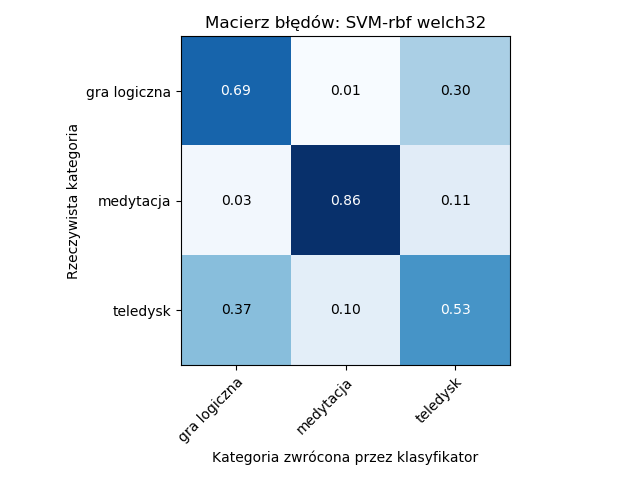
\includegraphics[width=1.3\linewidth]{rbf_svm_welch_32_cm.png}
	\end{minipage}
	\begin{minipage}{0.48\textwidth}
		\centering
		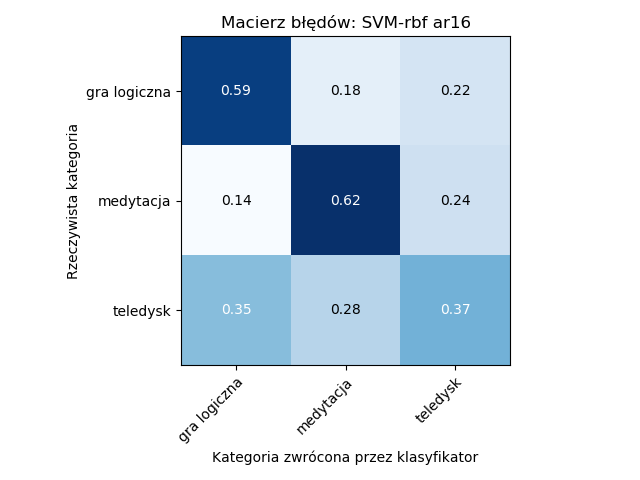
\includegraphics[width=1.3\linewidth]{rbf_svm_ar_16_cm.png}
	\end{minipage}
	\caption{Znormalizowana macierz błędów dla klasyfikatora SVM z radialną funkcją rdzenia i parametrów $C=10$, $\gamma=10$ oraz metody parametryzacji \textit{welch32} (lewa strona). Znormalizowana macierz błędów dla klasyfikatora SVM z radialną funkcją rdzenia i parametrów $C=1$, $\gamma=0.1$ oraz metody parametryzacji \textit{ar16}  (prawa strona).}
\end{figure}

\begin{figure}[H]
	\begin{minipage}{0.48\textwidth}
		\centering
		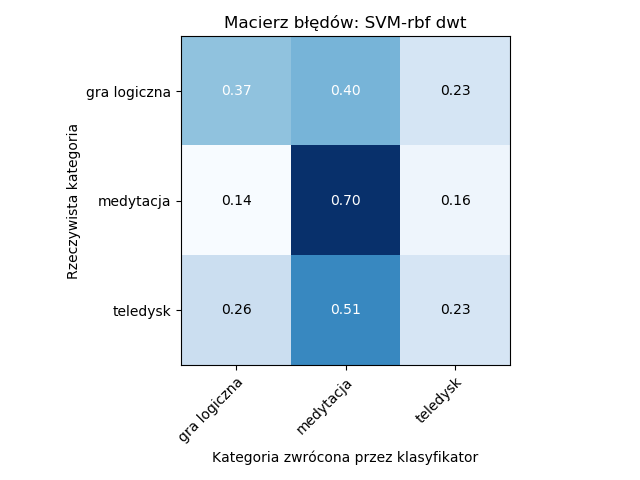
\includegraphics[width=1.3\linewidth]{rbf_svm_dwt_cm.png}
	\end{minipage}
	\begin{minipage}{0.48\textwidth}
		\centering
		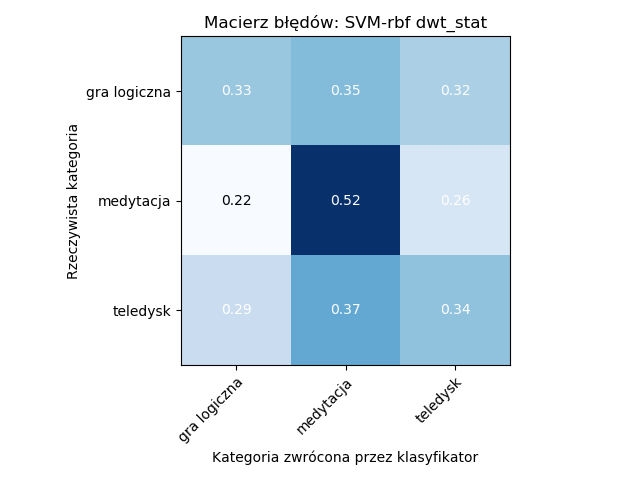
\includegraphics[width=1.3\linewidth]{rbf_svm_dwt_2_cm.png}
	\end{minipage}
	\caption{Znormalizowana macierz błędów dla klasyfikatora SVM z radialną funkcją rdzenia i parametrami $C=1$, $\gamma=1$ oraz metody parametryzacji \textit{dwt} (lewa strona). Znormalizowana macierz błędów dla klasyfikatora SVM z radialną funkcją rdzenia i parametrów $C=0.01$, $\gamma=0.1$ oraz metody parametryzacji \textit{dwt\_stat} (prawa strona).}
\end{figure}

Macierz błędów dla wariantu \textit{dwt} wygląda z kolei bardzo odmiennie od macierzy uzyskanych we wcześniejszych eksperymentach, w których większość ramek została zakwalifikowana do kategorii \textit{gra logiczna} lub \textit{teledysk} z prawie całkowitym pominięciem kategorii \textit{medytacja}. W obecnie omawianym eksperymencie większość ramek klasy \textit{medytacja} klasyfikowana jest poprawnie, natomiast ramki pozostałych klas są przyporządkowywane w różnych proporcjach do wszystkich kategorii, najczęściej jednak do klasy \textit{medytacja}. 

W przypadku wariantu \textit{dwt\_stat} ramki klas \textit{gra logiczna} oraz \textit{teledysk} są przyporządkowywane do trzech klas mniej więcej po równo. Ramki klasy \textit{medytacja} są w połowie przypadków brane za ramki pozostałych klas.

W tablicy 6.6 przedstawiono wartości precyzji, czułości oraz miary $F_1$ dla każdej z klas dla metod parametryzacji \textit{welch32}, \textit{ar16}, \textit{dwt} oraz \textit{dwt\_stat}. W wariantach \textit{welch32} oraz \textit{ar16} wartości wszystkich miar są najwyższe dla klasy \textit{medytacja}, a najniższe dla klasy \textit{teledysk}. W wariancie \textit{dwt} zwraca uwagę relatywnie niska precyzja dla klasy \textit{medytacja}.

\begin{table}[H]
	\centering
	\small
	\setlength\tabcolsep{2pt}
	\begin{tabular}{| c | c | c | c | c |}
		\hline
		Wariant & Klasa & Precyzja  & Czułość & Miara $F_1$ \\ \hline
		\multirow{3}{*}{} \textit{welch32} & \textit{medytacja} & 0.8876 & 0.8597 & 0.8735 \\
		C = 10 & \textit{gra logiczna} & 0.6287 & 0.6898 & 0.6578\\
		$\gamma$ = 10 & \textit{teledysk} & 0.5676 & 0.5302 & 0.5483\\ \hline
		\multirow{3}{*}{} \textit{ar16} & \textit{medytacja} & 0.5716 & 0.6203 & 0.5950 \\
		C = 1 & \textit{gra logiczna} & 0.5496 & 0.5931 & 0.5705\\
		$\gamma = 0.1$ & \textit{teledysk} & 0.4457 & 0.3724 & 0.4058\\ \hline
		\multirow{3}{*}{} \textit{dwt} & \textit{medytacja} & 0.4344 & 0.6983 & 0.5356 \\
		C = 1& \textit{gra logiczna} & 0.4791 & 0.3664 & 0.4152\\
		$\gamma$ = 1 & \textit{teledysk} & 0.3680 & 0.2310 & 0.2838\\ \hline
		\multirow{3}{*}{} \textit{dwt\_stat}& \textit{medytacja} & 0.4178 & 0.5193 & 0.4631 \\
		C = 0.01 & \textit{gra logiczna} & 0.3997 & 0.3337 & 0.3638\\
		$\gamma$ = 0.1 & \textit{teledysk} & 0.3685 & 0.3398 & 0.3536\\ \hline
	\end{tabular}
	\caption{Wartości precyzji, czułości oraz miary $F_1$ dla każdej z klas dla metod parametryzacji \textit{welch32}, \textit{ar16}, \textit{dwt} oraz \textit{dwt\_stat}.}
\end{table} 

\section{Eksperyment nr 4 - sieci neuronowe}
W ostatnim eksperymencie sprawdzono dokładność klasyfikacji ramek z użyciem sieci neuronowych. Do klasyfikacji użyto sieci neuronowych z pojedynczą warstwą ukrytą z funkcją aktywacji ReLU \cite{glorot} \cite{nair} oraz funkcją aktywacji \textit{softmax} w warstwie wyjściowej. Do inicjalizacji wag we wszystkich warstwach użyto metody He (parametr \textit{kernel\_initializer='he\_uniform'}) \cite{he}, natomiast składowe stałe zainicjalizowano zerami. Do uczenia modeli wykorzystano metodę gradientu stochastycznego z modyfikacją Nesterowa \cite{sutskever}. Parametr \textit{learning rate} ustawiono na wartość 0.01 ze spadkiem $10^{-6}$ na epokę. Współczynnik momentu ustawiono na wartość $\alpha=0.9$. Wykorzystano \textit{early stopping} z cierpliwością równą 50 epokom uczenia. Maksymalną możliwą liczbę epok uczenia ustawiono na 2000. Wyniki klasyfikacji przedstawiono w tablicy 6.7. Dalej przedstawiono kod użyty do uczenia sieci.

\begin{table}[H]
	\centering
	\small
	\setlength\tabcolsep{2pt}
	\begin{tabular}{| c | c | c | c | c | c | c |}
		\hline
		\multicolumn{7}{|c|}{Metoda parametryzacji} \\ \hline
		 \textit{ar16}  & \textit{ar24} & \textit{dwt} & \textit{dwt\_stat} & \textit{welch16} & \textit{welch32} & \textit{welch64} \\ \hline
		 0.5197 & 0.5330 & 0.3277 & 0.4992 & 0.6715 & \color{red} 0.7005 &  0.6868 \\ \hline	
	\end{tabular}
	\caption{Wyniki klasyfikacji ramek testowych za pomocą sieci neuronowych z jedną warstwą ukrytą.}
\end{table} 

W przeprowadzonym eksperymencie dla metod autoregresyjnych i falkowych  uzyskano podobne wyniki, jak dla SVM z liniową funkcją rdzenia, natomiast dla metody Welcha uzyskano jeszcze wyższe dokładności klasyfikacji niż w poprzednich eksperymentach. Ponownie najlepiej spisał się wariant \textit{welch32}, dla którego po raz pierwszy uzyskano dokładność klasyfikacji wyższą niż 70\%.
\newpage
\begin{lstlisting}
# uczenie sieci neuronowych z pojedynczą warstwą ukrytą
# oraz klasyfikacja danych testowych
from keras.layers import Dense, Activation
from keras.models import Sequential
from keras.optimizers import SGD
from keras.callbacks import EarlyStopping
n_inputs = reduced_train_data.shape[1]
model = Sequential()
model.add(Dense(n_inputs,activation='relu',input_dim=n_inputs,
	kernel_initializer='he_uniform',bias_initializer='zeros'))
model.add(Dense(3,activation='softmax',
	kernel_initializer='he_uniform',bias_initializer='zeros'))
sgd = SGD(lr=0.01,decay=1e-6,momentum=0.9,nesterov=True)
model.compile(loss='categorical_crossentropy',
	optimizer=sgd,metrics=['accuracy'])
es = EarlyStopping(monitor='val_loss',mode='min',
	patience=50,restore_best_weights=True)
history = model.fit(reduced_train_data,train_data_classes,batch_size=64,
	validation_data=(reduced_val_data,val_data_classes),
	callbacks=[es],epochs=2000)
predictions = model.predict(reduced_test_data,batch_size=128)
score = model.evaluate(reduced_test_data,
	test_data_classes,batch_size=128)
\end{lstlisting}

W związku z tym, że w każdym z przeprowadzonych eksperymentów wariant \textit{welch32} zapewniał najlepsze wyniki, w dalszej części eksperymentu postanowiono wykorzystać tylko tę metodę parametryzacji i skoncentrować się na strojeniu sieci neuronowej w celu uzyskania możliwie najlepszego wyniku. 

Specyfikację oraz sposób trenowania sieci neuronowych, dla których uzyskano najlepsze wyniki, przedstawiono w tablicy 6.8. Wszystkie opisane sieci mają warstwy wyjściowe złożone z 3 neuronów z funkcją aktywacji \textit{softmax}. Wagi wszystkich sieci zainicjalizowano metodą He, natomiast składowe stałe zainicjalizowano zerami. Do uczenia sieci wykorzystano metodę gradientu stochastycznego z momentem oraz modyfikacją Nesterowa. Najlepszy wynik zaznaczono kolorem czerwonym - jest to jednocześnie najlepszy wynik ze wszystkich wykonanych eksperymentów.
 \begin{table}[H]
	\centering
	\small
	\setlength\tabcolsep{2pt}
	\begin{tabular}{| c | c | c | c | c | c| }
		\hline
		\multirow{2}{*}{}
		Liczba warstw & funkcja & parametry & cierp- & maksymalna & dokładność \\
		ukrytych & aktywacji & SGD & liwość & liczba epok & klasyfikacji \\ \hline
		\multirow{3}{*}{} & & \textit{lr} = 0.01 & & & \\
		3 & \textit{LReLU} & \textit{decay} = $10^{-6}$ & 50 & 2000 & \color{red} 0.7477 \\ 
		& (\textit{a} = 0.2) & \textit{momentum} = 0.9 & & & \\ \hline 
		\multirow{3}{*}{} & \textit{tanh} +  & \textit{lr} = 0.005 & & & \\
		4 & \textit{LReLU} & \textit{decay} = $10^{-6}$ & 250 & 3000 & 0.7469 \\ 
		& (\textit{a} = 0.2) & \textit{momentum} = 0.9 & & & \\ \hline
		\multirow{3}{*}{} & & \textit{lr} = 0.01 & & & \\
		6 & \textit{ReLU} & \textit{decay} = $10^{-6}$ & 70 & 2000 & 0.7467 \\ 
		& & \textit{momentum} = 0.9 & & & \\ \hline 
		\multirow{3}{*}{} &  & \textit{lr} = 0.01 & & & \\
		3 & \textit{tanh} & \textit{decay} = $10^{-6}$ & 250 & 3000 & 0.7446 \\ 
		& & \textit{momentum} = 0.9 & & & \\ \hline
	\end{tabular}
	\caption{Konfiguracje sieci neuronowych dla których uzyskano najwyższe dokładności klasyfikacji.}
\end{table} 
Na rysunku 6.7 przedstawiono znormalizowaną macierz błędów dla najlepszej konfiguracji. Można zauważyć, że lepsze wyniki klasyfikacji w porównaniu do klasyfikatora SVM-RBF wynikają z wyższej czułości dla kategorii \textit{teledysk}. Czułości dla pozostałych klas pozostały na podobnym poziomie.

\begin{figure}[H]
	\centering
	\makebox[\textwidth][c]{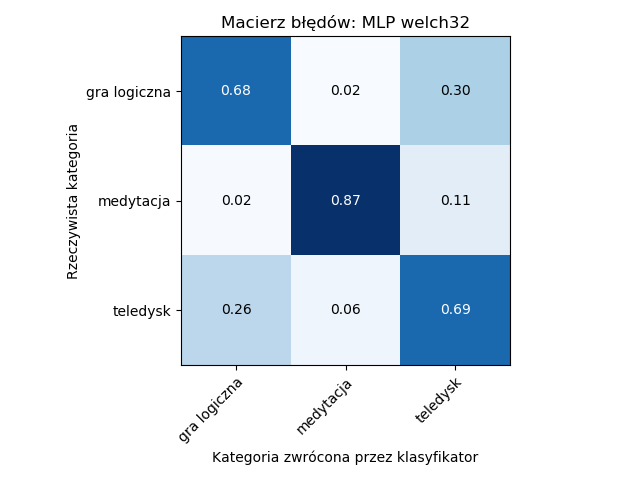
\includegraphics[width=0.9\textwidth]{mlp_i_7_welch_32_cm.png}}%
	\caption{Znormalizowana macierz błędów dla trójwarstwowej sieci neuronowej z funkcją aktywacji \textit{Leaky ReLU} i metody parametryzacji \textit{welch32}.}
\end{figure}

W tablicy 6.9 przedstawiono wartości precyzji, czułości oraz miary $F_1$ dla każdej z klas dla najlepszej konfiguracji sieci neuronowej. Tak samo jak w poprzednich eksperymentach wartości miar są najwyższe dla klasy \textit{medytacja}, a najniższe dla klasy \textit{teledysk}. Uwagę zwraca duży wzrost wartości miar, przede wszystkim czułości, dla klasy \textit{teledysk}, 13 punktów procentowych w porównaniu do SVM-RBF oraz 21 punktów procentowych w porównaniu do $k$-NN.

 \begin{table}[H]
	\centering
	\small
	\setlength\tabcolsep{2pt}
	\begin{tabular}{| c | c | c | c |}
		\hline
	 Klasa & Precyzja  & Czułość & Miara $F_1$ \\ \hline
	 \textit{medytacja} & 0.9203 & 0.8724 & 0.8957 \\
	 \textit{gra logiczna} & 0.7116 & 0.6832 & 0.6971\\
	 \textit{teledysk} & 0.6296 & 0.6874 & 0.6572\\ \hline
	\end{tabular}
	\caption{Wartości precyzji, czułości oraz miary $F_1$ dla każdej z klas  dla trójwarstwowej sieci neuronowej z funkcją aktywacji \textit{Leaky ReLU} i metody parametryzacji \textit{welch32}.}
\end{table}

Zastosowanie niżej przedstawionych technik nie spowodowało polepszenia dokładności klasyfikacji, a nawet ją pogorszyło:
\begin{itemize}
	\item dodawanie kolejnych warstw ukrytych,
	\item stosowanie funkcji aktywacji \textit{PReLU},
	\item stosowanie adaptacyjnych metod optymalizacji
	\item stosowanie warstw \textit{batch normalization} oraz \textit{dropout},
	\item stosowanie regularyzacji $L^1$ i $L^2$,
	\item uzupełnienie wektora cech o skośność, kurtozę oraz energię sygnału obliczonych w każdym kanale dla surowych (nieprzetworzonych) ramek.
\end{itemize}

Na rysunkach 6.8 i 6.9 wykreślono dwie pierwsze składowe główne zbiorów danych treningowych i testowych sparametryzowanych metodą \textit{welch32}. Dwie pierwsze składowe główne w tym przypadku odpowiadają za odpowiednio 12.87\% i 4.33\% wariancji zbioru treningowego. Jak widać, możliwe jest poprowadzenie granicy decyzyjnej w taki sposób, aby większość obserwacji należących do klas \textit{medytacja} oraz \textit{gra logiczna} zostało poprawnie zaklasyfikowanych. Obserwacje klasy \textit{teledysk} są problematyczne, gdyż mieszają się z obserwacjami pozostałych klas - w szczególności z obserwacjami klasy \textit{gra logiczna}. W celu dalszego poprawienia dokładności klasyfikacji kluczową kwestią jest więc znalezienie cech, które umożliwią odseparowanie obserwacji klasy \textit{teledysk} od obserwacji dwóch pozostałych klas.

\begin{figure}[H]
	\centering
	\makebox[\textwidth][c]{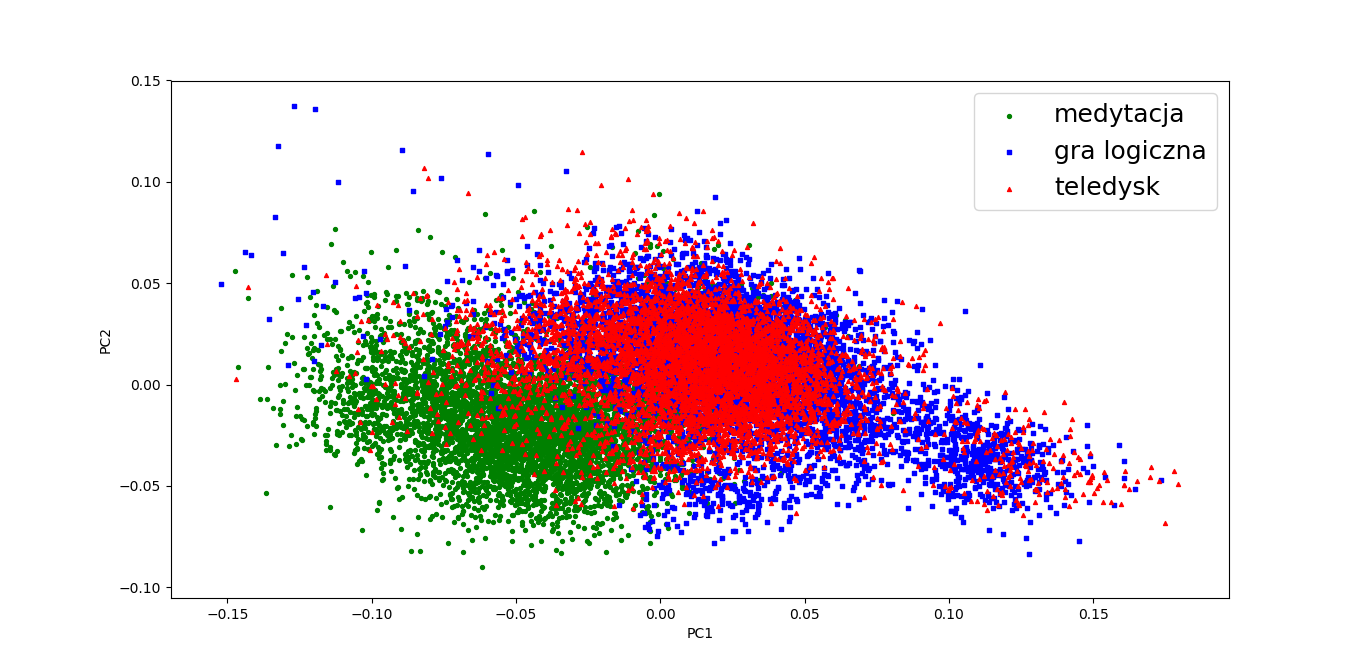
\includegraphics[width=1.3\textwidth]{pca_train_big_2.png}}%
	\caption{Pierwsza (oś odciętych) i druga (oś rzędnych) składowa główna zbioru danych treningowych sparametryzowanych metodą \textit{welch32}.}
\end{figure}

\begin{figure}[H]
	\centering
	\makebox[\textwidth][c]{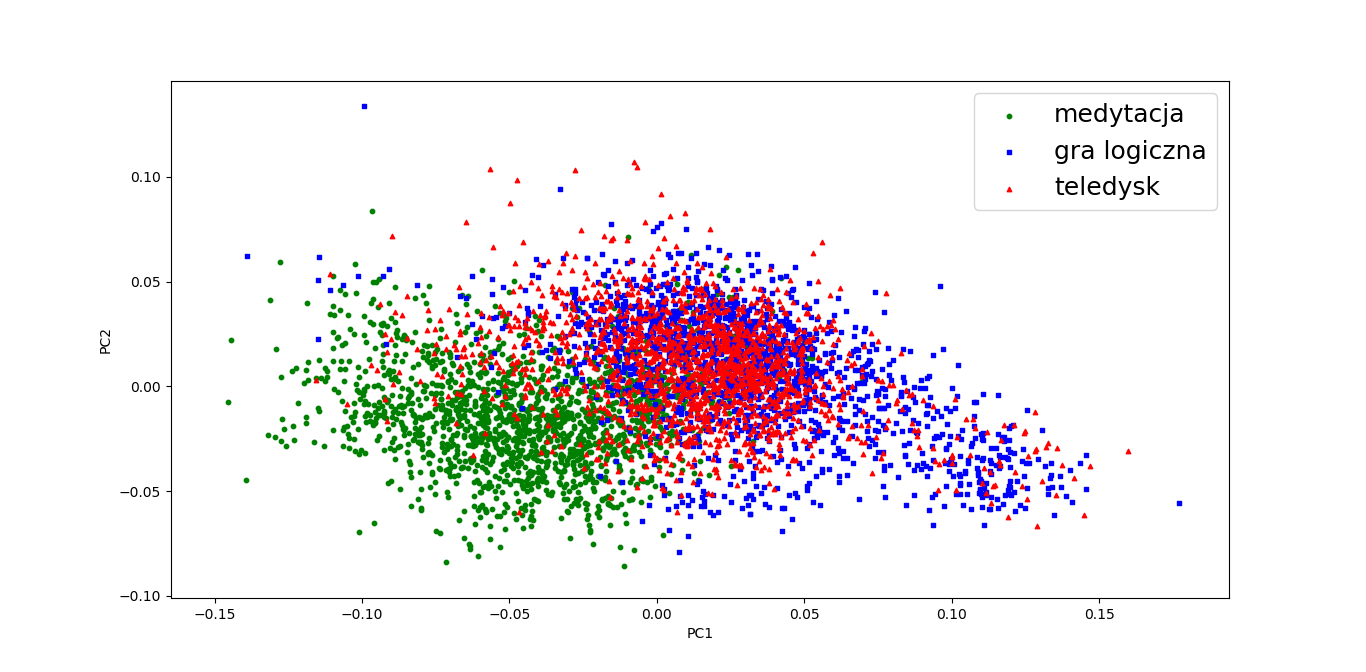
\includegraphics[width=1.3\textwidth]{pca_test_big_3.png}}%
	\caption{Pierwsza (oś odciętych) i druga (oś rzędnych) składowa główna zbioru danych testowych sparametryzowanych metodą \textit{welch32}.}
\end{figure}

\chapter*{Podsumowanie}
\addcontentsline{toc}{chapter}{Podsumowanie} \markboth{Podsumowanie}{}
Celem pracy było porównanie skuteczności wybranych metod analizy sygnałów oraz metod klasyfikacji w zadaniu rozpoznawania trzech stanów mentalnych - \textit{medytacja}, \textit{gra logiczna} oraz \textit{teledysk} - na bazie zarejestrowanego sygnału EEG. Dane zostały wstępnie przetworzone poprzez analizę składowych niezależnych. Do parametryzacji sygnału użyto modelowania autoregresyjnego, metody Welcha oraz dyskretnej transformacji falkowej. Wektory cech zostały zredukowane za pomocą analizy składowych głównych. Klasyfikacji dokonano za pomocą metody $k$-najbliższych sąsiadów, maszyn wektorów nośnych oraz sieci neuronowych. 

Spośród testowanych metod analizy sygnału najlepsze wyniki zostały osiągnięte dla metody Welcha, zaś najbardziej skutecznym klasyfikatorem okazała się sieć neuronowa. Wybór metody parametryzacji okazał się mieć dużo większy wpływ na ostateczną dokładność klasyfikacji, niż wybór klasyfikatora. 

Głównym czynnikiem ograniczającym dokładność klasyfikacji była trudność oddzielenia obserwacji klasy \textit{teledysk} od obserwacji pozostałych klas. Sugeruje to konieczność opracowania zestawu cech umożliwiającego lepszą separację klas. Istnieje też możliwość wprowadzenia dodatkowej fazy medytacji pomiędzy fazę \textit{teledysk} oraz \textit{gra logiczna}. Prawdopodobnie pozwoliłoby to na uzyskanie lepszej separacji sygnałowej tych dwóch aktywnych faz, a co za tym idzie – większej skuteczności klasyfikacji.

Ze względu na ograniczoną objętość pracy oraz ograniczony czas nie zostały przetestowane niektóre możliwe warianty użytych metod. W przeprowadzonych eksperymentach użyto współczynników modelu autoregresyjnego w roli cech. Innym możliwym podejściem jest obliczenie estymaty widmowej gęstości mocy na podstawie uzyskanego modelu autoregresyjnego. Pozostałe czynniki których wpływu nie zbadano to: wpływ algorytmu ICA na wyniki klasyfikacji, wpływ wstępnego usuwania składowej stałej oraz wybielania ramek danych, wpływ długości ramki danych (również w kontekście kompromisu między długością ramki a liczbą obserwacji treningowych), wpływ długości zakładki, a także w przypadku dyskretnej transformacji falkowej - wpływ użytej falki. Przetestowanie wpływu tych czynników może stanowić dalszy kierunek prowadzenia badań w tym temacie.

Innym możliwym kierunkiem dalszego prowadzenia badań byłoby zastosowanie dwuwymiarowych metod parametryzacji (np. dwuwymiarowej transformacji falkowej), uwzględniających położenie danej elektrody. Do klasyfikacji otrzymanych w ten sposób macierzy danych można wykorzystać splotowe sieci neuronowe (ang. \textit{Convolutional Neural Network, CNN}). Splotowe sieci neuronowe zostały już z powodzeniem zastosowane do detekcji wstrząsów epileptycznych na podstawie sygnału EEG \cite{acharya}.

%\nocite{*}
\cleardoublepage
\phantomsection
\addcontentsline{toc}{chapter}{Bibliografia}
\printbibliography

%\cleardoublepage
%\phantomsection
%\addcontentsline{toc}{chapter}{\listfigurename}
\listoffigures%\newpage
%\cleardoublepage
%\phantomsection
%\addcontentsline{toc}{chapter}{\listtablename}
\listoftables%\newpage

\end{document}